\documentclass{beamer}\usepackage[]{graphicx}\usepackage[]{color}
%% maxwidth is the original width if it is less than linewidth
%% otherwise use linewidth (to make sure the graphics do not exceed the margin)
\makeatletter
\def\maxwidth{ %
  \ifdim\Gin@nat@width>\linewidth
    \linewidth
  \else
    \Gin@nat@width
  \fi
}
\makeatother

\definecolor{fgcolor}{rgb}{1, 0.894, 0.769}
\newcommand{\hlnum}[1]{\textcolor[rgb]{0.824,0.412,0.118}{#1}}%
\newcommand{\hlstr}[1]{\textcolor[rgb]{1,0.894,0.71}{#1}}%
\newcommand{\hlcom}[1]{\textcolor[rgb]{0.824,0.706,0.549}{#1}}%
\newcommand{\hlopt}[1]{\textcolor[rgb]{1,0.894,0.769}{#1}}%
\newcommand{\hlstd}[1]{\textcolor[rgb]{1,0.894,0.769}{#1}}%
\newcommand{\hlkwa}[1]{\textcolor[rgb]{0.941,0.902,0.549}{#1}}%
\newcommand{\hlkwb}[1]{\textcolor[rgb]{0.804,0.776,0.451}{#1}}%
\newcommand{\hlkwc}[1]{\textcolor[rgb]{0.78,0.941,0.545}{#1}}%
\newcommand{\hlkwd}[1]{\textcolor[rgb]{1,0.78,0.769}{#1}}%
\let\hlipl\hlkwb

\usepackage{framed}
\makeatletter
\newenvironment{kframe}{%
 \def\at@end@of@kframe{}%
 \ifinner\ifhmode%
  \def\at@end@of@kframe{\end{minipage}}%
  \begin{minipage}{\columnwidth}%
 \fi\fi%
 \def\FrameCommand##1{\hskip\@totalleftmargin \hskip-\fboxsep
 \colorbox{shadecolor}{##1}\hskip-\fboxsep
     % There is no \\@totalrightmargin, so:
     \hskip-\linewidth \hskip-\@totalleftmargin \hskip\columnwidth}%
 \MakeFramed {\advance\hsize-\width
   \@totalleftmargin\z@ \linewidth\hsize
   \@setminipage}}%
 {\par\unskip\endMakeFramed%
 \at@end@of@kframe}
\makeatother

\definecolor{shadecolor}{rgb}{.97, .97, .97}
\definecolor{messagecolor}{rgb}{0, 0, 0}
\definecolor{warningcolor}{rgb}{1, 0, 1}
\definecolor{errorcolor}{rgb}{1, 0, 0}
\newenvironment{knitrout}{}{} % an empty environment to be redefined in TeX

\usepackage{alltt}
\usepackage{../371g-slides}
\title{Time Series: Smoothing \& Moving Average}
\subtitle{Lecture 19}
\author{STA 371G}
\IfFileExists{upquote.sty}{\usepackage{upquote}}{}
\begin{document}
  
  

  \frame{\maketitle}

  % Show outline at beginning of each section 
  \AtBeginSection[]{ 
    \begin{frame}<beamer>
      \tableofcontents[currentsection]
    \end{frame}
  }

  %%%%%%% Slides start here %%%%%%%

  \begin{darkframes}
    
    \begin{frame}{Trend \& Seasonality in Time Series}
      \fontsize{9}{9 }\selectfont
      \begin{center}
        \includegraphics[width=2.8in]{nashville} \\
      \end{center} 
      
      \begin{itemize}[<+->]
        \item Although desired, most of the time series data are not stationary.
        \item Two main factors that make data non-stationary: Trend and seasonality.
        \item Sales, economic, activity etc. data often show strong seasonality.
        \item E.g. Quarterly totals of international airline passengers, 1949 to 1960.
      \end{itemize}
      
    \end{frame}
    
    
 
    
    
    
    \begin{frame}[fragile]{Airline Passengers 1949-1960}
      \fontsize{8}{8}\selectfont
\begin{knitrout}
\definecolor{shadecolor}{rgb}{0.137, 0.137, 0.137}\begin{kframe}
\begin{alltt}
\hlcom{# Convert data into time series, starting from 1st quarter of 1949.}
\hlstd{air} \hlkwb{<-} \hlkwd{ts}\hlstd{(air_passengers}\hlopt{$}\hlstd{number,} \hlkwc{start}\hlstd{=}\hlkwd{c}\hlstd{(}\hlnum{1949}\hlstd{,}\hlnum{1}\hlstd{),} \hlkwc{frequency}\hlstd{=}\hlnum{4}\hlstd{)}
\hlcom{# Frequency: 4 data points per year (this is quarterly data)}
\hlkwd{plot}\hlstd{(air,} \hlkwc{ylab}\hlstd{=}\hlstr{"# of International Passengers ('000)"}\hlstd{)}
\end{alltt}
\end{kframe}
\input{/tmp/figures/unnamed-chunk-2-1.tikz}

\end{knitrout}
    \end{frame}
    
    
    \begin{frame}{What is seasonality, exactly?}
      \fontsize{9}{9}\selectfont
      
      \begin{itemize}[<+->]
        \item Seasonality: The presence of variations that occur at specific regular intervals in a season.
        \item In this case, a season is a year.
        \item The frequency, the number of observations in a season, is 4. 
        \item The data behaves similarly in the same quarter of different years.
        \item E.g. every year, the number of passengers peaks in the 3rd quarter. Similarly, it dips in the 4th quarter.
      \end{itemize}
      
    \end{frame}
    
    
    \begin{frame}[fragile]{Exploring the data}
      \fontsize{9}{9}\selectfont
        \begin{itemize}[<+->]
        \item Overall, there is an upward trend in the number of airline passengers between 1949-1960.
        
        \item The seasonality in the data makes it difficult to see how the trend changes over years.
        
        \item E.g. it is not clear wether the number is increasing at the same rate every year, or the rate varies in different years. 
        
        \item The trend in the data makes it difficult to see the impact of seasonality in the data. 
        
        \item E.g. it is not clear why the 2nd quarters are higher than the 1st quarters: Is it a more active traveling period of the year or is it just more people are using air travel as time goes by?
        
        \item Smoothing the data helps identifying the trend and seasonal effects in a clearer way.
        
        \lc
      \end{itemize}
    \end{frame}
    
    
    
    \begin{frame}[fragile]{Smoothing the data: one-sided moving average}
    \fontsize{9}{9}\selectfont
        
        \alert{(One-sided) Moving average} is a simple average of all observations over the previous season (year).
        
        \begin{center}
          $y_t:$ Number of passengers traveled at time $t$
        \end{center}  
        
        One-sided moving average at time $t$:
        
        \begin{center}
          $m_t = \frac{1}{4} y_{t-3} + \frac{1}{4} y_{t-2} + \frac{1}{4} y_{t-1} + \frac{1}{4} y_{t}$
        \end{center}  
        Each quarter has equal weight in the moving average.
        
    \end{frame}
    
    
    
    \begin{frame}[fragile]{Smoothing the data: one-sided moving average}
      \fontsize{9}{9}\selectfont
      \begin{center}
          \begin{tabular}{llllllll}
          \hline
            & Y49Q1 & Y49Q2 & Y49Q3 & Y49Q4 & Y50Q1 & Y50Q2 & ... \\
          \hline
           $t$ & 1  &	2 &	3 &	4 &	5 &	6 & ... \\
          $y_t$ & 362 &	385 &	432 &	341 &	382 &	409 & ... \\
          $m_t$ & NA &	NA &	NA &	380	& 385	& 391 & ... \\
            \hline 
        \end{tabular}
      \end{center} \pause
      
      \begin{center}
        \begin{eqnarray*}
          m_4 &=& \frac{1}{4} y_{1} + \frac{1}{4} y_{2} + \frac{1}{4} y_{3} + \frac{1}{4} y_{4} \\
          &=& \frac{1}{4} 362 + \frac{1}{4} 385 + \frac{1}{4} 432 + \frac{1}{4} 341 \\
          &=& 380
        \end{eqnarray*}
      \end{center} 
      
    \end{frame}
    
    
    

    \begin{frame}[fragile]{Smoothing the data: one-sided moving average}
      \fontsize{8}{8}\selectfont
  
\begin{knitrout}
\definecolor{shadecolor}{rgb}{0.137, 0.137, 0.137}\begin{kframe}
\begin{alltt}
\hlcom{# One sided moving average}
\hlstd{air_ma_one} \hlkwb{<-} \hlkwd{filter}\hlstd{(air,} \hlkwc{filter}\hlstd{=}\hlkwd{c}\hlstd{(}\hlnum{1}\hlopt{/}\hlnum{4}\hlstd{,}\hlnum{1}\hlopt{/}\hlnum{4}\hlstd{,}\hlnum{1}\hlopt{/}\hlnum{4}\hlstd{,}\hlnum{1}\hlopt{/}\hlnum{4}\hlstd{),} \hlkwc{sides}\hlstd{=}\hlnum{1}\hlstd{)}
\hlkwd{plot}\hlstd{(air,} \hlkwc{ylab}\hlstd{=}\hlstr{"# of International Passengers ('000)"}\hlstd{)}
\hlkwd{lines}\hlstd{(air_ma_one,} \hlkwc{col}\hlstd{=}\hlstr{'green'}\hlstd{)}
\end{alltt}
\end{kframe}
\input{/tmp/figures/unnamed-chunk-3-1.tikz}

\end{knitrout}
    
    \end{frame}
    
    
    
    
    \begin{frame}[fragile]{Smoothing the data}
      \fontsize{9}{9}\selectfont
      Smoothed data better shows the slow-downs in the trend around 1954 and 1959.
      \bigskip
      
      Let's also see the effect of the seasonality by eliminating the trend in the data. This is called \alert{detrending}.

    \end{frame}
    
    
    
    \begin{frame}[fragile]{Smoothing the data}
      \fontsize{9}{9}\selectfont
      When trend and seasonality are additive
      \begin{center}
        Data = Trend + Seasonality + Randomness
      \end{center}
     
\begin{knitrout}
\definecolor{shadecolor}{rgb}{0.137, 0.137, 0.137}\begin{kframe}
\begin{alltt}
      \hlstd{air_seasonal_additive} \hlkwb{<-} \hlstd{air} \hlopt{-} \hlstd{air_ma_one}
      \hlkwd{plot}\hlstd{(air_seasonal_additive)}
\end{alltt}
\end{kframe}
\input{/tmp/figures/unnamed-chunk-4-1.tikz}

\end{knitrout}
  
    \end{frame}
    
    
      \begin{frame}[fragile]{Smoothing the data}
      \fontsize{9}{9}\selectfont
        When trend and seasonality are multiplicative
      \begin{center}
        Data = Trend $\times$ Seasonality $\times$ Randomness
      \end{center}
     
\begin{knitrout}
\definecolor{shadecolor}{rgb}{0.137, 0.137, 0.137}\begin{kframe}
\begin{alltt}
      \hlstd{air_seasonal_multiplicative} \hlkwb{<-} \hlstd{air}\hlopt{/} \hlstd{air_ma_one}
      \hlkwd{plot}\hlstd{(air_seasonal_multiplicative)}
\end{alltt}
\end{kframe}
% Created by tikzDevice version 0.10.1 on 2017-03-08 23:30:47
% !TEX encoding = UTF-8 Unicode
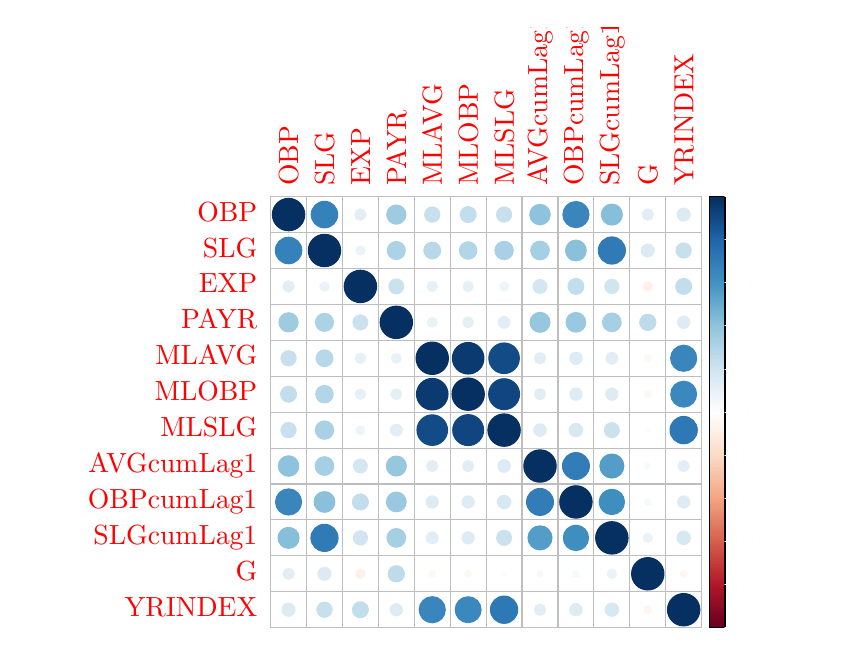
\begin{tikzpicture}[x=1pt,y=1pt]
\definecolor{fillColor}{RGB}{255,255,255}
\path[use as bounding box,fill=fillColor,fill opacity=0.00] (0,0) rectangle (289.08,216.81);
\begin{scope}
\path[clip] (  0.00,  0.00) rectangle (289.08,216.81);
\definecolor{drawColor}{RGB}{255,255,255}
\definecolor{fillColor}{RGB}{255,255,255}

\path[draw=drawColor,line width= 0.4pt,line join=round,line cap=round,fill=fillColor] ( 87.78,142.78) rectangle (100.76,155.76);

\path[draw=drawColor,line width= 0.4pt,line join=round,line cap=round,fill=fillColor] ( 87.78,129.80) rectangle (100.76,142.78);

\path[draw=drawColor,line width= 0.4pt,line join=round,line cap=round,fill=fillColor] ( 87.78,116.82) rectangle (100.76,129.80);

\path[draw=drawColor,line width= 0.4pt,line join=round,line cap=round,fill=fillColor] ( 87.78,103.84) rectangle (100.76,116.82);

\path[draw=drawColor,line width= 0.4pt,line join=round,line cap=round,fill=fillColor] ( 87.78, 90.86) rectangle (100.76,103.84);

\path[draw=drawColor,line width= 0.4pt,line join=round,line cap=round,fill=fillColor] ( 87.78, 77.88) rectangle (100.76, 90.86);

\path[draw=drawColor,line width= 0.4pt,line join=round,line cap=round,fill=fillColor] ( 87.78, 64.90) rectangle (100.76, 77.88);

\path[draw=drawColor,line width= 0.4pt,line join=round,line cap=round,fill=fillColor] ( 87.78, 51.92) rectangle (100.76, 64.90);

\path[draw=drawColor,line width= 0.4pt,line join=round,line cap=round,fill=fillColor] ( 87.78, 38.94) rectangle (100.76, 51.92);

\path[draw=drawColor,line width= 0.4pt,line join=round,line cap=round,fill=fillColor] ( 87.78, 25.96) rectangle (100.76, 38.94);

\path[draw=drawColor,line width= 0.4pt,line join=round,line cap=round,fill=fillColor] ( 87.78, 12.98) rectangle (100.76, 25.96);

\path[draw=drawColor,line width= 0.4pt,line join=round,line cap=round,fill=fillColor] ( 87.78,  0.00) rectangle (100.76, 12.98);

\path[draw=drawColor,line width= 0.4pt,line join=round,line cap=round,fill=fillColor] (100.76,142.78) rectangle (113.74,155.76);

\path[draw=drawColor,line width= 0.4pt,line join=round,line cap=round,fill=fillColor] (100.76,129.80) rectangle (113.74,142.78);

\path[draw=drawColor,line width= 0.4pt,line join=round,line cap=round,fill=fillColor] (100.76,116.82) rectangle (113.74,129.80);

\path[draw=drawColor,line width= 0.4pt,line join=round,line cap=round,fill=fillColor] (100.76,103.84) rectangle (113.74,116.82);

\path[draw=drawColor,line width= 0.4pt,line join=round,line cap=round,fill=fillColor] (100.76, 90.86) rectangle (113.74,103.84);

\path[draw=drawColor,line width= 0.4pt,line join=round,line cap=round,fill=fillColor] (100.76, 77.88) rectangle (113.74, 90.86);

\path[draw=drawColor,line width= 0.4pt,line join=round,line cap=round,fill=fillColor] (100.76, 64.90) rectangle (113.74, 77.88);

\path[draw=drawColor,line width= 0.4pt,line join=round,line cap=round,fill=fillColor] (100.76, 51.92) rectangle (113.74, 64.90);

\path[draw=drawColor,line width= 0.4pt,line join=round,line cap=round,fill=fillColor] (100.76, 38.94) rectangle (113.74, 51.92);

\path[draw=drawColor,line width= 0.4pt,line join=round,line cap=round,fill=fillColor] (100.76, 25.96) rectangle (113.74, 38.94);

\path[draw=drawColor,line width= 0.4pt,line join=round,line cap=round,fill=fillColor] (100.76, 12.98) rectangle (113.74, 25.96);

\path[draw=drawColor,line width= 0.4pt,line join=round,line cap=round,fill=fillColor] (100.76,  0.00) rectangle (113.74, 12.98);

\path[draw=drawColor,line width= 0.4pt,line join=round,line cap=round,fill=fillColor] (113.74,142.78) rectangle (126.72,155.76);

\path[draw=drawColor,line width= 0.4pt,line join=round,line cap=round,fill=fillColor] (113.74,129.80) rectangle (126.72,142.78);

\path[draw=drawColor,line width= 0.4pt,line join=round,line cap=round,fill=fillColor] (113.74,116.82) rectangle (126.72,129.80);

\path[draw=drawColor,line width= 0.4pt,line join=round,line cap=round,fill=fillColor] (113.74,103.84) rectangle (126.72,116.82);

\path[draw=drawColor,line width= 0.4pt,line join=round,line cap=round,fill=fillColor] (113.74, 90.86) rectangle (126.72,103.84);

\path[draw=drawColor,line width= 0.4pt,line join=round,line cap=round,fill=fillColor] (113.74, 77.88) rectangle (126.72, 90.86);

\path[draw=drawColor,line width= 0.4pt,line join=round,line cap=round,fill=fillColor] (113.74, 64.90) rectangle (126.72, 77.88);

\path[draw=drawColor,line width= 0.4pt,line join=round,line cap=round,fill=fillColor] (113.74, 51.92) rectangle (126.72, 64.90);

\path[draw=drawColor,line width= 0.4pt,line join=round,line cap=round,fill=fillColor] (113.74, 38.94) rectangle (126.72, 51.92);

\path[draw=drawColor,line width= 0.4pt,line join=round,line cap=round,fill=fillColor] (113.74, 25.96) rectangle (126.72, 38.94);

\path[draw=drawColor,line width= 0.4pt,line join=round,line cap=round,fill=fillColor] (113.74, 12.98) rectangle (126.72, 25.96);

\path[draw=drawColor,line width= 0.4pt,line join=round,line cap=round,fill=fillColor] (113.74,  0.00) rectangle (126.72, 12.98);

\path[draw=drawColor,line width= 0.4pt,line join=round,line cap=round,fill=fillColor] (126.72,142.78) rectangle (139.70,155.76);

\path[draw=drawColor,line width= 0.4pt,line join=round,line cap=round,fill=fillColor] (126.72,129.80) rectangle (139.70,142.78);

\path[draw=drawColor,line width= 0.4pt,line join=round,line cap=round,fill=fillColor] (126.72,116.82) rectangle (139.70,129.80);

\path[draw=drawColor,line width= 0.4pt,line join=round,line cap=round,fill=fillColor] (126.72,103.84) rectangle (139.70,116.82);

\path[draw=drawColor,line width= 0.4pt,line join=round,line cap=round,fill=fillColor] (126.72, 90.86) rectangle (139.70,103.84);

\path[draw=drawColor,line width= 0.4pt,line join=round,line cap=round,fill=fillColor] (126.72, 77.88) rectangle (139.70, 90.86);

\path[draw=drawColor,line width= 0.4pt,line join=round,line cap=round,fill=fillColor] (126.72, 64.90) rectangle (139.70, 77.88);

\path[draw=drawColor,line width= 0.4pt,line join=round,line cap=round,fill=fillColor] (126.72, 51.92) rectangle (139.70, 64.90);

\path[draw=drawColor,line width= 0.4pt,line join=round,line cap=round,fill=fillColor] (126.72, 38.94) rectangle (139.70, 51.92);

\path[draw=drawColor,line width= 0.4pt,line join=round,line cap=round,fill=fillColor] (126.72, 25.96) rectangle (139.70, 38.94);

\path[draw=drawColor,line width= 0.4pt,line join=round,line cap=round,fill=fillColor] (126.72, 12.98) rectangle (139.70, 25.96);

\path[draw=drawColor,line width= 0.4pt,line join=round,line cap=round,fill=fillColor] (126.72,  0.00) rectangle (139.70, 12.98);

\path[draw=drawColor,line width= 0.4pt,line join=round,line cap=round,fill=fillColor] (139.70,142.78) rectangle (152.68,155.76);

\path[draw=drawColor,line width= 0.4pt,line join=round,line cap=round,fill=fillColor] (139.70,129.80) rectangle (152.68,142.78);

\path[draw=drawColor,line width= 0.4pt,line join=round,line cap=round,fill=fillColor] (139.70,116.82) rectangle (152.68,129.80);

\path[draw=drawColor,line width= 0.4pt,line join=round,line cap=round,fill=fillColor] (139.70,103.84) rectangle (152.68,116.82);

\path[draw=drawColor,line width= 0.4pt,line join=round,line cap=round,fill=fillColor] (139.70, 90.86) rectangle (152.68,103.84);

\path[draw=drawColor,line width= 0.4pt,line join=round,line cap=round,fill=fillColor] (139.70, 77.88) rectangle (152.68, 90.86);

\path[draw=drawColor,line width= 0.4pt,line join=round,line cap=round,fill=fillColor] (139.70, 64.90) rectangle (152.68, 77.88);

\path[draw=drawColor,line width= 0.4pt,line join=round,line cap=round,fill=fillColor] (139.70, 51.92) rectangle (152.68, 64.90);

\path[draw=drawColor,line width= 0.4pt,line join=round,line cap=round,fill=fillColor] (139.70, 38.94) rectangle (152.68, 51.92);

\path[draw=drawColor,line width= 0.4pt,line join=round,line cap=round,fill=fillColor] (139.70, 25.96) rectangle (152.68, 38.94);

\path[draw=drawColor,line width= 0.4pt,line join=round,line cap=round,fill=fillColor] (139.70, 12.98) rectangle (152.68, 25.96);

\path[draw=drawColor,line width= 0.4pt,line join=round,line cap=round,fill=fillColor] (139.70,  0.00) rectangle (152.68, 12.98);

\path[draw=drawColor,line width= 0.4pt,line join=round,line cap=round,fill=fillColor] (152.68,142.78) rectangle (165.66,155.76);

\path[draw=drawColor,line width= 0.4pt,line join=round,line cap=round,fill=fillColor] (152.68,129.80) rectangle (165.66,142.78);

\path[draw=drawColor,line width= 0.4pt,line join=round,line cap=round,fill=fillColor] (152.68,116.82) rectangle (165.66,129.80);

\path[draw=drawColor,line width= 0.4pt,line join=round,line cap=round,fill=fillColor] (152.68,103.84) rectangle (165.66,116.82);

\path[draw=drawColor,line width= 0.4pt,line join=round,line cap=round,fill=fillColor] (152.68, 90.86) rectangle (165.66,103.84);

\path[draw=drawColor,line width= 0.4pt,line join=round,line cap=round,fill=fillColor] (152.68, 77.88) rectangle (165.66, 90.86);

\path[draw=drawColor,line width= 0.4pt,line join=round,line cap=round,fill=fillColor] (152.68, 64.90) rectangle (165.66, 77.88);

\path[draw=drawColor,line width= 0.4pt,line join=round,line cap=round,fill=fillColor] (152.68, 51.92) rectangle (165.66, 64.90);

\path[draw=drawColor,line width= 0.4pt,line join=round,line cap=round,fill=fillColor] (152.68, 38.94) rectangle (165.66, 51.92);

\path[draw=drawColor,line width= 0.4pt,line join=round,line cap=round,fill=fillColor] (152.68, 25.96) rectangle (165.66, 38.94);

\path[draw=drawColor,line width= 0.4pt,line join=round,line cap=round,fill=fillColor] (152.68, 12.98) rectangle (165.66, 25.96);

\path[draw=drawColor,line width= 0.4pt,line join=round,line cap=round,fill=fillColor] (152.68,  0.00) rectangle (165.66, 12.98);

\path[draw=drawColor,line width= 0.4pt,line join=round,line cap=round,fill=fillColor] (165.66,142.78) rectangle (178.64,155.76);

\path[draw=drawColor,line width= 0.4pt,line join=round,line cap=round,fill=fillColor] (165.66,129.80) rectangle (178.64,142.78);

\path[draw=drawColor,line width= 0.4pt,line join=round,line cap=round,fill=fillColor] (165.66,116.82) rectangle (178.64,129.80);

\path[draw=drawColor,line width= 0.4pt,line join=round,line cap=round,fill=fillColor] (165.66,103.84) rectangle (178.64,116.82);

\path[draw=drawColor,line width= 0.4pt,line join=round,line cap=round,fill=fillColor] (165.66, 90.86) rectangle (178.64,103.84);

\path[draw=drawColor,line width= 0.4pt,line join=round,line cap=round,fill=fillColor] (165.66, 77.88) rectangle (178.64, 90.86);

\path[draw=drawColor,line width= 0.4pt,line join=round,line cap=round,fill=fillColor] (165.66, 64.90) rectangle (178.64, 77.88);

\path[draw=drawColor,line width= 0.4pt,line join=round,line cap=round,fill=fillColor] (165.66, 51.92) rectangle (178.64, 64.90);

\path[draw=drawColor,line width= 0.4pt,line join=round,line cap=round,fill=fillColor] (165.66, 38.94) rectangle (178.64, 51.92);

\path[draw=drawColor,line width= 0.4pt,line join=round,line cap=round,fill=fillColor] (165.66, 25.96) rectangle (178.64, 38.94);

\path[draw=drawColor,line width= 0.4pt,line join=round,line cap=round,fill=fillColor] (165.66, 12.98) rectangle (178.64, 25.96);

\path[draw=drawColor,line width= 0.4pt,line join=round,line cap=round,fill=fillColor] (165.66,  0.00) rectangle (178.64, 12.98);

\path[draw=drawColor,line width= 0.4pt,line join=round,line cap=round,fill=fillColor] (178.64,142.78) rectangle (191.62,155.76);

\path[draw=drawColor,line width= 0.4pt,line join=round,line cap=round,fill=fillColor] (178.64,129.80) rectangle (191.62,142.78);

\path[draw=drawColor,line width= 0.4pt,line join=round,line cap=round,fill=fillColor] (178.64,116.82) rectangle (191.62,129.80);

\path[draw=drawColor,line width= 0.4pt,line join=round,line cap=round,fill=fillColor] (178.64,103.84) rectangle (191.62,116.82);

\path[draw=drawColor,line width= 0.4pt,line join=round,line cap=round,fill=fillColor] (178.64, 90.86) rectangle (191.62,103.84);

\path[draw=drawColor,line width= 0.4pt,line join=round,line cap=round,fill=fillColor] (178.64, 77.88) rectangle (191.62, 90.86);

\path[draw=drawColor,line width= 0.4pt,line join=round,line cap=round,fill=fillColor] (178.64, 64.90) rectangle (191.62, 77.88);

\path[draw=drawColor,line width= 0.4pt,line join=round,line cap=round,fill=fillColor] (178.64, 51.92) rectangle (191.62, 64.90);

\path[draw=drawColor,line width= 0.4pt,line join=round,line cap=round,fill=fillColor] (178.64, 38.94) rectangle (191.62, 51.92);

\path[draw=drawColor,line width= 0.4pt,line join=round,line cap=round,fill=fillColor] (178.64, 25.96) rectangle (191.62, 38.94);

\path[draw=drawColor,line width= 0.4pt,line join=round,line cap=round,fill=fillColor] (178.64, 12.98) rectangle (191.62, 25.96);

\path[draw=drawColor,line width= 0.4pt,line join=round,line cap=round,fill=fillColor] (178.64,  0.00) rectangle (191.62, 12.98);

\path[draw=drawColor,line width= 0.4pt,line join=round,line cap=round,fill=fillColor] (191.62,142.78) rectangle (204.60,155.76);

\path[draw=drawColor,line width= 0.4pt,line join=round,line cap=round,fill=fillColor] (191.62,129.80) rectangle (204.60,142.78);

\path[draw=drawColor,line width= 0.4pt,line join=round,line cap=round,fill=fillColor] (191.62,116.82) rectangle (204.60,129.80);

\path[draw=drawColor,line width= 0.4pt,line join=round,line cap=round,fill=fillColor] (191.62,103.84) rectangle (204.60,116.82);

\path[draw=drawColor,line width= 0.4pt,line join=round,line cap=round,fill=fillColor] (191.62, 90.86) rectangle (204.60,103.84);

\path[draw=drawColor,line width= 0.4pt,line join=round,line cap=round,fill=fillColor] (191.62, 77.88) rectangle (204.60, 90.86);

\path[draw=drawColor,line width= 0.4pt,line join=round,line cap=round,fill=fillColor] (191.62, 64.90) rectangle (204.60, 77.88);

\path[draw=drawColor,line width= 0.4pt,line join=round,line cap=round,fill=fillColor] (191.62, 51.92) rectangle (204.60, 64.90);

\path[draw=drawColor,line width= 0.4pt,line join=round,line cap=round,fill=fillColor] (191.62, 38.94) rectangle (204.60, 51.92);

\path[draw=drawColor,line width= 0.4pt,line join=round,line cap=round,fill=fillColor] (191.62, 25.96) rectangle (204.60, 38.94);

\path[draw=drawColor,line width= 0.4pt,line join=round,line cap=round,fill=fillColor] (191.62, 12.98) rectangle (204.60, 25.96);

\path[draw=drawColor,line width= 0.4pt,line join=round,line cap=round,fill=fillColor] (191.62,  0.00) rectangle (204.60, 12.98);

\path[draw=drawColor,line width= 0.4pt,line join=round,line cap=round,fill=fillColor] (204.60,142.78) rectangle (217.58,155.76);

\path[draw=drawColor,line width= 0.4pt,line join=round,line cap=round,fill=fillColor] (204.60,129.80) rectangle (217.58,142.78);

\path[draw=drawColor,line width= 0.4pt,line join=round,line cap=round,fill=fillColor] (204.60,116.82) rectangle (217.58,129.80);

\path[draw=drawColor,line width= 0.4pt,line join=round,line cap=round,fill=fillColor] (204.60,103.84) rectangle (217.58,116.82);

\path[draw=drawColor,line width= 0.4pt,line join=round,line cap=round,fill=fillColor] (204.60, 90.86) rectangle (217.58,103.84);

\path[draw=drawColor,line width= 0.4pt,line join=round,line cap=round,fill=fillColor] (204.60, 77.88) rectangle (217.58, 90.86);

\path[draw=drawColor,line width= 0.4pt,line join=round,line cap=round,fill=fillColor] (204.60, 64.90) rectangle (217.58, 77.88);

\path[draw=drawColor,line width= 0.4pt,line join=round,line cap=round,fill=fillColor] (204.60, 51.92) rectangle (217.58, 64.90);

\path[draw=drawColor,line width= 0.4pt,line join=round,line cap=round,fill=fillColor] (204.60, 38.94) rectangle (217.58, 51.92);

\path[draw=drawColor,line width= 0.4pt,line join=round,line cap=round,fill=fillColor] (204.60, 25.96) rectangle (217.58, 38.94);

\path[draw=drawColor,line width= 0.4pt,line join=round,line cap=round,fill=fillColor] (204.60, 12.98) rectangle (217.58, 25.96);

\path[draw=drawColor,line width= 0.4pt,line join=round,line cap=round,fill=fillColor] (204.60,  0.00) rectangle (217.58, 12.98);

\path[draw=drawColor,line width= 0.4pt,line join=round,line cap=round,fill=fillColor] (217.58,142.78) rectangle (230.56,155.76);

\path[draw=drawColor,line width= 0.4pt,line join=round,line cap=round,fill=fillColor] (217.58,129.80) rectangle (230.56,142.78);

\path[draw=drawColor,line width= 0.4pt,line join=round,line cap=round,fill=fillColor] (217.58,116.82) rectangle (230.56,129.80);

\path[draw=drawColor,line width= 0.4pt,line join=round,line cap=round,fill=fillColor] (217.58,103.84) rectangle (230.56,116.82);

\path[draw=drawColor,line width= 0.4pt,line join=round,line cap=round,fill=fillColor] (217.58, 90.86) rectangle (230.56,103.84);

\path[draw=drawColor,line width= 0.4pt,line join=round,line cap=round,fill=fillColor] (217.58, 77.88) rectangle (230.56, 90.86);

\path[draw=drawColor,line width= 0.4pt,line join=round,line cap=round,fill=fillColor] (217.58, 64.90) rectangle (230.56, 77.88);

\path[draw=drawColor,line width= 0.4pt,line join=round,line cap=round,fill=fillColor] (217.58, 51.92) rectangle (230.56, 64.90);

\path[draw=drawColor,line width= 0.4pt,line join=round,line cap=round,fill=fillColor] (217.58, 38.94) rectangle (230.56, 51.92);

\path[draw=drawColor,line width= 0.4pt,line join=round,line cap=round,fill=fillColor] (217.58, 25.96) rectangle (230.56, 38.94);

\path[draw=drawColor,line width= 0.4pt,line join=round,line cap=round,fill=fillColor] (217.58, 12.98) rectangle (230.56, 25.96);

\path[draw=drawColor,line width= 0.4pt,line join=round,line cap=round,fill=fillColor] (217.58,  0.00) rectangle (230.56, 12.98);

\path[draw=drawColor,line width= 0.4pt,line join=round,line cap=round,fill=fillColor] (230.56,142.78) rectangle (243.53,155.76);

\path[draw=drawColor,line width= 0.4pt,line join=round,line cap=round,fill=fillColor] (230.56,129.80) rectangle (243.53,142.78);

\path[draw=drawColor,line width= 0.4pt,line join=round,line cap=round,fill=fillColor] (230.56,116.82) rectangle (243.53,129.80);

\path[draw=drawColor,line width= 0.4pt,line join=round,line cap=round,fill=fillColor] (230.56,103.84) rectangle (243.53,116.82);

\path[draw=drawColor,line width= 0.4pt,line join=round,line cap=round,fill=fillColor] (230.56, 90.86) rectangle (243.53,103.84);

\path[draw=drawColor,line width= 0.4pt,line join=round,line cap=round,fill=fillColor] (230.56, 77.88) rectangle (243.53, 90.86);

\path[draw=drawColor,line width= 0.4pt,line join=round,line cap=round,fill=fillColor] (230.56, 64.90) rectangle (243.53, 77.88);

\path[draw=drawColor,line width= 0.4pt,line join=round,line cap=round,fill=fillColor] (230.56, 51.92) rectangle (243.53, 64.90);

\path[draw=drawColor,line width= 0.4pt,line join=round,line cap=round,fill=fillColor] (230.56, 38.94) rectangle (243.53, 51.92);

\path[draw=drawColor,line width= 0.4pt,line join=round,line cap=round,fill=fillColor] (230.56, 25.96) rectangle (243.53, 38.94);

\path[draw=drawColor,line width= 0.4pt,line join=round,line cap=round,fill=fillColor] (230.56, 12.98) rectangle (243.53, 25.96);

\path[draw=drawColor,line width= 0.4pt,line join=round,line cap=round,fill=fillColor] (230.56,  0.00) rectangle (243.53, 12.98);
\definecolor{drawColor}{RGB}{5,48,97}
\definecolor{fillColor}{RGB}{5,48,97}

\path[draw=drawColor,line width= 0.4pt,line join=round,line cap=round,fill=fillColor] ( 94.27,149.27) circle (  5.84);
\definecolor{drawColor}{RGB}{53,129,185}
\definecolor{fillColor}{RGB}{53,129,185}

\path[draw=drawColor,line width= 0.4pt,line join=round,line cap=round,fill=fillColor] ( 94.27,136.29) circle (  4.78);
\definecolor{drawColor}{RGB}{226,238,245}
\definecolor{fillColor}{RGB}{226,238,245}

\path[draw=drawColor,line width= 0.4pt,line join=round,line cap=round,fill=fillColor] ( 94.27,123.31) circle (  2.02);
\definecolor{drawColor}{RGB}{159,203,225}
\definecolor{fillColor}{RGB}{159,203,225}

\path[draw=drawColor,line width= 0.4pt,line join=round,line cap=round,fill=fillColor] ( 94.27,110.33) circle (  3.46);
\definecolor{drawColor}{RGB}{200,224,237}
\definecolor{fillColor}{RGB}{200,224,237}

\path[draw=drawColor,line width= 0.4pt,line join=round,line cap=round,fill=fillColor] ( 94.27, 97.35) circle (  2.74);
\definecolor{drawColor}{RGB}{194,221,235}
\definecolor{fillColor}{RGB}{194,221,235}

\path[draw=drawColor,line width= 0.4pt,line join=round,line cap=round,fill=fillColor] ( 94.27, 84.37) circle (  2.86);
\definecolor{drawColor}{RGB}{200,224,237}
\definecolor{fillColor}{RGB}{200,224,237}

\path[draw=drawColor,line width= 0.4pt,line join=round,line cap=round,fill=fillColor] ( 94.27, 71.39) circle (  2.74);
\definecolor{drawColor}{RGB}{143,195,221}
\definecolor{fillColor}{RGB}{143,195,221}

\path[draw=drawColor,line width= 0.4pt,line join=round,line cap=round,fill=fillColor] ( 94.27, 58.41) circle (  3.69);
\definecolor{drawColor}{RGB}{57,133,188}
\definecolor{fillColor}{RGB}{57,133,188}

\path[draw=drawColor,line width= 0.4pt,line join=round,line cap=round,fill=fillColor] ( 94.27, 45.43) circle (  4.71);
\definecolor{drawColor}{RGB}{135,190,218}
\definecolor{fillColor}{RGB}{135,190,218}

\path[draw=drawColor,line width= 0.4pt,line join=round,line cap=round,fill=fillColor] ( 94.27, 32.45) circle (  3.79);
\definecolor{drawColor}{RGB}{226,238,245}
\definecolor{fillColor}{RGB}{226,238,245}

\path[draw=drawColor,line width= 0.4pt,line join=round,line cap=round,fill=fillColor] ( 94.27, 19.47) circle (  2.02);
\definecolor{drawColor}{RGB}{219,234,243}
\definecolor{fillColor}{RGB}{219,234,243}

\path[draw=drawColor,line width= 0.4pt,line join=round,line cap=round,fill=fillColor] ( 94.27,  6.49) circle (  2.34);
\definecolor{drawColor}{RGB}{53,129,185}
\definecolor{fillColor}{RGB}{53,129,185}

\path[draw=drawColor,line width= 0.4pt,line join=round,line cap=round,fill=fillColor] (107.25,149.27) circle (  4.78);
\definecolor{drawColor}{RGB}{5,48,97}
\definecolor{fillColor}{RGB}{5,48,97}

\path[draw=drawColor,line width= 0.4pt,line join=round,line cap=round,fill=fillColor] (107.25,136.29) circle (  5.84);
\definecolor{drawColor}{RGB}{235,243,248}
\definecolor{fillColor}{RGB}{235,243,248}

\path[draw=drawColor,line width= 0.4pt,line join=round,line cap=round,fill=fillColor] (107.25,123.31) circle (  1.65);
\definecolor{drawColor}{RGB}{172,210,229}
\definecolor{fillColor}{RGB}{172,210,229}

\path[draw=drawColor,line width= 0.4pt,line join=round,line cap=round,fill=fillColor] (107.25,110.33) circle (  3.25);
\definecolor{drawColor}{RGB}{184,216,233}
\definecolor{fillColor}{RGB}{184,216,233}

\path[draw=drawColor,line width= 0.4pt,line join=round,line cap=round,fill=fillColor] (107.25, 97.35) circle (  3.03);
\definecolor{drawColor}{RGB}{178,213,231}
\definecolor{fillColor}{RGB}{178,213,231}

\path[draw=drawColor,line width= 0.4pt,line join=round,line cap=round,fill=fillColor] (107.25, 84.37) circle (  3.15);
\definecolor{drawColor}{RGB}{169,208,228}
\definecolor{fillColor}{RGB}{169,208,228}

\path[draw=drawColor,line width= 0.4pt,line join=round,line cap=round,fill=fillColor] (107.25, 71.39) circle (  3.30);
\definecolor{drawColor}{RGB}{165,207,227}
\definecolor{fillColor}{RGB}{165,207,227}

\path[draw=drawColor,line width= 0.4pt,line join=round,line cap=round,fill=fillColor] (107.25, 58.41) circle (  3.36);
\definecolor{drawColor}{RGB}{139,192,219}
\definecolor{fillColor}{RGB}{139,192,219}

\path[draw=drawColor,line width= 0.4pt,line join=round,line cap=round,fill=fillColor] (107.25, 45.43) circle (  3.74);
\definecolor{drawColor}{RGB}{48,122,182}
\definecolor{fillColor}{RGB}{48,122,182}

\path[draw=drawColor,line width= 0.4pt,line join=round,line cap=round,fill=fillColor] (107.25, 32.45) circle (  4.89);
\definecolor{drawColor}{RGB}{219,234,243}
\definecolor{fillColor}{RGB}{219,234,243}

\path[draw=drawColor,line width= 0.4pt,line join=round,line cap=round,fill=fillColor] (107.25, 19.47) circle (  2.34);
\definecolor{drawColor}{RGB}{200,224,237}
\definecolor{fillColor}{RGB}{200,224,237}

\path[draw=drawColor,line width= 0.4pt,line join=round,line cap=round,fill=fillColor] (107.25,  6.49) circle (  2.74);
\definecolor{drawColor}{RGB}{226,238,245}
\definecolor{fillColor}{RGB}{226,238,245}

\path[draw=drawColor,line width= 0.4pt,line join=round,line cap=round,fill=fillColor] (120.23,149.27) circle (  2.02);
\definecolor{drawColor}{RGB}{235,243,248}
\definecolor{fillColor}{RGB}{235,243,248}

\path[draw=drawColor,line width= 0.4pt,line join=round,line cap=round,fill=fillColor] (120.23,136.29) circle (  1.65);
\definecolor{drawColor}{RGB}{5,48,97}
\definecolor{fillColor}{RGB}{5,48,97}

\path[draw=drawColor,line width= 0.4pt,line join=round,line cap=round,fill=fillColor] (120.23,123.31) circle (  5.84);
\definecolor{drawColor}{RGB}{203,226,238}
\definecolor{fillColor}{RGB}{203,226,238}

\path[draw=drawColor,line width= 0.4pt,line join=round,line cap=round,fill=fillColor] (120.23,110.33) circle (  2.68);
\definecolor{drawColor}{RGB}{230,241,247}
\definecolor{fillColor}{RGB}{230,241,247}

\path[draw=drawColor,line width= 0.4pt,line join=round,line cap=round,fill=fillColor] (120.23, 97.35) circle (  1.85);

\path[draw=drawColor,line width= 0.4pt,line join=round,line cap=round,fill=fillColor] (120.23, 84.37) circle (  1.85);
\definecolor{drawColor}{RGB}{237,245,249}
\definecolor{fillColor}{RGB}{237,245,249}

\path[draw=drawColor,line width= 0.4pt,line join=round,line cap=round,fill=fillColor] (120.23, 71.39) circle (  1.55);
\definecolor{drawColor}{RGB}{212,230,241}
\definecolor{fillColor}{RGB}{212,230,241}

\path[draw=drawColor,line width= 0.4pt,line join=round,line cap=round,fill=fillColor] (120.23, 58.41) circle (  2.48);
\definecolor{drawColor}{RGB}{194,221,235}
\definecolor{fillColor}{RGB}{194,221,235}

\path[draw=drawColor,line width= 0.4pt,line join=round,line cap=round,fill=fillColor] (120.23, 45.43) circle (  2.86);
\definecolor{drawColor}{RGB}{209,229,240}
\definecolor{fillColor}{RGB}{209,229,240}

\path[draw=drawColor,line width= 0.4pt,line join=round,line cap=round,fill=fillColor] (120.23, 32.45) circle (  2.55);
\definecolor{drawColor}{RGB}{254,241,233}
\definecolor{fillColor}{RGB}{254,241,233}

\path[draw=drawColor,line width= 0.4pt,line join=round,line cap=round,fill=fillColor] (120.23, 19.47) circle (  1.65);
\definecolor{drawColor}{RGB}{194,221,235}
\definecolor{fillColor}{RGB}{194,221,235}

\path[draw=drawColor,line width= 0.4pt,line join=round,line cap=round,fill=fillColor] (120.23,  6.49) circle (  2.86);
\definecolor{drawColor}{RGB}{159,203,225}
\definecolor{fillColor}{RGB}{159,203,225}

\path[draw=drawColor,line width= 0.4pt,line join=round,line cap=round,fill=fillColor] (133.21,149.27) circle (  3.46);
\definecolor{drawColor}{RGB}{172,210,229}
\definecolor{fillColor}{RGB}{172,210,229}

\path[draw=drawColor,line width= 0.4pt,line join=round,line cap=round,fill=fillColor] (133.21,136.29) circle (  3.25);
\definecolor{drawColor}{RGB}{203,226,238}
\definecolor{fillColor}{RGB}{203,226,238}

\path[draw=drawColor,line width= 0.4pt,line join=round,line cap=round,fill=fillColor] (133.21,123.31) circle (  2.68);
\definecolor{drawColor}{RGB}{5,48,97}
\definecolor{fillColor}{RGB}{5,48,97}

\path[draw=drawColor,line width= 0.4pt,line join=round,line cap=round,fill=fillColor] (133.21,110.33) circle (  5.84);
\definecolor{drawColor}{RGB}{233,242,247}
\definecolor{fillColor}{RGB}{233,242,247}

\path[draw=drawColor,line width= 0.4pt,line join=round,line cap=round,fill=fillColor] (133.21, 97.35) circle (  1.75);
\definecolor{drawColor}{RGB}{228,239,246}
\definecolor{fillColor}{RGB}{228,239,246}

\path[draw=drawColor,line width= 0.4pt,line join=round,line cap=round,fill=fillColor] (133.21, 84.37) circle (  1.94);
\definecolor{drawColor}{RGB}{226,238,245}
\definecolor{fillColor}{RGB}{226,238,245}

\path[draw=drawColor,line width= 0.4pt,line join=round,line cap=round,fill=fillColor] (133.21, 71.39) circle (  2.11);
\definecolor{drawColor}{RGB}{150,199,223}
\definecolor{fillColor}{RGB}{150,199,223}

\path[draw=drawColor,line width= 0.4pt,line join=round,line cap=round,fill=fillColor] (133.21, 58.41) circle (  3.60);
\definecolor{drawColor}{RGB}{153,200,224}
\definecolor{fillColor}{RGB}{153,200,224}

\path[draw=drawColor,line width= 0.4pt,line join=round,line cap=round,fill=fillColor] (133.21, 45.43) circle (  3.55);
\definecolor{drawColor}{RGB}{165,207,227}
\definecolor{fillColor}{RGB}{165,207,227}

\path[draw=drawColor,line width= 0.4pt,line join=round,line cap=round,fill=fillColor] (133.21, 32.45) circle (  3.36);
\definecolor{drawColor}{RGB}{191,219,234}
\definecolor{fillColor}{RGB}{191,219,234}

\path[draw=drawColor,line width= 0.4pt,line join=round,line cap=round,fill=fillColor] (133.21, 19.47) circle (  2.92);
\definecolor{drawColor}{RGB}{221,236,244}
\definecolor{fillColor}{RGB}{221,236,244}

\path[draw=drawColor,line width= 0.4pt,line join=round,line cap=round,fill=fillColor] (133.21,  6.49) circle (  2.19);
\definecolor{drawColor}{RGB}{200,224,237}
\definecolor{fillColor}{RGB}{200,224,237}

\path[draw=drawColor,line width= 0.4pt,line join=round,line cap=round,fill=fillColor] (146.19,149.27) circle (  2.74);
\definecolor{drawColor}{RGB}{184,216,233}
\definecolor{fillColor}{RGB}{184,216,233}

\path[draw=drawColor,line width= 0.4pt,line join=round,line cap=round,fill=fillColor] (146.19,136.29) circle (  3.03);
\definecolor{drawColor}{RGB}{230,241,247}
\definecolor{fillColor}{RGB}{230,241,247}

\path[draw=drawColor,line width= 0.4pt,line join=round,line cap=round,fill=fillColor] (146.19,123.31) circle (  1.85);
\definecolor{drawColor}{RGB}{233,242,247}
\definecolor{fillColor}{RGB}{233,242,247}

\path[draw=drawColor,line width= 0.4pt,line join=round,line cap=round,fill=fillColor] (146.19,110.33) circle (  1.75);
\definecolor{drawColor}{RGB}{5,48,97}
\definecolor{fillColor}{RGB}{5,48,97}

\path[draw=drawColor,line width= 0.4pt,line join=round,line cap=round,fill=fillColor] (146.19, 97.35) circle (  5.84);
\definecolor{drawColor}{RGB}{10,58,112}
\definecolor{fillColor}{RGB}{10,58,112}

\path[draw=drawColor,line width= 0.4pt,line join=round,line cap=round,fill=fillColor] (146.19, 84.37) circle (  5.69);
\definecolor{drawColor}{RGB}{19,75,134}
\definecolor{fillColor}{RGB}{19,75,134}

\path[draw=drawColor,line width= 0.4pt,line join=round,line cap=round,fill=fillColor] (146.19, 71.39) circle (  5.51);
\definecolor{drawColor}{RGB}{226,238,245}
\definecolor{fillColor}{RGB}{226,238,245}

\path[draw=drawColor,line width= 0.4pt,line join=round,line cap=round,fill=fillColor] (146.19, 58.41) circle (  2.02);
\definecolor{drawColor}{RGB}{221,236,244}
\definecolor{fillColor}{RGB}{221,236,244}

\path[draw=drawColor,line width= 0.4pt,line join=round,line cap=round,fill=fillColor] (146.19, 45.43) circle (  2.19);
\definecolor{drawColor}{RGB}{226,238,245}
\definecolor{fillColor}{RGB}{226,238,245}

\path[draw=drawColor,line width= 0.4pt,line join=round,line cap=round,fill=fillColor] (146.19, 32.45) circle (  2.11);
\definecolor{drawColor}{RGB}{254,248,245}
\definecolor{fillColor}{RGB}{254,248,245}

\path[draw=drawColor,line width= 0.4pt,line join=round,line cap=round,fill=fillColor] (146.19, 19.47) circle (  1.17);
\definecolor{drawColor}{RGB}{57,133,188}
\definecolor{fillColor}{RGB}{57,133,188}

\path[draw=drawColor,line width= 0.4pt,line join=round,line cap=round,fill=fillColor] (146.19,  6.49) circle (  4.71);
\definecolor{drawColor}{RGB}{194,221,235}
\definecolor{fillColor}{RGB}{194,221,235}

\path[draw=drawColor,line width= 0.4pt,line join=round,line cap=round,fill=fillColor] (159.17,149.27) circle (  2.86);
\definecolor{drawColor}{RGB}{178,213,231}
\definecolor{fillColor}{RGB}{178,213,231}

\path[draw=drawColor,line width= 0.4pt,line join=round,line cap=round,fill=fillColor] (159.17,136.29) circle (  3.15);
\definecolor{drawColor}{RGB}{230,241,247}
\definecolor{fillColor}{RGB}{230,241,247}

\path[draw=drawColor,line width= 0.4pt,line join=round,line cap=round,fill=fillColor] (159.17,123.31) circle (  1.85);
\definecolor{drawColor}{RGB}{228,239,246}
\definecolor{fillColor}{RGB}{228,239,246}

\path[draw=drawColor,line width= 0.4pt,line join=round,line cap=round,fill=fillColor] (159.17,110.33) circle (  1.94);
\definecolor{drawColor}{RGB}{10,58,112}
\definecolor{fillColor}{RGB}{10,58,112}

\path[draw=drawColor,line width= 0.4pt,line join=round,line cap=round,fill=fillColor] (159.17, 97.35) circle (  5.69);
\definecolor{drawColor}{RGB}{5,48,97}
\definecolor{fillColor}{RGB}{5,48,97}

\path[draw=drawColor,line width= 0.4pt,line join=round,line cap=round,fill=fillColor] (159.17, 84.37) circle (  5.84);
\definecolor{drawColor}{RGB}{16,69,127}
\definecolor{fillColor}{RGB}{16,69,127}

\path[draw=drawColor,line width= 0.4pt,line join=round,line cap=round,fill=fillColor] (159.17, 71.39) circle (  5.57);
\definecolor{drawColor}{RGB}{226,238,245}
\definecolor{fillColor}{RGB}{226,238,245}

\path[draw=drawColor,line width= 0.4pt,line join=round,line cap=round,fill=fillColor] (159.17, 58.41) circle (  2.02);
\definecolor{drawColor}{RGB}{221,236,244}
\definecolor{fillColor}{RGB}{221,236,244}

\path[draw=drawColor,line width= 0.4pt,line join=round,line cap=round,fill=fillColor] (159.17, 45.43) circle (  2.19);

\path[draw=drawColor,line width= 0.4pt,line join=round,line cap=round,fill=fillColor] (159.17, 32.45) circle (  2.19);
\definecolor{drawColor}{RGB}{254,248,245}
\definecolor{fillColor}{RGB}{254,248,245}

\path[draw=drawColor,line width= 0.4pt,line join=round,line cap=round,fill=fillColor] (159.17, 19.47) circle (  1.17);
\definecolor{drawColor}{RGB}{58,136,189}
\definecolor{fillColor}{RGB}{58,136,189}

\path[draw=drawColor,line width= 0.4pt,line join=round,line cap=round,fill=fillColor] (159.17,  6.49) circle (  4.67);
\definecolor{drawColor}{RGB}{200,224,237}
\definecolor{fillColor}{RGB}{200,224,237}

\path[draw=drawColor,line width= 0.4pt,line join=round,line cap=round,fill=fillColor] (172.15,149.27) circle (  2.74);
\definecolor{drawColor}{RGB}{169,208,228}
\definecolor{fillColor}{RGB}{169,208,228}

\path[draw=drawColor,line width= 0.4pt,line join=round,line cap=round,fill=fillColor] (172.15,136.29) circle (  3.30);
\definecolor{drawColor}{RGB}{237,245,249}
\definecolor{fillColor}{RGB}{237,245,249}

\path[draw=drawColor,line width= 0.4pt,line join=round,line cap=round,fill=fillColor] (172.15,123.31) circle (  1.55);
\definecolor{drawColor}{RGB}{226,238,245}
\definecolor{fillColor}{RGB}{226,238,245}

\path[draw=drawColor,line width= 0.4pt,line join=round,line cap=round,fill=fillColor] (172.15,110.33) circle (  2.11);
\definecolor{drawColor}{RGB}{19,75,134}
\definecolor{fillColor}{RGB}{19,75,134}

\path[draw=drawColor,line width= 0.4pt,line join=round,line cap=round,fill=fillColor] (172.15, 97.35) circle (  5.51);
\definecolor{drawColor}{RGB}{16,69,127}
\definecolor{fillColor}{RGB}{16,69,127}

\path[draw=drawColor,line width= 0.4pt,line join=round,line cap=round,fill=fillColor] (172.15, 84.37) circle (  5.57);
\definecolor{drawColor}{RGB}{5,48,97}
\definecolor{fillColor}{RGB}{5,48,97}

\path[draw=drawColor,line width= 0.4pt,line join=round,line cap=round,fill=fillColor] (172.15, 71.39) circle (  5.84);
\definecolor{drawColor}{RGB}{221,236,244}
\definecolor{fillColor}{RGB}{221,236,244}

\path[draw=drawColor,line width= 0.4pt,line join=round,line cap=round,fill=fillColor] (172.15, 58.41) circle (  2.26);
\definecolor{drawColor}{RGB}{214,232,241}
\definecolor{fillColor}{RGB}{214,232,241}

\path[draw=drawColor,line width= 0.4pt,line join=round,line cap=round,fill=fillColor] (172.15, 45.43) circle (  2.41);
\definecolor{drawColor}{RGB}{203,226,238}
\definecolor{fillColor}{RGB}{203,226,238}

\path[draw=drawColor,line width= 0.4pt,line join=round,line cap=round,fill=fillColor] (172.15, 32.45) circle (  2.68);
\definecolor{drawColor}{RGB}{254,252,250}
\definecolor{fillColor}{RGB}{254,252,250}

\path[draw=drawColor,line width= 0.4pt,line join=round,line cap=round,fill=fillColor] (172.15, 19.47) circle (  0.83);
\definecolor{drawColor}{RGB}{46,120,181}
\definecolor{fillColor}{RGB}{46,120,181}

\path[draw=drawColor,line width= 0.4pt,line join=round,line cap=round,fill=fillColor] (172.15,  6.49) circle (  4.92);
\definecolor{drawColor}{RGB}{143,195,221}
\definecolor{fillColor}{RGB}{143,195,221}

\path[draw=drawColor,line width= 0.4pt,line join=round,line cap=round,fill=fillColor] (185.13,149.27) circle (  3.69);
\definecolor{drawColor}{RGB}{165,207,227}
\definecolor{fillColor}{RGB}{165,207,227}

\path[draw=drawColor,line width= 0.4pt,line join=round,line cap=round,fill=fillColor] (185.13,136.29) circle (  3.36);
\definecolor{drawColor}{RGB}{212,230,241}
\definecolor{fillColor}{RGB}{212,230,241}

\path[draw=drawColor,line width= 0.4pt,line join=round,line cap=round,fill=fillColor] (185.13,123.31) circle (  2.48);
\definecolor{drawColor}{RGB}{150,199,223}
\definecolor{fillColor}{RGB}{150,199,223}

\path[draw=drawColor,line width= 0.4pt,line join=round,line cap=round,fill=fillColor] (185.13,110.33) circle (  3.60);
\definecolor{drawColor}{RGB}{226,238,245}
\definecolor{fillColor}{RGB}{226,238,245}

\path[draw=drawColor,line width= 0.4pt,line join=round,line cap=round,fill=fillColor] (185.13, 97.35) circle (  2.02);

\path[draw=drawColor,line width= 0.4pt,line join=round,line cap=round,fill=fillColor] (185.13, 84.37) circle (  2.02);
\definecolor{drawColor}{RGB}{221,236,244}
\definecolor{fillColor}{RGB}{221,236,244}

\path[draw=drawColor,line width= 0.4pt,line join=round,line cap=round,fill=fillColor] (185.13, 71.39) circle (  2.26);
\definecolor{drawColor}{RGB}{5,48,97}
\definecolor{fillColor}{RGB}{5,48,97}

\path[draw=drawColor,line width= 0.4pt,line join=round,line cap=round,fill=fillColor] (185.13, 58.41) circle (  5.84);
\definecolor{drawColor}{RGB}{50,124,183}
\definecolor{fillColor}{RGB}{50,124,183}

\path[draw=drawColor,line width= 0.4pt,line join=round,line cap=round,fill=fillColor] (185.13, 45.43) circle (  4.85);
\definecolor{drawColor}{RGB}{83,157,200}
\definecolor{fillColor}{RGB}{83,157,200}

\path[draw=drawColor,line width= 0.4pt,line join=round,line cap=round,fill=fillColor] (185.13, 32.45) circle (  4.33);
\definecolor{drawColor}{RGB}{246,250,252}
\definecolor{fillColor}{RGB}{246,250,252}

\path[draw=drawColor,line width= 0.4pt,line join=round,line cap=round,fill=fillColor] (185.13, 19.47) circle (  1.01);
\definecolor{drawColor}{RGB}{226,238,245}
\definecolor{fillColor}{RGB}{226,238,245}

\path[draw=drawColor,line width= 0.4pt,line join=round,line cap=round,fill=fillColor] (185.13,  6.49) circle (  2.02);
\definecolor{drawColor}{RGB}{57,133,188}
\definecolor{fillColor}{RGB}{57,133,188}

\path[draw=drawColor,line width= 0.4pt,line join=round,line cap=round,fill=fillColor] (198.11,149.27) circle (  4.71);
\definecolor{drawColor}{RGB}{139,192,219}
\definecolor{fillColor}{RGB}{139,192,219}

\path[draw=drawColor,line width= 0.4pt,line join=round,line cap=round,fill=fillColor] (198.11,136.29) circle (  3.74);
\definecolor{drawColor}{RGB}{194,221,235}
\definecolor{fillColor}{RGB}{194,221,235}

\path[draw=drawColor,line width= 0.4pt,line join=round,line cap=round,fill=fillColor] (198.11,123.31) circle (  2.86);
\definecolor{drawColor}{RGB}{153,200,224}
\definecolor{fillColor}{RGB}{153,200,224}

\path[draw=drawColor,line width= 0.4pt,line join=round,line cap=round,fill=fillColor] (198.11,110.33) circle (  3.55);
\definecolor{drawColor}{RGB}{221,236,244}
\definecolor{fillColor}{RGB}{221,236,244}

\path[draw=drawColor,line width= 0.4pt,line join=round,line cap=round,fill=fillColor] (198.11, 97.35) circle (  2.19);

\path[draw=drawColor,line width= 0.4pt,line join=round,line cap=round,fill=fillColor] (198.11, 84.37) circle (  2.19);
\definecolor{drawColor}{RGB}{214,232,241}
\definecolor{fillColor}{RGB}{214,232,241}

\path[draw=drawColor,line width= 0.4pt,line join=round,line cap=round,fill=fillColor] (198.11, 71.39) circle (  2.41);
\definecolor{drawColor}{RGB}{50,124,183}
\definecolor{fillColor}{RGB}{50,124,183}

\path[draw=drawColor,line width= 0.4pt,line join=round,line cap=round,fill=fillColor] (198.11, 58.41) circle (  4.85);
\definecolor{drawColor}{RGB}{5,48,97}
\definecolor{fillColor}{RGB}{5,48,97}

\path[draw=drawColor,line width= 0.4pt,line join=round,line cap=round,fill=fillColor] (198.11, 45.43) circle (  5.84);
\definecolor{drawColor}{RGB}{63,142,192}
\definecolor{fillColor}{RGB}{63,142,192}

\path[draw=drawColor,line width= 0.4pt,line join=round,line cap=round,fill=fillColor] (198.11, 32.45) circle (  4.56);
\definecolor{drawColor}{RGB}{244,249,251}
\definecolor{fillColor}{RGB}{244,249,251}

\path[draw=drawColor,line width= 0.4pt,line join=round,line cap=round,fill=fillColor] (198.11, 19.47) circle (  1.17);
\definecolor{drawColor}{RGB}{221,236,244}
\definecolor{fillColor}{RGB}{221,236,244}

\path[draw=drawColor,line width= 0.4pt,line join=round,line cap=round,fill=fillColor] (198.11,  6.49) circle (  2.19);
\definecolor{drawColor}{RGB}{135,190,218}
\definecolor{fillColor}{RGB}{135,190,218}

\path[draw=drawColor,line width= 0.4pt,line join=round,line cap=round,fill=fillColor] (211.09,149.27) circle (  3.79);
\definecolor{drawColor}{RGB}{48,122,182}
\definecolor{fillColor}{RGB}{48,122,182}

\path[draw=drawColor,line width= 0.4pt,line join=round,line cap=round,fill=fillColor] (211.09,136.29) circle (  4.89);
\definecolor{drawColor}{RGB}{209,229,240}
\definecolor{fillColor}{RGB}{209,229,240}

\path[draw=drawColor,line width= 0.4pt,line join=round,line cap=round,fill=fillColor] (211.09,123.31) circle (  2.55);
\definecolor{drawColor}{RGB}{165,207,227}
\definecolor{fillColor}{RGB}{165,207,227}

\path[draw=drawColor,line width= 0.4pt,line join=round,line cap=round,fill=fillColor] (211.09,110.33) circle (  3.36);
\definecolor{drawColor}{RGB}{226,238,245}
\definecolor{fillColor}{RGB}{226,238,245}

\path[draw=drawColor,line width= 0.4pt,line join=round,line cap=round,fill=fillColor] (211.09, 97.35) circle (  2.11);
\definecolor{drawColor}{RGB}{221,236,244}
\definecolor{fillColor}{RGB}{221,236,244}

\path[draw=drawColor,line width= 0.4pt,line join=round,line cap=round,fill=fillColor] (211.09, 84.37) circle (  2.19);
\definecolor{drawColor}{RGB}{203,226,238}
\definecolor{fillColor}{RGB}{203,226,238}

\path[draw=drawColor,line width= 0.4pt,line join=round,line cap=round,fill=fillColor] (211.09, 71.39) circle (  2.68);
\definecolor{drawColor}{RGB}{83,157,200}
\definecolor{fillColor}{RGB}{83,157,200}

\path[draw=drawColor,line width= 0.4pt,line join=round,line cap=round,fill=fillColor] (211.09, 58.41) circle (  4.33);
\definecolor{drawColor}{RGB}{63,142,192}
\definecolor{fillColor}{RGB}{63,142,192}

\path[draw=drawColor,line width= 0.4pt,line join=round,line cap=round,fill=fillColor] (211.09, 45.43) circle (  4.56);
\definecolor{drawColor}{RGB}{5,48,97}
\definecolor{fillColor}{RGB}{5,48,97}

\path[draw=drawColor,line width= 0.4pt,line join=round,line cap=round,fill=fillColor] (211.09, 32.45) circle (  5.84);
\definecolor{drawColor}{RGB}{235,243,248}
\definecolor{fillColor}{RGB}{235,243,248}

\path[draw=drawColor,line width= 0.4pt,line join=round,line cap=round,fill=fillColor] (211.09, 19.47) circle (  1.65);
\definecolor{drawColor}{RGB}{214,232,241}
\definecolor{fillColor}{RGB}{214,232,241}

\path[draw=drawColor,line width= 0.4pt,line join=round,line cap=round,fill=fillColor] (211.09,  6.49) circle (  2.41);
\definecolor{drawColor}{RGB}{226,238,245}
\definecolor{fillColor}{RGB}{226,238,245}

\path[draw=drawColor,line width= 0.4pt,line join=round,line cap=round,fill=fillColor] (224.07,149.27) circle (  2.02);
\definecolor{drawColor}{RGB}{219,234,243}
\definecolor{fillColor}{RGB}{219,234,243}

\path[draw=drawColor,line width= 0.4pt,line join=round,line cap=round,fill=fillColor] (224.07,136.29) circle (  2.34);
\definecolor{drawColor}{RGB}{254,241,233}
\definecolor{fillColor}{RGB}{254,241,233}

\path[draw=drawColor,line width= 0.4pt,line join=round,line cap=round,fill=fillColor] (224.07,123.31) circle (  1.65);
\definecolor{drawColor}{RGB}{191,219,234}
\definecolor{fillColor}{RGB}{191,219,234}

\path[draw=drawColor,line width= 0.4pt,line join=round,line cap=round,fill=fillColor] (224.07,110.33) circle (  2.92);
\definecolor{drawColor}{RGB}{254,248,245}
\definecolor{fillColor}{RGB}{254,248,245}

\path[draw=drawColor,line width= 0.4pt,line join=round,line cap=round,fill=fillColor] (224.07, 97.35) circle (  1.17);

\path[draw=drawColor,line width= 0.4pt,line join=round,line cap=round,fill=fillColor] (224.07, 84.37) circle (  1.17);
\definecolor{drawColor}{RGB}{254,252,250}
\definecolor{fillColor}{RGB}{254,252,250}

\path[draw=drawColor,line width= 0.4pt,line join=round,line cap=round,fill=fillColor] (224.07, 71.39) circle (  0.83);
\definecolor{drawColor}{RGB}{246,250,252}
\definecolor{fillColor}{RGB}{246,250,252}

\path[draw=drawColor,line width= 0.4pt,line join=round,line cap=round,fill=fillColor] (224.07, 58.41) circle (  1.01);
\definecolor{drawColor}{RGB}{244,249,251}
\definecolor{fillColor}{RGB}{244,249,251}

\path[draw=drawColor,line width= 0.4pt,line join=round,line cap=round,fill=fillColor] (224.07, 45.43) circle (  1.17);
\definecolor{drawColor}{RGB}{235,243,248}
\definecolor{fillColor}{RGB}{235,243,248}

\path[draw=drawColor,line width= 0.4pt,line join=round,line cap=round,fill=fillColor] (224.07, 32.45) circle (  1.65);
\definecolor{drawColor}{RGB}{5,48,97}
\definecolor{fillColor}{RGB}{5,48,97}

\path[draw=drawColor,line width= 0.4pt,line join=round,line cap=round,fill=fillColor] (224.07, 19.47) circle (  5.84);
\definecolor{drawColor}{RGB}{254,246,242}
\definecolor{fillColor}{RGB}{254,246,242}

\path[draw=drawColor,line width= 0.4pt,line join=round,line cap=round,fill=fillColor] (224.07,  6.49) circle (  1.31);
\definecolor{drawColor}{RGB}{219,234,243}
\definecolor{fillColor}{RGB}{219,234,243}

\path[draw=drawColor,line width= 0.4pt,line join=round,line cap=round,fill=fillColor] (237.04,149.27) circle (  2.34);
\definecolor{drawColor}{RGB}{200,224,237}
\definecolor{fillColor}{RGB}{200,224,237}

\path[draw=drawColor,line width= 0.4pt,line join=round,line cap=round,fill=fillColor] (237.04,136.29) circle (  2.74);
\definecolor{drawColor}{RGB}{194,221,235}
\definecolor{fillColor}{RGB}{194,221,235}

\path[draw=drawColor,line width= 0.4pt,line join=round,line cap=round,fill=fillColor] (237.04,123.31) circle (  2.86);
\definecolor{drawColor}{RGB}{221,236,244}
\definecolor{fillColor}{RGB}{221,236,244}

\path[draw=drawColor,line width= 0.4pt,line join=round,line cap=round,fill=fillColor] (237.04,110.33) circle (  2.19);
\definecolor{drawColor}{RGB}{57,133,188}
\definecolor{fillColor}{RGB}{57,133,188}

\path[draw=drawColor,line width= 0.4pt,line join=round,line cap=round,fill=fillColor] (237.04, 97.35) circle (  4.71);
\definecolor{drawColor}{RGB}{58,136,189}
\definecolor{fillColor}{RGB}{58,136,189}

\path[draw=drawColor,line width= 0.4pt,line join=round,line cap=round,fill=fillColor] (237.04, 84.37) circle (  4.67);
\definecolor{drawColor}{RGB}{46,120,181}
\definecolor{fillColor}{RGB}{46,120,181}

\path[draw=drawColor,line width= 0.4pt,line join=round,line cap=round,fill=fillColor] (237.04, 71.39) circle (  4.92);
\definecolor{drawColor}{RGB}{226,238,245}
\definecolor{fillColor}{RGB}{226,238,245}

\path[draw=drawColor,line width= 0.4pt,line join=round,line cap=round,fill=fillColor] (237.04, 58.41) circle (  2.02);
\definecolor{drawColor}{RGB}{221,236,244}
\definecolor{fillColor}{RGB}{221,236,244}

\path[draw=drawColor,line width= 0.4pt,line join=round,line cap=round,fill=fillColor] (237.04, 45.43) circle (  2.19);
\definecolor{drawColor}{RGB}{214,232,241}
\definecolor{fillColor}{RGB}{214,232,241}

\path[draw=drawColor,line width= 0.4pt,line join=round,line cap=round,fill=fillColor] (237.04, 32.45) circle (  2.41);
\definecolor{drawColor}{RGB}{254,246,242}
\definecolor{fillColor}{RGB}{254,246,242}

\path[draw=drawColor,line width= 0.4pt,line join=round,line cap=round,fill=fillColor] (237.04, 19.47) circle (  1.31);
\definecolor{drawColor}{RGB}{5,48,97}
\definecolor{fillColor}{RGB}{5,48,97}

\path[draw=drawColor,line width= 0.4pt,line join=round,line cap=round,fill=fillColor] (237.04,  6.49) circle (  5.84);
\definecolor{drawColor}{RGB}{190,190,190}

\path[draw=drawColor,line width= 0.4pt,line join=round,line cap=round] ( 87.78,142.78) rectangle (100.76,155.76);

\path[draw=drawColor,line width= 0.4pt,line join=round,line cap=round] ( 87.78,129.80) rectangle (100.76,142.78);

\path[draw=drawColor,line width= 0.4pt,line join=round,line cap=round] ( 87.78,116.82) rectangle (100.76,129.80);

\path[draw=drawColor,line width= 0.4pt,line join=round,line cap=round] ( 87.78,103.84) rectangle (100.76,116.82);

\path[draw=drawColor,line width= 0.4pt,line join=round,line cap=round] ( 87.78, 90.86) rectangle (100.76,103.84);

\path[draw=drawColor,line width= 0.4pt,line join=round,line cap=round] ( 87.78, 77.88) rectangle (100.76, 90.86);

\path[draw=drawColor,line width= 0.4pt,line join=round,line cap=round] ( 87.78, 64.90) rectangle (100.76, 77.88);

\path[draw=drawColor,line width= 0.4pt,line join=round,line cap=round] ( 87.78, 51.92) rectangle (100.76, 64.90);

\path[draw=drawColor,line width= 0.4pt,line join=round,line cap=round] ( 87.78, 38.94) rectangle (100.76, 51.92);

\path[draw=drawColor,line width= 0.4pt,line join=round,line cap=round] ( 87.78, 25.96) rectangle (100.76, 38.94);

\path[draw=drawColor,line width= 0.4pt,line join=round,line cap=round] ( 87.78, 12.98) rectangle (100.76, 25.96);

\path[draw=drawColor,line width= 0.4pt,line join=round,line cap=round] ( 87.78,  0.00) rectangle (100.76, 12.98);

\path[draw=drawColor,line width= 0.4pt,line join=round,line cap=round] (100.76,142.78) rectangle (113.74,155.76);

\path[draw=drawColor,line width= 0.4pt,line join=round,line cap=round] (100.76,129.80) rectangle (113.74,142.78);

\path[draw=drawColor,line width= 0.4pt,line join=round,line cap=round] (100.76,116.82) rectangle (113.74,129.80);

\path[draw=drawColor,line width= 0.4pt,line join=round,line cap=round] (100.76,103.84) rectangle (113.74,116.82);

\path[draw=drawColor,line width= 0.4pt,line join=round,line cap=round] (100.76, 90.86) rectangle (113.74,103.84);

\path[draw=drawColor,line width= 0.4pt,line join=round,line cap=round] (100.76, 77.88) rectangle (113.74, 90.86);

\path[draw=drawColor,line width= 0.4pt,line join=round,line cap=round] (100.76, 64.90) rectangle (113.74, 77.88);

\path[draw=drawColor,line width= 0.4pt,line join=round,line cap=round] (100.76, 51.92) rectangle (113.74, 64.90);

\path[draw=drawColor,line width= 0.4pt,line join=round,line cap=round] (100.76, 38.94) rectangle (113.74, 51.92);

\path[draw=drawColor,line width= 0.4pt,line join=round,line cap=round] (100.76, 25.96) rectangle (113.74, 38.94);

\path[draw=drawColor,line width= 0.4pt,line join=round,line cap=round] (100.76, 12.98) rectangle (113.74, 25.96);

\path[draw=drawColor,line width= 0.4pt,line join=round,line cap=round] (100.76,  0.00) rectangle (113.74, 12.98);

\path[draw=drawColor,line width= 0.4pt,line join=round,line cap=round] (113.74,142.78) rectangle (126.72,155.76);

\path[draw=drawColor,line width= 0.4pt,line join=round,line cap=round] (113.74,129.80) rectangle (126.72,142.78);

\path[draw=drawColor,line width= 0.4pt,line join=round,line cap=round] (113.74,116.82) rectangle (126.72,129.80);

\path[draw=drawColor,line width= 0.4pt,line join=round,line cap=round] (113.74,103.84) rectangle (126.72,116.82);

\path[draw=drawColor,line width= 0.4pt,line join=round,line cap=round] (113.74, 90.86) rectangle (126.72,103.84);

\path[draw=drawColor,line width= 0.4pt,line join=round,line cap=round] (113.74, 77.88) rectangle (126.72, 90.86);

\path[draw=drawColor,line width= 0.4pt,line join=round,line cap=round] (113.74, 64.90) rectangle (126.72, 77.88);

\path[draw=drawColor,line width= 0.4pt,line join=round,line cap=round] (113.74, 51.92) rectangle (126.72, 64.90);

\path[draw=drawColor,line width= 0.4pt,line join=round,line cap=round] (113.74, 38.94) rectangle (126.72, 51.92);

\path[draw=drawColor,line width= 0.4pt,line join=round,line cap=round] (113.74, 25.96) rectangle (126.72, 38.94);

\path[draw=drawColor,line width= 0.4pt,line join=round,line cap=round] (113.74, 12.98) rectangle (126.72, 25.96);

\path[draw=drawColor,line width= 0.4pt,line join=round,line cap=round] (113.74,  0.00) rectangle (126.72, 12.98);

\path[draw=drawColor,line width= 0.4pt,line join=round,line cap=round] (126.72,142.78) rectangle (139.70,155.76);

\path[draw=drawColor,line width= 0.4pt,line join=round,line cap=round] (126.72,129.80) rectangle (139.70,142.78);

\path[draw=drawColor,line width= 0.4pt,line join=round,line cap=round] (126.72,116.82) rectangle (139.70,129.80);

\path[draw=drawColor,line width= 0.4pt,line join=round,line cap=round] (126.72,103.84) rectangle (139.70,116.82);

\path[draw=drawColor,line width= 0.4pt,line join=round,line cap=round] (126.72, 90.86) rectangle (139.70,103.84);

\path[draw=drawColor,line width= 0.4pt,line join=round,line cap=round] (126.72, 77.88) rectangle (139.70, 90.86);

\path[draw=drawColor,line width= 0.4pt,line join=round,line cap=round] (126.72, 64.90) rectangle (139.70, 77.88);

\path[draw=drawColor,line width= 0.4pt,line join=round,line cap=round] (126.72, 51.92) rectangle (139.70, 64.90);

\path[draw=drawColor,line width= 0.4pt,line join=round,line cap=round] (126.72, 38.94) rectangle (139.70, 51.92);

\path[draw=drawColor,line width= 0.4pt,line join=round,line cap=round] (126.72, 25.96) rectangle (139.70, 38.94);

\path[draw=drawColor,line width= 0.4pt,line join=round,line cap=round] (126.72, 12.98) rectangle (139.70, 25.96);

\path[draw=drawColor,line width= 0.4pt,line join=round,line cap=round] (126.72,  0.00) rectangle (139.70, 12.98);

\path[draw=drawColor,line width= 0.4pt,line join=round,line cap=round] (139.70,142.78) rectangle (152.68,155.76);

\path[draw=drawColor,line width= 0.4pt,line join=round,line cap=round] (139.70,129.80) rectangle (152.68,142.78);

\path[draw=drawColor,line width= 0.4pt,line join=round,line cap=round] (139.70,116.82) rectangle (152.68,129.80);

\path[draw=drawColor,line width= 0.4pt,line join=round,line cap=round] (139.70,103.84) rectangle (152.68,116.82);

\path[draw=drawColor,line width= 0.4pt,line join=round,line cap=round] (139.70, 90.86) rectangle (152.68,103.84);

\path[draw=drawColor,line width= 0.4pt,line join=round,line cap=round] (139.70, 77.88) rectangle (152.68, 90.86);

\path[draw=drawColor,line width= 0.4pt,line join=round,line cap=round] (139.70, 64.90) rectangle (152.68, 77.88);

\path[draw=drawColor,line width= 0.4pt,line join=round,line cap=round] (139.70, 51.92) rectangle (152.68, 64.90);

\path[draw=drawColor,line width= 0.4pt,line join=round,line cap=round] (139.70, 38.94) rectangle (152.68, 51.92);

\path[draw=drawColor,line width= 0.4pt,line join=round,line cap=round] (139.70, 25.96) rectangle (152.68, 38.94);

\path[draw=drawColor,line width= 0.4pt,line join=round,line cap=round] (139.70, 12.98) rectangle (152.68, 25.96);

\path[draw=drawColor,line width= 0.4pt,line join=round,line cap=round] (139.70,  0.00) rectangle (152.68, 12.98);

\path[draw=drawColor,line width= 0.4pt,line join=round,line cap=round] (152.68,142.78) rectangle (165.66,155.76);

\path[draw=drawColor,line width= 0.4pt,line join=round,line cap=round] (152.68,129.80) rectangle (165.66,142.78);

\path[draw=drawColor,line width= 0.4pt,line join=round,line cap=round] (152.68,116.82) rectangle (165.66,129.80);

\path[draw=drawColor,line width= 0.4pt,line join=round,line cap=round] (152.68,103.84) rectangle (165.66,116.82);

\path[draw=drawColor,line width= 0.4pt,line join=round,line cap=round] (152.68, 90.86) rectangle (165.66,103.84);

\path[draw=drawColor,line width= 0.4pt,line join=round,line cap=round] (152.68, 77.88) rectangle (165.66, 90.86);

\path[draw=drawColor,line width= 0.4pt,line join=round,line cap=round] (152.68, 64.90) rectangle (165.66, 77.88);

\path[draw=drawColor,line width= 0.4pt,line join=round,line cap=round] (152.68, 51.92) rectangle (165.66, 64.90);

\path[draw=drawColor,line width= 0.4pt,line join=round,line cap=round] (152.68, 38.94) rectangle (165.66, 51.92);

\path[draw=drawColor,line width= 0.4pt,line join=round,line cap=round] (152.68, 25.96) rectangle (165.66, 38.94);

\path[draw=drawColor,line width= 0.4pt,line join=round,line cap=round] (152.68, 12.98) rectangle (165.66, 25.96);

\path[draw=drawColor,line width= 0.4pt,line join=round,line cap=round] (152.68,  0.00) rectangle (165.66, 12.98);

\path[draw=drawColor,line width= 0.4pt,line join=round,line cap=round] (165.66,142.78) rectangle (178.64,155.76);

\path[draw=drawColor,line width= 0.4pt,line join=round,line cap=round] (165.66,129.80) rectangle (178.64,142.78);

\path[draw=drawColor,line width= 0.4pt,line join=round,line cap=round] (165.66,116.82) rectangle (178.64,129.80);

\path[draw=drawColor,line width= 0.4pt,line join=round,line cap=round] (165.66,103.84) rectangle (178.64,116.82);

\path[draw=drawColor,line width= 0.4pt,line join=round,line cap=round] (165.66, 90.86) rectangle (178.64,103.84);

\path[draw=drawColor,line width= 0.4pt,line join=round,line cap=round] (165.66, 77.88) rectangle (178.64, 90.86);

\path[draw=drawColor,line width= 0.4pt,line join=round,line cap=round] (165.66, 64.90) rectangle (178.64, 77.88);

\path[draw=drawColor,line width= 0.4pt,line join=round,line cap=round] (165.66, 51.92) rectangle (178.64, 64.90);

\path[draw=drawColor,line width= 0.4pt,line join=round,line cap=round] (165.66, 38.94) rectangle (178.64, 51.92);

\path[draw=drawColor,line width= 0.4pt,line join=round,line cap=round] (165.66, 25.96) rectangle (178.64, 38.94);

\path[draw=drawColor,line width= 0.4pt,line join=round,line cap=round] (165.66, 12.98) rectangle (178.64, 25.96);

\path[draw=drawColor,line width= 0.4pt,line join=round,line cap=round] (165.66,  0.00) rectangle (178.64, 12.98);

\path[draw=drawColor,line width= 0.4pt,line join=round,line cap=round] (178.64,142.78) rectangle (191.62,155.76);

\path[draw=drawColor,line width= 0.4pt,line join=round,line cap=round] (178.64,129.80) rectangle (191.62,142.78);

\path[draw=drawColor,line width= 0.4pt,line join=round,line cap=round] (178.64,116.82) rectangle (191.62,129.80);

\path[draw=drawColor,line width= 0.4pt,line join=round,line cap=round] (178.64,103.84) rectangle (191.62,116.82);

\path[draw=drawColor,line width= 0.4pt,line join=round,line cap=round] (178.64, 90.86) rectangle (191.62,103.84);

\path[draw=drawColor,line width= 0.4pt,line join=round,line cap=round] (178.64, 77.88) rectangle (191.62, 90.86);

\path[draw=drawColor,line width= 0.4pt,line join=round,line cap=round] (178.64, 64.90) rectangle (191.62, 77.88);

\path[draw=drawColor,line width= 0.4pt,line join=round,line cap=round] (178.64, 51.92) rectangle (191.62, 64.90);

\path[draw=drawColor,line width= 0.4pt,line join=round,line cap=round] (178.64, 38.94) rectangle (191.62, 51.92);

\path[draw=drawColor,line width= 0.4pt,line join=round,line cap=round] (178.64, 25.96) rectangle (191.62, 38.94);

\path[draw=drawColor,line width= 0.4pt,line join=round,line cap=round] (178.64, 12.98) rectangle (191.62, 25.96);

\path[draw=drawColor,line width= 0.4pt,line join=round,line cap=round] (178.64,  0.00) rectangle (191.62, 12.98);

\path[draw=drawColor,line width= 0.4pt,line join=round,line cap=round] (191.62,142.78) rectangle (204.60,155.76);

\path[draw=drawColor,line width= 0.4pt,line join=round,line cap=round] (191.62,129.80) rectangle (204.60,142.78);

\path[draw=drawColor,line width= 0.4pt,line join=round,line cap=round] (191.62,116.82) rectangle (204.60,129.80);

\path[draw=drawColor,line width= 0.4pt,line join=round,line cap=round] (191.62,103.84) rectangle (204.60,116.82);

\path[draw=drawColor,line width= 0.4pt,line join=round,line cap=round] (191.62, 90.86) rectangle (204.60,103.84);

\path[draw=drawColor,line width= 0.4pt,line join=round,line cap=round] (191.62, 77.88) rectangle (204.60, 90.86);

\path[draw=drawColor,line width= 0.4pt,line join=round,line cap=round] (191.62, 64.90) rectangle (204.60, 77.88);

\path[draw=drawColor,line width= 0.4pt,line join=round,line cap=round] (191.62, 51.92) rectangle (204.60, 64.90);

\path[draw=drawColor,line width= 0.4pt,line join=round,line cap=round] (191.62, 38.94) rectangle (204.60, 51.92);

\path[draw=drawColor,line width= 0.4pt,line join=round,line cap=round] (191.62, 25.96) rectangle (204.60, 38.94);

\path[draw=drawColor,line width= 0.4pt,line join=round,line cap=round] (191.62, 12.98) rectangle (204.60, 25.96);

\path[draw=drawColor,line width= 0.4pt,line join=round,line cap=round] (191.62,  0.00) rectangle (204.60, 12.98);

\path[draw=drawColor,line width= 0.4pt,line join=round,line cap=round] (204.60,142.78) rectangle (217.58,155.76);

\path[draw=drawColor,line width= 0.4pt,line join=round,line cap=round] (204.60,129.80) rectangle (217.58,142.78);

\path[draw=drawColor,line width= 0.4pt,line join=round,line cap=round] (204.60,116.82) rectangle (217.58,129.80);

\path[draw=drawColor,line width= 0.4pt,line join=round,line cap=round] (204.60,103.84) rectangle (217.58,116.82);

\path[draw=drawColor,line width= 0.4pt,line join=round,line cap=round] (204.60, 90.86) rectangle (217.58,103.84);

\path[draw=drawColor,line width= 0.4pt,line join=round,line cap=round] (204.60, 77.88) rectangle (217.58, 90.86);

\path[draw=drawColor,line width= 0.4pt,line join=round,line cap=round] (204.60, 64.90) rectangle (217.58, 77.88);

\path[draw=drawColor,line width= 0.4pt,line join=round,line cap=round] (204.60, 51.92) rectangle (217.58, 64.90);

\path[draw=drawColor,line width= 0.4pt,line join=round,line cap=round] (204.60, 38.94) rectangle (217.58, 51.92);

\path[draw=drawColor,line width= 0.4pt,line join=round,line cap=round] (204.60, 25.96) rectangle (217.58, 38.94);

\path[draw=drawColor,line width= 0.4pt,line join=round,line cap=round] (204.60, 12.98) rectangle (217.58, 25.96);

\path[draw=drawColor,line width= 0.4pt,line join=round,line cap=round] (204.60,  0.00) rectangle (217.58, 12.98);

\path[draw=drawColor,line width= 0.4pt,line join=round,line cap=round] (217.58,142.78) rectangle (230.56,155.76);

\path[draw=drawColor,line width= 0.4pt,line join=round,line cap=round] (217.58,129.80) rectangle (230.56,142.78);

\path[draw=drawColor,line width= 0.4pt,line join=round,line cap=round] (217.58,116.82) rectangle (230.56,129.80);

\path[draw=drawColor,line width= 0.4pt,line join=round,line cap=round] (217.58,103.84) rectangle (230.56,116.82);

\path[draw=drawColor,line width= 0.4pt,line join=round,line cap=round] (217.58, 90.86) rectangle (230.56,103.84);

\path[draw=drawColor,line width= 0.4pt,line join=round,line cap=round] (217.58, 77.88) rectangle (230.56, 90.86);

\path[draw=drawColor,line width= 0.4pt,line join=round,line cap=round] (217.58, 64.90) rectangle (230.56, 77.88);

\path[draw=drawColor,line width= 0.4pt,line join=round,line cap=round] (217.58, 51.92) rectangle (230.56, 64.90);

\path[draw=drawColor,line width= 0.4pt,line join=round,line cap=round] (217.58, 38.94) rectangle (230.56, 51.92);

\path[draw=drawColor,line width= 0.4pt,line join=round,line cap=round] (217.58, 25.96) rectangle (230.56, 38.94);

\path[draw=drawColor,line width= 0.4pt,line join=round,line cap=round] (217.58, 12.98) rectangle (230.56, 25.96);

\path[draw=drawColor,line width= 0.4pt,line join=round,line cap=round] (217.58,  0.00) rectangle (230.56, 12.98);

\path[draw=drawColor,line width= 0.4pt,line join=round,line cap=round] (230.56,142.78) rectangle (243.53,155.76);

\path[draw=drawColor,line width= 0.4pt,line join=round,line cap=round] (230.56,129.80) rectangle (243.53,142.78);

\path[draw=drawColor,line width= 0.4pt,line join=round,line cap=round] (230.56,116.82) rectangle (243.53,129.80);

\path[draw=drawColor,line width= 0.4pt,line join=round,line cap=round] (230.56,103.84) rectangle (243.53,116.82);

\path[draw=drawColor,line width= 0.4pt,line join=round,line cap=round] (230.56, 90.86) rectangle (243.53,103.84);

\path[draw=drawColor,line width= 0.4pt,line join=round,line cap=round] (230.56, 77.88) rectangle (243.53, 90.86);

\path[draw=drawColor,line width= 0.4pt,line join=round,line cap=round] (230.56, 64.90) rectangle (243.53, 77.88);

\path[draw=drawColor,line width= 0.4pt,line join=round,line cap=round] (230.56, 51.92) rectangle (243.53, 64.90);

\path[draw=drawColor,line width= 0.4pt,line join=round,line cap=round] (230.56, 38.94) rectangle (243.53, 51.92);

\path[draw=drawColor,line width= 0.4pt,line join=round,line cap=round] (230.56, 25.96) rectangle (243.53, 38.94);

\path[draw=drawColor,line width= 0.4pt,line join=round,line cap=round] (230.56, 12.98) rectangle (243.53, 25.96);

\path[draw=drawColor,line width= 0.4pt,line join=round,line cap=round] (230.56,  0.00) rectangle (243.53, 12.98);
\definecolor{drawColor}{RGB}{103,0,31}
\definecolor{fillColor}{RGB}{103,0,31}

\path[draw=drawColor,line width= 0.4pt,line join=round,line cap=round,fill=fillColor] (246.39,  0.00) rectangle (251.96,  0.78);
\definecolor{drawColor}{RGB}{106,1,31}
\definecolor{fillColor}{RGB}{106,1,31}

\path[draw=drawColor,line width= 0.4pt,line join=round,line cap=round,fill=fillColor] (246.39,  0.78) rectangle (251.96,  1.56);
\definecolor{drawColor}{RGB}{110,2,32}
\definecolor{fillColor}{RGB}{110,2,32}

\path[draw=drawColor,line width= 0.4pt,line join=round,line cap=round,fill=fillColor] (246.39,  1.56) rectangle (251.96,  2.34);
\definecolor{drawColor}{RGB}{114,3,32}
\definecolor{fillColor}{RGB}{114,3,32}

\path[draw=drawColor,line width= 0.4pt,line join=round,line cap=round,fill=fillColor] (246.39,  2.34) rectangle (251.96,  3.12);
\definecolor{drawColor}{RGB}{118,4,33}
\definecolor{fillColor}{RGB}{118,4,33}

\path[draw=drawColor,line width= 0.4pt,line join=round,line cap=round,fill=fillColor] (246.39,  3.12) rectangle (251.96,  3.89);
\definecolor{drawColor}{RGB}{121,6,34}
\definecolor{fillColor}{RGB}{121,6,34}

\path[draw=drawColor,line width= 0.4pt,line join=round,line cap=round,fill=fillColor] (246.39,  3.89) rectangle (251.96,  4.67);
\definecolor{drawColor}{RGB}{125,7,34}
\definecolor{fillColor}{RGB}{125,7,34}

\path[draw=drawColor,line width= 0.4pt,line join=round,line cap=round,fill=fillColor] (246.39,  4.67) rectangle (251.96,  5.45);
\definecolor{drawColor}{RGB}{129,8,35}
\definecolor{fillColor}{RGB}{129,8,35}

\path[draw=drawColor,line width= 0.4pt,line join=round,line cap=round,fill=fillColor] (246.39,  5.45) rectangle (251.96,  6.23);
\definecolor{drawColor}{RGB}{133,9,35}
\definecolor{fillColor}{RGB}{133,9,35}

\path[draw=drawColor,line width= 0.4pt,line join=round,line cap=round,fill=fillColor] (246.39,  6.23) rectangle (251.96,  7.01);
\definecolor{drawColor}{RGB}{136,10,36}
\definecolor{fillColor}{RGB}{136,10,36}

\path[draw=drawColor,line width= 0.4pt,line join=round,line cap=round,fill=fillColor] (246.39,  7.01) rectangle (251.96,  7.79);
\definecolor{drawColor}{RGB}{140,12,37}
\definecolor{fillColor}{RGB}{140,12,37}

\path[draw=drawColor,line width= 0.4pt,line join=round,line cap=round,fill=fillColor] (246.39,  7.79) rectangle (251.96,  8.57);
\definecolor{drawColor}{RGB}{144,13,37}
\definecolor{fillColor}{RGB}{144,13,37}

\path[draw=drawColor,line width= 0.4pt,line join=round,line cap=round,fill=fillColor] (246.39,  8.57) rectangle (251.96,  9.35);
\definecolor{drawColor}{RGB}{148,14,38}
\definecolor{fillColor}{RGB}{148,14,38}

\path[draw=drawColor,line width= 0.4pt,line join=round,line cap=round,fill=fillColor] (246.39,  9.35) rectangle (251.96, 10.12);
\definecolor{drawColor}{RGB}{151,15,38}
\definecolor{fillColor}{RGB}{151,15,38}

\path[draw=drawColor,line width= 0.4pt,line join=round,line cap=round,fill=fillColor] (246.39, 10.12) rectangle (251.96, 10.90);
\definecolor{drawColor}{RGB}{155,16,39}
\definecolor{fillColor}{RGB}{155,16,39}

\path[draw=drawColor,line width= 0.4pt,line join=round,line cap=round,fill=fillColor] (246.39, 10.90) rectangle (251.96, 11.68);
\definecolor{drawColor}{RGB}{159,18,40}
\definecolor{fillColor}{RGB}{159,18,40}

\path[draw=drawColor,line width= 0.4pt,line join=round,line cap=round,fill=fillColor] (246.39, 11.68) rectangle (251.96, 12.46);
\definecolor{drawColor}{RGB}{163,19,40}
\definecolor{fillColor}{RGB}{163,19,40}

\path[draw=drawColor,line width= 0.4pt,line join=round,line cap=round,fill=fillColor] (246.39, 12.46) rectangle (251.96, 13.24);
\definecolor{drawColor}{RGB}{167,20,41}
\definecolor{fillColor}{RGB}{167,20,41}

\path[draw=drawColor,line width= 0.4pt,line join=round,line cap=round,fill=fillColor] (246.39, 13.24) rectangle (251.96, 14.02);
\definecolor{drawColor}{RGB}{170,21,41}
\definecolor{fillColor}{RGB}{170,21,41}

\path[draw=drawColor,line width= 0.4pt,line join=round,line cap=round,fill=fillColor] (246.39, 14.02) rectangle (251.96, 14.80);
\definecolor{drawColor}{RGB}{174,22,42}
\definecolor{fillColor}{RGB}{174,22,42}

\path[draw=drawColor,line width= 0.4pt,line join=round,line cap=round,fill=fillColor] (246.39, 14.80) rectangle (251.96, 15.58);
\definecolor{drawColor}{RGB}{178,24,43}
\definecolor{fillColor}{RGB}{178,24,43}

\path[draw=drawColor,line width= 0.4pt,line join=round,line cap=round,fill=fillColor] (246.39, 15.58) rectangle (251.96, 16.35);
\definecolor{drawColor}{RGB}{179,27,44}
\definecolor{fillColor}{RGB}{179,27,44}

\path[draw=drawColor,line width= 0.4pt,line join=round,line cap=round,fill=fillColor] (246.39, 16.35) rectangle (251.96, 17.13);
\definecolor{drawColor}{RGB}{181,31,46}
\definecolor{fillColor}{RGB}{181,31,46}

\path[draw=drawColor,line width= 0.4pt,line join=round,line cap=round,fill=fillColor] (246.39, 17.13) rectangle (251.96, 17.91);
\definecolor{drawColor}{RGB}{183,35,48}
\definecolor{fillColor}{RGB}{183,35,48}

\path[draw=drawColor,line width= 0.4pt,line join=round,line cap=round,fill=fillColor] (246.39, 17.91) rectangle (251.96, 18.69);
\definecolor{drawColor}{RGB}{185,38,50}
\definecolor{fillColor}{RGB}{185,38,50}

\path[draw=drawColor,line width= 0.4pt,line join=round,line cap=round,fill=fillColor] (246.39, 18.69) rectangle (251.96, 19.47);
\definecolor{drawColor}{RGB}{187,42,51}
\definecolor{fillColor}{RGB}{187,42,51}

\path[draw=drawColor,line width= 0.4pt,line join=round,line cap=round,fill=fillColor] (246.39, 19.47) rectangle (251.96, 20.25);
\definecolor{drawColor}{RGB}{189,46,53}
\definecolor{fillColor}{RGB}{189,46,53}

\path[draw=drawColor,line width= 0.4pt,line join=round,line cap=round,fill=fillColor] (246.39, 20.25) rectangle (251.96, 21.03);
\definecolor{drawColor}{RGB}{190,49,55}
\definecolor{fillColor}{RGB}{190,49,55}

\path[draw=drawColor,line width= 0.4pt,line join=round,line cap=round,fill=fillColor] (246.39, 21.03) rectangle (251.96, 21.81);
\definecolor{drawColor}{RGB}{192,53,56}
\definecolor{fillColor}{RGB}{192,53,56}

\path[draw=drawColor,line width= 0.4pt,line join=round,line cap=round,fill=fillColor] (246.39, 21.81) rectangle (251.96, 22.58);
\definecolor{drawColor}{RGB}{194,56,58}
\definecolor{fillColor}{RGB}{194,56,58}

\path[draw=drawColor,line width= 0.4pt,line join=round,line cap=round,fill=fillColor] (246.39, 22.58) rectangle (251.96, 23.36);
\definecolor{drawColor}{RGB}{196,60,60}
\definecolor{fillColor}{RGB}{196,60,60}

\path[draw=drawColor,line width= 0.4pt,line join=round,line cap=round,fill=fillColor] (246.39, 23.36) rectangle (251.96, 24.14);
\definecolor{drawColor}{RGB}{198,64,61}
\definecolor{fillColor}{RGB}{198,64,61}

\path[draw=drawColor,line width= 0.4pt,line join=round,line cap=round,fill=fillColor] (246.39, 24.14) rectangle (251.96, 24.92);
\definecolor{drawColor}{RGB}{199,67,63}
\definecolor{fillColor}{RGB}{199,67,63}

\path[draw=drawColor,line width= 0.4pt,line join=round,line cap=round,fill=fillColor] (246.39, 24.92) rectangle (251.96, 25.70);
\definecolor{drawColor}{RGB}{201,71,65}
\definecolor{fillColor}{RGB}{201,71,65}

\path[draw=drawColor,line width= 0.4pt,line join=round,line cap=round,fill=fillColor] (246.39, 25.70) rectangle (251.96, 26.48);
\definecolor{drawColor}{RGB}{203,75,67}
\definecolor{fillColor}{RGB}{203,75,67}

\path[draw=drawColor,line width= 0.4pt,line join=round,line cap=round,fill=fillColor] (246.39, 26.48) rectangle (251.96, 27.26);
\definecolor{drawColor}{RGB}{205,78,68}
\definecolor{fillColor}{RGB}{205,78,68}

\path[draw=drawColor,line width= 0.4pt,line join=round,line cap=round,fill=fillColor] (246.39, 27.26) rectangle (251.96, 28.04);
\definecolor{drawColor}{RGB}{207,82,70}
\definecolor{fillColor}{RGB}{207,82,70}

\path[draw=drawColor,line width= 0.4pt,line join=round,line cap=round,fill=fillColor] (246.39, 28.04) rectangle (251.96, 28.81);
\definecolor{drawColor}{RGB}{208,85,72}
\definecolor{fillColor}{RGB}{208,85,72}

\path[draw=drawColor,line width= 0.4pt,line join=round,line cap=round,fill=fillColor] (246.39, 28.81) rectangle (251.96, 29.59);
\definecolor{drawColor}{RGB}{210,89,73}
\definecolor{fillColor}{RGB}{210,89,73}

\path[draw=drawColor,line width= 0.4pt,line join=round,line cap=round,fill=fillColor] (246.39, 29.59) rectangle (251.96, 30.37);
\definecolor{drawColor}{RGB}{212,93,75}
\definecolor{fillColor}{RGB}{212,93,75}

\path[draw=drawColor,line width= 0.4pt,line join=round,line cap=round,fill=fillColor] (246.39, 30.37) rectangle (251.96, 31.15);
\definecolor{drawColor}{RGB}{214,96,77}
\definecolor{fillColor}{RGB}{214,96,77}

\path[draw=drawColor,line width= 0.4pt,line join=round,line cap=round,fill=fillColor] (246.39, 31.15) rectangle (251.96, 31.93);
\definecolor{drawColor}{RGB}{215,100,80}
\definecolor{fillColor}{RGB}{215,100,80}

\path[draw=drawColor,line width= 0.4pt,line join=round,line cap=round,fill=fillColor] (246.39, 31.93) rectangle (251.96, 32.71);
\definecolor{drawColor}{RGB}{217,103,82}
\definecolor{fillColor}{RGB}{217,103,82}

\path[draw=drawColor,line width= 0.4pt,line join=round,line cap=round,fill=fillColor] (246.39, 32.71) rectangle (251.96, 33.49);
\definecolor{drawColor}{RGB}{218,107,85}
\definecolor{fillColor}{RGB}{218,107,85}

\path[draw=drawColor,line width= 0.4pt,line join=round,line cap=round,fill=fillColor] (246.39, 33.49) rectangle (251.96, 34.27);
\definecolor{drawColor}{RGB}{220,110,88}
\definecolor{fillColor}{RGB}{220,110,88}

\path[draw=drawColor,line width= 0.4pt,line join=round,line cap=round,fill=fillColor] (246.39, 34.27) rectangle (251.96, 35.04);
\definecolor{drawColor}{RGB}{221,114,90}
\definecolor{fillColor}{RGB}{221,114,90}

\path[draw=drawColor,line width= 0.4pt,line join=round,line cap=round,fill=fillColor] (246.39, 35.04) rectangle (251.96, 35.82);
\definecolor{drawColor}{RGB}{223,117,93}
\definecolor{fillColor}{RGB}{223,117,93}

\path[draw=drawColor,line width= 0.4pt,line join=round,line cap=round,fill=fillColor] (246.39, 35.82) rectangle (251.96, 36.60);
\definecolor{drawColor}{RGB}{224,120,96}
\definecolor{fillColor}{RGB}{224,120,96}

\path[draw=drawColor,line width= 0.4pt,line join=round,line cap=round,fill=fillColor] (246.39, 36.60) rectangle (251.96, 37.38);
\definecolor{drawColor}{RGB}{226,124,98}
\definecolor{fillColor}{RGB}{226,124,98}

\path[draw=drawColor,line width= 0.4pt,line join=round,line cap=round,fill=fillColor] (246.39, 37.38) rectangle (251.96, 38.16);
\definecolor{drawColor}{RGB}{227,127,101}
\definecolor{fillColor}{RGB}{227,127,101}

\path[draw=drawColor,line width= 0.4pt,line join=round,line cap=round,fill=fillColor] (246.39, 38.16) rectangle (251.96, 38.94);
\definecolor{drawColor}{RGB}{229,131,104}
\definecolor{fillColor}{RGB}{229,131,104}

\path[draw=drawColor,line width= 0.4pt,line join=round,line cap=round,fill=fillColor] (246.39, 38.94) rectangle (251.96, 39.72);
\definecolor{drawColor}{RGB}{230,134,106}
\definecolor{fillColor}{RGB}{230,134,106}

\path[draw=drawColor,line width= 0.4pt,line join=round,line cap=round,fill=fillColor] (246.39, 39.72) rectangle (251.96, 40.50);
\definecolor{drawColor}{RGB}{232,138,109}
\definecolor{fillColor}{RGB}{232,138,109}

\path[draw=drawColor,line width= 0.4pt,line join=round,line cap=round,fill=fillColor] (246.39, 40.50) rectangle (251.96, 41.28);
\definecolor{drawColor}{RGB}{233,141,112}
\definecolor{fillColor}{RGB}{233,141,112}

\path[draw=drawColor,line width= 0.4pt,line join=round,line cap=round,fill=fillColor] (246.39, 41.28) rectangle (251.96, 42.05);
\definecolor{drawColor}{RGB}{235,145,114}
\definecolor{fillColor}{RGB}{235,145,114}

\path[draw=drawColor,line width= 0.4pt,line join=round,line cap=round,fill=fillColor] (246.39, 42.05) rectangle (251.96, 42.83);
\definecolor{drawColor}{RGB}{236,148,117}
\definecolor{fillColor}{RGB}{236,148,117}

\path[draw=drawColor,line width= 0.4pt,line join=round,line cap=round,fill=fillColor] (246.39, 42.83) rectangle (251.96, 43.61);
\definecolor{drawColor}{RGB}{238,152,120}
\definecolor{fillColor}{RGB}{238,152,120}

\path[draw=drawColor,line width= 0.4pt,line join=round,line cap=round,fill=fillColor] (246.39, 43.61) rectangle (251.96, 44.39);
\definecolor{drawColor}{RGB}{239,155,122}
\definecolor{fillColor}{RGB}{239,155,122}

\path[draw=drawColor,line width= 0.4pt,line join=round,line cap=round,fill=fillColor] (246.39, 44.39) rectangle (251.96, 45.17);
\definecolor{drawColor}{RGB}{241,159,125}
\definecolor{fillColor}{RGB}{241,159,125}

\path[draw=drawColor,line width= 0.4pt,line join=round,line cap=round,fill=fillColor] (246.39, 45.17) rectangle (251.96, 45.95);
\definecolor{drawColor}{RGB}{242,162,128}
\definecolor{fillColor}{RGB}{242,162,128}

\path[draw=drawColor,line width= 0.4pt,line join=round,line cap=round,fill=fillColor] (246.39, 45.95) rectangle (251.96, 46.73);
\definecolor{drawColor}{RGB}{244,165,131}
\definecolor{fillColor}{RGB}{244,165,131}

\path[draw=drawColor,line width= 0.4pt,line join=round,line cap=round,fill=fillColor] (246.39, 46.73) rectangle (251.96, 47.51);
\definecolor{drawColor}{RGB}{244,168,134}
\definecolor{fillColor}{RGB}{244,168,134}

\path[draw=drawColor,line width= 0.4pt,line join=round,line cap=round,fill=fillColor] (246.39, 47.51) rectangle (251.96, 48.28);
\definecolor{drawColor}{RGB}{245,171,137}
\definecolor{fillColor}{RGB}{245,171,137}

\path[draw=drawColor,line width= 0.4pt,line join=round,line cap=round,fill=fillColor] (246.39, 48.28) rectangle (251.96, 49.06);
\definecolor{drawColor}{RGB}{245,173,141}
\definecolor{fillColor}{RGB}{245,173,141}

\path[draw=drawColor,line width= 0.4pt,line join=round,line cap=round,fill=fillColor] (246.39, 49.06) rectangle (251.96, 49.84);
\definecolor{drawColor}{RGB}{245,176,144}
\definecolor{fillColor}{RGB}{245,176,144}

\path[draw=drawColor,line width= 0.4pt,line join=round,line cap=round,fill=fillColor] (246.39, 49.84) rectangle (251.96, 50.62);
\definecolor{drawColor}{RGB}{246,179,148}
\definecolor{fillColor}{RGB}{246,179,148}

\path[draw=drawColor,line width= 0.4pt,line join=round,line cap=round,fill=fillColor] (246.39, 50.62) rectangle (251.96, 51.40);
\definecolor{drawColor}{RGB}{246,182,151}
\definecolor{fillColor}{RGB}{246,182,151}

\path[draw=drawColor,line width= 0.4pt,line join=round,line cap=round,fill=fillColor] (246.39, 51.40) rectangle (251.96, 52.18);
\definecolor{drawColor}{RGB}{247,184,155}
\definecolor{fillColor}{RGB}{247,184,155}

\path[draw=drawColor,line width= 0.4pt,line join=round,line cap=round,fill=fillColor] (246.39, 52.18) rectangle (251.96, 52.96);
\definecolor{drawColor}{RGB}{247,187,158}
\definecolor{fillColor}{RGB}{247,187,158}

\path[draw=drawColor,line width= 0.4pt,line join=round,line cap=round,fill=fillColor] (246.39, 52.96) rectangle (251.96, 53.74);
\definecolor{drawColor}{RGB}{248,190,162}
\definecolor{fillColor}{RGB}{248,190,162}

\path[draw=drawColor,line width= 0.4pt,line join=round,line cap=round,fill=fillColor] (246.39, 53.74) rectangle (251.96, 54.51);
\definecolor{drawColor}{RGB}{248,192,165}
\definecolor{fillColor}{RGB}{248,192,165}

\path[draw=drawColor,line width= 0.4pt,line join=round,line cap=round,fill=fillColor] (246.39, 54.51) rectangle (251.96, 55.29);
\definecolor{drawColor}{RGB}{249,195,169}
\definecolor{fillColor}{RGB}{249,195,169}

\path[draw=drawColor,line width= 0.4pt,line join=round,line cap=round,fill=fillColor] (246.39, 55.29) rectangle (251.96, 56.07);
\definecolor{drawColor}{RGB}{249,198,172}
\definecolor{fillColor}{RGB}{249,198,172}

\path[draw=drawColor,line width= 0.4pt,line join=round,line cap=round,fill=fillColor] (246.39, 56.07) rectangle (251.96, 56.85);
\definecolor{drawColor}{RGB}{250,201,176}
\definecolor{fillColor}{RGB}{250,201,176}

\path[draw=drawColor,line width= 0.4pt,line join=round,line cap=round,fill=fillColor] (246.39, 56.85) rectangle (251.96, 57.63);
\definecolor{drawColor}{RGB}{250,203,179}
\definecolor{fillColor}{RGB}{250,203,179}

\path[draw=drawColor,line width= 0.4pt,line join=round,line cap=round,fill=fillColor] (246.39, 57.63) rectangle (251.96, 58.41);
\definecolor{drawColor}{RGB}{250,206,183}
\definecolor{fillColor}{RGB}{250,206,183}

\path[draw=drawColor,line width= 0.4pt,line join=round,line cap=round,fill=fillColor] (246.39, 58.41) rectangle (251.96, 59.19);
\definecolor{drawColor}{RGB}{251,209,186}
\definecolor{fillColor}{RGB}{251,209,186}

\path[draw=drawColor,line width= 0.4pt,line join=round,line cap=round,fill=fillColor] (246.39, 59.19) rectangle (251.96, 59.97);
\definecolor{drawColor}{RGB}{251,211,189}
\definecolor{fillColor}{RGB}{251,211,189}

\path[draw=drawColor,line width= 0.4pt,line join=round,line cap=round,fill=fillColor] (246.39, 59.97) rectangle (251.96, 60.74);
\definecolor{drawColor}{RGB}{252,214,193}
\definecolor{fillColor}{RGB}{252,214,193}

\path[draw=drawColor,line width= 0.4pt,line join=round,line cap=round,fill=fillColor] (246.39, 60.74) rectangle (251.96, 61.52);
\definecolor{drawColor}{RGB}{252,217,196}
\definecolor{fillColor}{RGB}{252,217,196}

\path[draw=drawColor,line width= 0.4pt,line join=round,line cap=round,fill=fillColor] (246.39, 61.52) rectangle (251.96, 62.30);
\definecolor{drawColor}{RGB}{253,219,200}
\definecolor{fillColor}{RGB}{253,219,200}

\path[draw=drawColor,line width= 0.4pt,line join=round,line cap=round,fill=fillColor] (246.39, 62.30) rectangle (251.96, 63.08);
\definecolor{drawColor}{RGB}{253,221,202}
\definecolor{fillColor}{RGB}{253,221,202}

\path[draw=drawColor,line width= 0.4pt,line join=round,line cap=round,fill=fillColor] (246.39, 63.08) rectangle (251.96, 63.86);
\definecolor{drawColor}{RGB}{253,223,205}
\definecolor{fillColor}{RGB}{253,223,205}

\path[draw=drawColor,line width= 0.4pt,line join=round,line cap=round,fill=fillColor] (246.39, 63.86) rectangle (251.96, 64.64);
\definecolor{drawColor}{RGB}{253,225,208}
\definecolor{fillColor}{RGB}{253,225,208}

\path[draw=drawColor,line width= 0.4pt,line join=round,line cap=round,fill=fillColor] (246.39, 64.64) rectangle (251.96, 65.42);
\definecolor{drawColor}{RGB}{253,226,211}
\definecolor{fillColor}{RGB}{253,226,211}

\path[draw=drawColor,line width= 0.4pt,line join=round,line cap=round,fill=fillColor] (246.39, 65.42) rectangle (251.96, 66.20);
\definecolor{drawColor}{RGB}{253,228,214}
\definecolor{fillColor}{RGB}{253,228,214}

\path[draw=drawColor,line width= 0.4pt,line join=round,line cap=round,fill=fillColor] (246.39, 66.20) rectangle (251.96, 66.97);
\definecolor{drawColor}{RGB}{253,230,217}
\definecolor{fillColor}{RGB}{253,230,217}

\path[draw=drawColor,line width= 0.4pt,line join=round,line cap=round,fill=fillColor] (246.39, 66.97) rectangle (251.96, 67.75);
\definecolor{drawColor}{RGB}{253,232,219}
\definecolor{fillColor}{RGB}{253,232,219}

\path[draw=drawColor,line width= 0.4pt,line join=round,line cap=round,fill=fillColor] (246.39, 67.75) rectangle (251.96, 68.53);
\definecolor{drawColor}{RGB}{253,234,222}
\definecolor{fillColor}{RGB}{253,234,222}

\path[draw=drawColor,line width= 0.4pt,line join=round,line cap=round,fill=fillColor] (246.39, 68.53) rectangle (251.96, 69.31);
\definecolor{drawColor}{RGB}{253,236,225}
\definecolor{fillColor}{RGB}{253,236,225}

\path[draw=drawColor,line width= 0.4pt,line join=round,line cap=round,fill=fillColor] (246.39, 69.31) rectangle (251.96, 70.09);
\definecolor{drawColor}{RGB}{254,237,228}
\definecolor{fillColor}{RGB}{254,237,228}

\path[draw=drawColor,line width= 0.4pt,line join=round,line cap=round,fill=fillColor] (246.39, 70.09) rectangle (251.96, 70.87);
\definecolor{drawColor}{RGB}{254,239,231}
\definecolor{fillColor}{RGB}{254,239,231}

\path[draw=drawColor,line width= 0.4pt,line join=round,line cap=round,fill=fillColor] (246.39, 70.87) rectangle (251.96, 71.65);
\definecolor{drawColor}{RGB}{254,241,233}
\definecolor{fillColor}{RGB}{254,241,233}

\path[draw=drawColor,line width= 0.4pt,line join=round,line cap=round,fill=fillColor] (246.39, 71.65) rectangle (251.96, 72.43);
\definecolor{drawColor}{RGB}{254,243,236}
\definecolor{fillColor}{RGB}{254,243,236}

\path[draw=drawColor,line width= 0.4pt,line join=round,line cap=round,fill=fillColor] (246.39, 72.43) rectangle (251.96, 73.20);
\definecolor{drawColor}{RGB}{254,245,239}
\definecolor{fillColor}{RGB}{254,245,239}

\path[draw=drawColor,line width= 0.4pt,line join=round,line cap=round,fill=fillColor] (246.39, 73.20) rectangle (251.96, 73.98);
\definecolor{drawColor}{RGB}{254,246,242}
\definecolor{fillColor}{RGB}{254,246,242}

\path[draw=drawColor,line width= 0.4pt,line join=round,line cap=round,fill=fillColor] (246.39, 73.98) rectangle (251.96, 74.76);
\definecolor{drawColor}{RGB}{254,248,245}
\definecolor{fillColor}{RGB}{254,248,245}

\path[draw=drawColor,line width= 0.4pt,line join=round,line cap=round,fill=fillColor] (246.39, 74.76) rectangle (251.96, 75.54);
\definecolor{drawColor}{RGB}{254,250,247}
\definecolor{fillColor}{RGB}{254,250,247}

\path[draw=drawColor,line width= 0.4pt,line join=round,line cap=round,fill=fillColor] (246.39, 75.54) rectangle (251.96, 76.32);
\definecolor{drawColor}{RGB}{254,252,250}
\definecolor{fillColor}{RGB}{254,252,250}

\path[draw=drawColor,line width= 0.4pt,line join=round,line cap=round,fill=fillColor] (246.39, 76.32) rectangle (251.96, 77.10);
\definecolor{drawColor}{RGB}{254,254,253}
\definecolor{fillColor}{RGB}{254,254,253}

\path[draw=drawColor,line width= 0.4pt,line join=round,line cap=round,fill=fillColor] (246.39, 77.10) rectangle (251.96, 77.88);
\definecolor{drawColor}{RGB}{253,254,254}
\definecolor{fillColor}{RGB}{253,254,254}

\path[draw=drawColor,line width= 0.4pt,line join=round,line cap=round,fill=fillColor] (246.39, 77.88) rectangle (251.96, 78.66);
\definecolor{drawColor}{RGB}{251,253,253}
\definecolor{fillColor}{RGB}{251,253,253}

\path[draw=drawColor,line width= 0.4pt,line join=round,line cap=round,fill=fillColor] (246.39, 78.66) rectangle (251.96, 79.44);
\definecolor{drawColor}{RGB}{249,251,253}
\definecolor{fillColor}{RGB}{249,251,253}

\path[draw=drawColor,line width= 0.4pt,line join=round,line cap=round,fill=fillColor] (246.39, 79.44) rectangle (251.96, 80.21);
\definecolor{drawColor}{RGB}{246,250,252}
\definecolor{fillColor}{RGB}{246,250,252}

\path[draw=drawColor,line width= 0.4pt,line join=round,line cap=round,fill=fillColor] (246.39, 80.21) rectangle (251.96, 80.99);
\definecolor{drawColor}{RGB}{244,249,251}
\definecolor{fillColor}{RGB}{244,249,251}

\path[draw=drawColor,line width= 0.4pt,line join=round,line cap=round,fill=fillColor] (246.39, 80.99) rectangle (251.96, 81.77);
\definecolor{drawColor}{RGB}{242,247,250}
\definecolor{fillColor}{RGB}{242,247,250}

\path[draw=drawColor,line width= 0.4pt,line join=round,line cap=round,fill=fillColor] (246.39, 81.77) rectangle (251.96, 82.55);
\definecolor{drawColor}{RGB}{239,246,250}
\definecolor{fillColor}{RGB}{239,246,250}

\path[draw=drawColor,line width= 0.4pt,line join=round,line cap=round,fill=fillColor] (246.39, 82.55) rectangle (251.96, 83.33);
\definecolor{drawColor}{RGB}{237,245,249}
\definecolor{fillColor}{RGB}{237,245,249}

\path[draw=drawColor,line width= 0.4pt,line join=round,line cap=round,fill=fillColor] (246.39, 83.33) rectangle (251.96, 84.11);
\definecolor{drawColor}{RGB}{235,243,248}
\definecolor{fillColor}{RGB}{235,243,248}

\path[draw=drawColor,line width= 0.4pt,line join=round,line cap=round,fill=fillColor] (246.39, 84.11) rectangle (251.96, 84.89);
\definecolor{drawColor}{RGB}{233,242,247}
\definecolor{fillColor}{RGB}{233,242,247}

\path[draw=drawColor,line width= 0.4pt,line join=round,line cap=round,fill=fillColor] (246.39, 84.89) rectangle (251.96, 85.67);
\definecolor{drawColor}{RGB}{230,241,247}
\definecolor{fillColor}{RGB}{230,241,247}

\path[draw=drawColor,line width= 0.4pt,line join=round,line cap=round,fill=fillColor] (246.39, 85.67) rectangle (251.96, 86.44);
\definecolor{drawColor}{RGB}{228,239,246}
\definecolor{fillColor}{RGB}{228,239,246}

\path[draw=drawColor,line width= 0.4pt,line join=round,line cap=round,fill=fillColor] (246.39, 86.44) rectangle (251.96, 87.22);
\definecolor{drawColor}{RGB}{226,238,245}
\definecolor{fillColor}{RGB}{226,238,245}

\path[draw=drawColor,line width= 0.4pt,line join=round,line cap=round,fill=fillColor] (246.39, 87.22) rectangle (251.96, 88.00);
\definecolor{drawColor}{RGB}{223,237,244}
\definecolor{fillColor}{RGB}{223,237,244}

\path[draw=drawColor,line width= 0.4pt,line join=round,line cap=round,fill=fillColor] (246.39, 88.00) rectangle (251.96, 88.78);
\definecolor{drawColor}{RGB}{221,236,244}
\definecolor{fillColor}{RGB}{221,236,244}

\path[draw=drawColor,line width= 0.4pt,line join=round,line cap=round,fill=fillColor] (246.39, 88.78) rectangle (251.96, 89.56);
\definecolor{drawColor}{RGB}{219,234,243}
\definecolor{fillColor}{RGB}{219,234,243}

\path[draw=drawColor,line width= 0.4pt,line join=round,line cap=round,fill=fillColor] (246.39, 89.56) rectangle (251.96, 90.34);
\definecolor{drawColor}{RGB}{216,233,242}
\definecolor{fillColor}{RGB}{216,233,242}

\path[draw=drawColor,line width= 0.4pt,line join=round,line cap=round,fill=fillColor] (246.39, 90.34) rectangle (251.96, 91.12);
\definecolor{drawColor}{RGB}{214,232,241}
\definecolor{fillColor}{RGB}{214,232,241}

\path[draw=drawColor,line width= 0.4pt,line join=round,line cap=round,fill=fillColor] (246.39, 91.12) rectangle (251.96, 91.90);
\definecolor{drawColor}{RGB}{212,230,241}
\definecolor{fillColor}{RGB}{212,230,241}

\path[draw=drawColor,line width= 0.4pt,line join=round,line cap=round,fill=fillColor] (246.39, 91.90) rectangle (251.96, 92.67);
\definecolor{drawColor}{RGB}{209,229,240}
\definecolor{fillColor}{RGB}{209,229,240}

\path[draw=drawColor,line width= 0.4pt,line join=round,line cap=round,fill=fillColor] (246.39, 92.67) rectangle (251.96, 93.45);
\definecolor{drawColor}{RGB}{207,228,239}
\definecolor{fillColor}{RGB}{207,228,239}

\path[draw=drawColor,line width= 0.4pt,line join=round,line cap=round,fill=fillColor] (246.39, 93.45) rectangle (251.96, 94.23);
\definecolor{drawColor}{RGB}{203,226,238}
\definecolor{fillColor}{RGB}{203,226,238}

\path[draw=drawColor,line width= 0.4pt,line join=round,line cap=round,fill=fillColor] (246.39, 94.23) rectangle (251.96, 95.01);
\definecolor{drawColor}{RGB}{200,224,237}
\definecolor{fillColor}{RGB}{200,224,237}

\path[draw=drawColor,line width= 0.4pt,line join=round,line cap=round,fill=fillColor] (246.39, 95.01) rectangle (251.96, 95.79);
\definecolor{drawColor}{RGB}{197,223,236}
\definecolor{fillColor}{RGB}{197,223,236}

\path[draw=drawColor,line width= 0.4pt,line join=round,line cap=round,fill=fillColor] (246.39, 95.79) rectangle (251.96, 96.57);
\definecolor{drawColor}{RGB}{194,221,235}
\definecolor{fillColor}{RGB}{194,221,235}

\path[draw=drawColor,line width= 0.4pt,line join=round,line cap=round,fill=fillColor] (246.39, 96.57) rectangle (251.96, 97.35);
\definecolor{drawColor}{RGB}{191,219,234}
\definecolor{fillColor}{RGB}{191,219,234}

\path[draw=drawColor,line width= 0.4pt,line join=round,line cap=round,fill=fillColor] (246.39, 97.35) rectangle (251.96, 98.13);
\definecolor{drawColor}{RGB}{188,218,234}
\definecolor{fillColor}{RGB}{188,218,234}

\path[draw=drawColor,line width= 0.4pt,line join=round,line cap=round,fill=fillColor] (246.39, 98.13) rectangle (251.96, 98.90);
\definecolor{drawColor}{RGB}{184,216,233}
\definecolor{fillColor}{RGB}{184,216,233}

\path[draw=drawColor,line width= 0.4pt,line join=round,line cap=round,fill=fillColor] (246.39, 98.90) rectangle (251.96, 99.68);
\definecolor{drawColor}{RGB}{181,215,232}
\definecolor{fillColor}{RGB}{181,215,232}

\path[draw=drawColor,line width= 0.4pt,line join=round,line cap=round,fill=fillColor] (246.39, 99.68) rectangle (251.96,100.46);
\definecolor{drawColor}{RGB}{178,213,231}
\definecolor{fillColor}{RGB}{178,213,231}

\path[draw=drawColor,line width= 0.4pt,line join=round,line cap=round,fill=fillColor] (246.39,100.46) rectangle (251.96,101.24);
\definecolor{drawColor}{RGB}{175,211,230}
\definecolor{fillColor}{RGB}{175,211,230}

\path[draw=drawColor,line width= 0.4pt,line join=round,line cap=round,fill=fillColor] (246.39,101.24) rectangle (251.96,102.02);
\definecolor{drawColor}{RGB}{172,210,229}
\definecolor{fillColor}{RGB}{172,210,229}

\path[draw=drawColor,line width= 0.4pt,line join=round,line cap=round,fill=fillColor] (246.39,102.02) rectangle (251.96,102.80);
\definecolor{drawColor}{RGB}{169,208,228}
\definecolor{fillColor}{RGB}{169,208,228}

\path[draw=drawColor,line width= 0.4pt,line join=round,line cap=round,fill=fillColor] (246.39,102.80) rectangle (251.96,103.58);
\definecolor{drawColor}{RGB}{165,207,227}
\definecolor{fillColor}{RGB}{165,207,227}

\path[draw=drawColor,line width= 0.4pt,line join=round,line cap=round,fill=fillColor] (246.39,103.58) rectangle (251.96,104.36);
\definecolor{drawColor}{RGB}{162,205,226}
\definecolor{fillColor}{RGB}{162,205,226}

\path[draw=drawColor,line width= 0.4pt,line join=round,line cap=round,fill=fillColor] (246.39,104.36) rectangle (251.96,105.13);
\definecolor{drawColor}{RGB}{159,203,225}
\definecolor{fillColor}{RGB}{159,203,225}

\path[draw=drawColor,line width= 0.4pt,line join=round,line cap=round,fill=fillColor] (246.39,105.13) rectangle (251.96,105.91);
\definecolor{drawColor}{RGB}{156,202,224}
\definecolor{fillColor}{RGB}{156,202,224}

\path[draw=drawColor,line width= 0.4pt,line join=round,line cap=round,fill=fillColor] (246.39,105.91) rectangle (251.96,106.69);
\definecolor{drawColor}{RGB}{153,200,224}
\definecolor{fillColor}{RGB}{153,200,224}

\path[draw=drawColor,line width= 0.4pt,line join=round,line cap=round,fill=fillColor] (246.39,106.69) rectangle (251.96,107.47);
\definecolor{drawColor}{RGB}{150,199,223}
\definecolor{fillColor}{RGB}{150,199,223}

\path[draw=drawColor,line width= 0.4pt,line join=round,line cap=round,fill=fillColor] (246.39,107.47) rectangle (251.96,108.25);
\definecolor{drawColor}{RGB}{146,197,222}
\definecolor{fillColor}{RGB}{146,197,222}

\path[draw=drawColor,line width= 0.4pt,line join=round,line cap=round,fill=fillColor] (246.39,108.25) rectangle (251.96,109.03);
\definecolor{drawColor}{RGB}{143,195,221}
\definecolor{fillColor}{RGB}{143,195,221}

\path[draw=drawColor,line width= 0.4pt,line join=round,line cap=round,fill=fillColor] (246.39,109.03) rectangle (251.96,109.81);
\definecolor{drawColor}{RGB}{139,192,219}
\definecolor{fillColor}{RGB}{139,192,219}

\path[draw=drawColor,line width= 0.4pt,line join=round,line cap=round,fill=fillColor] (246.39,109.81) rectangle (251.96,110.59);
\definecolor{drawColor}{RGB}{135,190,218}
\definecolor{fillColor}{RGB}{135,190,218}

\path[draw=drawColor,line width= 0.4pt,line join=round,line cap=round,fill=fillColor] (246.39,110.59) rectangle (251.96,111.36);
\definecolor{drawColor}{RGB}{131,187,216}
\definecolor{fillColor}{RGB}{131,187,216}

\path[draw=drawColor,line width= 0.4pt,line join=round,line cap=round,fill=fillColor] (246.39,111.36) rectangle (251.96,112.14);
\definecolor{drawColor}{RGB}{127,185,215}
\definecolor{fillColor}{RGB}{127,185,215}

\path[draw=drawColor,line width= 0.4pt,line join=round,line cap=round,fill=fillColor] (246.39,112.14) rectangle (251.96,112.92);
\definecolor{drawColor}{RGB}{123,182,214}
\definecolor{fillColor}{RGB}{123,182,214}

\path[draw=drawColor,line width= 0.4pt,line join=round,line cap=round,fill=fillColor] (246.39,112.92) rectangle (251.96,113.70);
\definecolor{drawColor}{RGB}{119,180,212}
\definecolor{fillColor}{RGB}{119,180,212}

\path[draw=drawColor,line width= 0.4pt,line join=round,line cap=round,fill=fillColor] (246.39,113.70) rectangle (251.96,114.48);
\definecolor{drawColor}{RGB}{115,177,211}
\definecolor{fillColor}{RGB}{115,177,211}

\path[draw=drawColor,line width= 0.4pt,line join=round,line cap=round,fill=fillColor] (246.39,114.48) rectangle (251.96,115.26);
\definecolor{drawColor}{RGB}{111,175,210}
\definecolor{fillColor}{RGB}{111,175,210}

\path[draw=drawColor,line width= 0.4pt,line join=round,line cap=round,fill=fillColor] (246.39,115.26) rectangle (251.96,116.04);
\definecolor{drawColor}{RGB}{107,172,208}
\definecolor{fillColor}{RGB}{107,172,208}

\path[draw=drawColor,line width= 0.4pt,line join=round,line cap=round,fill=fillColor] (246.39,116.04) rectangle (251.96,116.82);
\definecolor{drawColor}{RGB}{103,170,207}
\definecolor{fillColor}{RGB}{103,170,207}

\path[draw=drawColor,line width= 0.4pt,line join=round,line cap=round,fill=fillColor] (246.39,116.82) rectangle (251.96,117.60);
\definecolor{drawColor}{RGB}{99,167,206}
\definecolor{fillColor}{RGB}{99,167,206}

\path[draw=drawColor,line width= 0.4pt,line join=round,line cap=round,fill=fillColor] (246.39,117.60) rectangle (251.96,118.37);
\definecolor{drawColor}{RGB}{95,165,204}
\definecolor{fillColor}{RGB}{95,165,204}

\path[draw=drawColor,line width= 0.4pt,line join=round,line cap=round,fill=fillColor] (246.39,118.37) rectangle (251.96,119.15);
\definecolor{drawColor}{RGB}{91,162,203}
\definecolor{fillColor}{RGB}{91,162,203}

\path[draw=drawColor,line width= 0.4pt,line join=round,line cap=round,fill=fillColor] (246.39,119.15) rectangle (251.96,119.93);
\definecolor{drawColor}{RGB}{87,160,202}
\definecolor{fillColor}{RGB}{87,160,202}

\path[draw=drawColor,line width= 0.4pt,line join=round,line cap=round,fill=fillColor] (246.39,119.93) rectangle (251.96,120.71);
\definecolor{drawColor}{RGB}{83,157,200}
\definecolor{fillColor}{RGB}{83,157,200}

\path[draw=drawColor,line width= 0.4pt,line join=round,line cap=round,fill=fillColor] (246.39,120.71) rectangle (251.96,121.49);
\definecolor{drawColor}{RGB}{79,155,199}
\definecolor{fillColor}{RGB}{79,155,199}

\path[draw=drawColor,line width= 0.4pt,line join=round,line cap=round,fill=fillColor] (246.39,121.49) rectangle (251.96,122.27);
\definecolor{drawColor}{RGB}{75,152,197}
\definecolor{fillColor}{RGB}{75,152,197}

\path[draw=drawColor,line width= 0.4pt,line join=round,line cap=round,fill=fillColor] (246.39,122.27) rectangle (251.96,123.05);
\definecolor{drawColor}{RGB}{71,150,196}
\definecolor{fillColor}{RGB}{71,150,196}

\path[draw=drawColor,line width= 0.4pt,line join=round,line cap=round,fill=fillColor] (246.39,123.05) rectangle (251.96,123.83);
\definecolor{drawColor}{RGB}{67,147,195}
\definecolor{fillColor}{RGB}{67,147,195}

\path[draw=drawColor,line width= 0.4pt,line join=round,line cap=round,fill=fillColor] (246.39,123.83) rectangle (251.96,124.60);
\definecolor{drawColor}{RGB}{65,145,194}
\definecolor{fillColor}{RGB}{65,145,194}

\path[draw=drawColor,line width= 0.4pt,line join=round,line cap=round,fill=fillColor] (246.39,124.60) rectangle (251.96,125.38);
\definecolor{drawColor}{RGB}{63,142,192}
\definecolor{fillColor}{RGB}{63,142,192}

\path[draw=drawColor,line width= 0.4pt,line join=round,line cap=round,fill=fillColor] (246.39,125.38) rectangle (251.96,126.16);
\definecolor{drawColor}{RGB}{62,140,191}
\definecolor{fillColor}{RGB}{62,140,191}

\path[draw=drawColor,line width= 0.4pt,line join=round,line cap=round,fill=fillColor] (246.39,126.16) rectangle (251.96,126.94);
\definecolor{drawColor}{RGB}{60,138,190}
\definecolor{fillColor}{RGB}{60,138,190}

\path[draw=drawColor,line width= 0.4pt,line join=round,line cap=round,fill=fillColor] (246.39,126.94) rectangle (251.96,127.72);
\definecolor{drawColor}{RGB}{58,136,189}
\definecolor{fillColor}{RGB}{58,136,189}

\path[draw=drawColor,line width= 0.4pt,line join=round,line cap=round,fill=fillColor] (246.39,127.72) rectangle (251.96,128.50);
\definecolor{drawColor}{RGB}{57,133,188}
\definecolor{fillColor}{RGB}{57,133,188}

\path[draw=drawColor,line width= 0.4pt,line join=round,line cap=round,fill=fillColor] (246.39,128.50) rectangle (251.96,129.28);
\definecolor{drawColor}{RGB}{55,131,187}
\definecolor{fillColor}{RGB}{55,131,187}

\path[draw=drawColor,line width= 0.4pt,line join=round,line cap=round,fill=fillColor] (246.39,129.28) rectangle (251.96,130.06);
\definecolor{drawColor}{RGB}{53,129,185}
\definecolor{fillColor}{RGB}{53,129,185}

\path[draw=drawColor,line width= 0.4pt,line join=round,line cap=round,fill=fillColor] (246.39,130.06) rectangle (251.96,130.83);
\definecolor{drawColor}{RGB}{51,127,184}
\definecolor{fillColor}{RGB}{51,127,184}

\path[draw=drawColor,line width= 0.4pt,line join=round,line cap=round,fill=fillColor] (246.39,130.83) rectangle (251.96,131.61);
\definecolor{drawColor}{RGB}{50,124,183}
\definecolor{fillColor}{RGB}{50,124,183}

\path[draw=drawColor,line width= 0.4pt,line join=round,line cap=round,fill=fillColor] (246.39,131.61) rectangle (251.96,132.39);
\definecolor{drawColor}{RGB}{48,122,182}
\definecolor{fillColor}{RGB}{48,122,182}

\path[draw=drawColor,line width= 0.4pt,line join=round,line cap=round,fill=fillColor] (246.39,132.39) rectangle (251.96,133.17);
\definecolor{drawColor}{RGB}{46,120,181}
\definecolor{fillColor}{RGB}{46,120,181}

\path[draw=drawColor,line width= 0.4pt,line join=round,line cap=round,fill=fillColor] (246.39,133.17) rectangle (251.96,133.95);
\definecolor{drawColor}{RGB}{45,118,180}
\definecolor{fillColor}{RGB}{45,118,180}

\path[draw=drawColor,line width= 0.4pt,line join=round,line cap=round,fill=fillColor] (246.39,133.95) rectangle (251.96,134.73);
\definecolor{drawColor}{RGB}{43,115,179}
\definecolor{fillColor}{RGB}{43,115,179}

\path[draw=drawColor,line width= 0.4pt,line join=round,line cap=round,fill=fillColor] (246.39,134.73) rectangle (251.96,135.51);
\definecolor{drawColor}{RGB}{41,113,177}
\definecolor{fillColor}{RGB}{41,113,177}

\path[draw=drawColor,line width= 0.4pt,line join=round,line cap=round,fill=fillColor] (246.39,135.51) rectangle (251.96,136.29);
\definecolor{drawColor}{RGB}{40,111,176}
\definecolor{fillColor}{RGB}{40,111,176}

\path[draw=drawColor,line width= 0.4pt,line join=round,line cap=round,fill=fillColor] (246.39,136.29) rectangle (251.96,137.06);
\definecolor{drawColor}{RGB}{38,109,175}
\definecolor{fillColor}{RGB}{38,109,175}

\path[draw=drawColor,line width= 0.4pt,line join=round,line cap=round,fill=fillColor] (246.39,137.06) rectangle (251.96,137.84);
\definecolor{drawColor}{RGB}{36,106,174}
\definecolor{fillColor}{RGB}{36,106,174}

\path[draw=drawColor,line width= 0.4pt,line join=round,line cap=round,fill=fillColor] (246.39,137.84) rectangle (251.96,138.62);
\definecolor{drawColor}{RGB}{34,104,173}
\definecolor{fillColor}{RGB}{34,104,173}

\path[draw=drawColor,line width= 0.4pt,line join=round,line cap=round,fill=fillColor] (246.39,138.62) rectangle (251.96,139.40);
\definecolor{drawColor}{RGB}{33,102,172}
\definecolor{fillColor}{RGB}{33,102,172}

\path[draw=drawColor,line width= 0.4pt,line join=round,line cap=round,fill=fillColor] (246.39,139.40) rectangle (251.96,140.18);
\definecolor{drawColor}{RGB}{31,99,168}
\definecolor{fillColor}{RGB}{31,99,168}

\path[draw=drawColor,line width= 0.4pt,line join=round,line cap=round,fill=fillColor] (246.39,140.18) rectangle (251.96,140.96);
\definecolor{drawColor}{RGB}{30,96,164}
\definecolor{fillColor}{RGB}{30,96,164}

\path[draw=drawColor,line width= 0.4pt,line join=round,line cap=round,fill=fillColor] (246.39,140.96) rectangle (251.96,141.74);
\definecolor{drawColor}{RGB}{28,94,161}
\definecolor{fillColor}{RGB}{28,94,161}

\path[draw=drawColor,line width= 0.4pt,line join=round,line cap=round,fill=fillColor] (246.39,141.74) rectangle (251.96,142.52);
\definecolor{drawColor}{RGB}{27,91,157}
\definecolor{fillColor}{RGB}{27,91,157}

\path[draw=drawColor,line width= 0.4pt,line join=round,line cap=round,fill=fillColor] (246.39,142.52) rectangle (251.96,143.29);
\definecolor{drawColor}{RGB}{26,88,153}
\definecolor{fillColor}{RGB}{26,88,153}

\path[draw=drawColor,line width= 0.4pt,line join=round,line cap=round,fill=fillColor] (246.39,143.29) rectangle (251.96,144.07);
\definecolor{drawColor}{RGB}{24,85,149}
\definecolor{fillColor}{RGB}{24,85,149}

\path[draw=drawColor,line width= 0.4pt,line join=round,line cap=round,fill=fillColor] (246.39,144.07) rectangle (251.96,144.85);
\definecolor{drawColor}{RGB}{23,83,145}
\definecolor{fillColor}{RGB}{23,83,145}

\path[draw=drawColor,line width= 0.4pt,line join=round,line cap=round,fill=fillColor] (246.39,144.85) rectangle (251.96,145.63);
\definecolor{drawColor}{RGB}{21,80,142}
\definecolor{fillColor}{RGB}{21,80,142}

\path[draw=drawColor,line width= 0.4pt,line join=round,line cap=round,fill=fillColor] (246.39,145.63) rectangle (251.96,146.41);
\definecolor{drawColor}{RGB}{20,77,138}
\definecolor{fillColor}{RGB}{20,77,138}

\path[draw=drawColor,line width= 0.4pt,line join=round,line cap=round,fill=fillColor] (246.39,146.41) rectangle (251.96,147.19);
\definecolor{drawColor}{RGB}{19,75,134}
\definecolor{fillColor}{RGB}{19,75,134}

\path[draw=drawColor,line width= 0.4pt,line join=round,line cap=round,fill=fillColor] (246.39,147.19) rectangle (251.96,147.97);
\definecolor{drawColor}{RGB}{17,72,130}
\definecolor{fillColor}{RGB}{17,72,130}

\path[draw=drawColor,line width= 0.4pt,line join=round,line cap=round,fill=fillColor] (246.39,147.97) rectangle (251.96,148.75);
\definecolor{drawColor}{RGB}{16,69,127}
\definecolor{fillColor}{RGB}{16,69,127}

\path[draw=drawColor,line width= 0.4pt,line join=round,line cap=round,fill=fillColor] (246.39,148.75) rectangle (251.96,149.52);
\definecolor{drawColor}{RGB}{14,66,123}
\definecolor{fillColor}{RGB}{14,66,123}

\path[draw=drawColor,line width= 0.4pt,line join=round,line cap=round,fill=fillColor] (246.39,149.52) rectangle (251.96,150.30);
\definecolor{drawColor}{RGB}{13,64,119}
\definecolor{fillColor}{RGB}{13,64,119}

\path[draw=drawColor,line width= 0.4pt,line join=round,line cap=round,fill=fillColor] (246.39,150.30) rectangle (251.96,151.08);
\definecolor{drawColor}{RGB}{12,61,115}
\definecolor{fillColor}{RGB}{12,61,115}

\path[draw=drawColor,line width= 0.4pt,line join=round,line cap=round,fill=fillColor] (246.39,151.08) rectangle (251.96,151.86);
\definecolor{drawColor}{RGB}{10,58,112}
\definecolor{fillColor}{RGB}{10,58,112}

\path[draw=drawColor,line width= 0.4pt,line join=round,line cap=round,fill=fillColor] (246.39,151.86) rectangle (251.96,152.64);
\definecolor{drawColor}{RGB}{9,56,108}
\definecolor{fillColor}{RGB}{9,56,108}

\path[draw=drawColor,line width= 0.4pt,line join=round,line cap=round,fill=fillColor] (246.39,152.64) rectangle (251.96,153.42);
\definecolor{drawColor}{RGB}{7,53,104}
\definecolor{fillColor}{RGB}{7,53,104}

\path[draw=drawColor,line width= 0.4pt,line join=round,line cap=round,fill=fillColor] (246.39,153.42) rectangle (251.96,154.20);
\definecolor{drawColor}{RGB}{6,50,100}
\definecolor{fillColor}{RGB}{6,50,100}

\path[draw=drawColor,line width= 0.4pt,line join=round,line cap=round,fill=fillColor] (246.39,154.20) rectangle (251.96,154.98);
\definecolor{drawColor}{RGB}{5,48,97}
\definecolor{fillColor}{RGB}{5,48,97}

\path[draw=drawColor,line width= 0.4pt,line join=round,line cap=round,fill=fillColor] (246.39,154.98) rectangle (251.96,155.76);
\definecolor{drawColor}{RGB}{0,0,0}

\path[draw=drawColor,line width= 0.4pt,line join=round,line cap=round] (246.39,  0.00) rectangle (251.96,155.76);
\definecolor{drawColor}{RGB}{254,254,254}

\path[draw=drawColor,line width= 0.4pt,line join=round,line cap=round] (251.96,  0.00) -- (253.07,  0.00);

\path[draw=drawColor,line width= 0.4pt,line join=round,line cap=round] (251.96, 15.58) -- (253.07, 15.58);

\path[draw=drawColor,line width= 0.4pt,line join=round,line cap=round] (251.96, 31.15) -- (253.07, 31.15);

\path[draw=drawColor,line width= 0.4pt,line join=round,line cap=round] (251.96, 46.73) -- (253.07, 46.73);

\path[draw=drawColor,line width= 0.4pt,line join=round,line cap=round] (251.96, 62.30) -- (253.07, 62.30);

\path[draw=drawColor,line width= 0.4pt,line join=round,line cap=round] (251.96, 77.88) -- (253.07, 77.88);

\path[draw=drawColor,line width= 0.4pt,line join=round,line cap=round] (251.96, 93.45) -- (253.07, 93.45);

\path[draw=drawColor,line width= 0.4pt,line join=round,line cap=round] (251.96,109.03) -- (253.07,109.03);

\path[draw=drawColor,line width= 0.4pt,line join=round,line cap=round] (251.96,124.60) -- (253.07,124.60);

\path[draw=drawColor,line width= 0.4pt,line join=round,line cap=round] (251.96,140.18) -- (253.07,140.18);

\path[draw=drawColor,line width= 0.4pt,line join=round,line cap=round] (251.96,155.76) -- (253.07,155.76);

\node[text=drawColor,anchor=base,inner sep=0pt, outer sep=0pt, scale=  0.80] at (259.01, -2.83) {-1};

\node[text=drawColor,anchor=base,inner sep=0pt, outer sep=0pt, scale=  0.80] at (259.01, 12.63) {-0.8};

\node[text=drawColor,anchor=base,inner sep=0pt, outer sep=0pt, scale=  0.80] at (259.01, 28.20) {-0.6};

\node[text=drawColor,anchor=base,inner sep=0pt, outer sep=0pt, scale=  0.80] at (259.01, 43.92) {-0.4};

\node[text=drawColor,anchor=base,inner sep=0pt, outer sep=0pt, scale=  0.80] at (259.01, 59.50) {-0.2};

\node[text=drawColor,anchor=base,inner sep=0pt, outer sep=0pt, scale=  0.80] at (259.01, 75.08) {0};

\node[text=drawColor,anchor=base,inner sep=0pt, outer sep=0pt, scale=  0.80] at (259.01, 90.65) {0.2};

\node[text=drawColor,anchor=base,inner sep=0pt, outer sep=0pt, scale=  0.80] at (259.01,106.23) {0.4};

\node[text=drawColor,anchor=base,inner sep=0pt, outer sep=0pt, scale=  0.80] at (259.01,121.65) {0.6};

\node[text=drawColor,anchor=base,inner sep=0pt, outer sep=0pt, scale=  0.80] at (259.01,137.23) {0.8};

\node[text=drawColor,anchor=base,inner sep=0pt, outer sep=0pt, scale=  0.80] at (259.01,152.92) {1};
\definecolor{drawColor}{RGB}{255,0,0}

\node[text=drawColor,rotate= 90.00,anchor=base west,inner sep=0pt, outer sep=0pt, scale=  1.00] at ( 97.77,159.65) {OBP};

\node[text=drawColor,rotate= 90.00,anchor=base west,inner sep=0pt, outer sep=0pt, scale=  1.00] at (110.75,159.65) {SLG};

\node[text=drawColor,rotate= 90.00,anchor=base west,inner sep=0pt, outer sep=0pt, scale=  1.00] at (123.77,159.65) {EXP};

\node[text=drawColor,rotate= 90.00,anchor=base west,inner sep=0pt, outer sep=0pt, scale=  1.00] at (136.75,159.65) {PAYR};

\node[text=drawColor,rotate= 90.00,anchor=base west,inner sep=0pt, outer sep=0pt, scale=  1.00] at (149.69,159.65) {MLAVG};

\node[text=drawColor,rotate= 90.00,anchor=base west,inner sep=0pt, outer sep=0pt, scale=  1.00] at (162.67,159.65) {MLOBP};

\node[text=drawColor,rotate= 90.00,anchor=base west,inner sep=0pt, outer sep=0pt, scale=  1.00] at (175.65,159.65) {MLSLG};

\node[text=drawColor,rotate= 90.00,anchor=base west,inner sep=0pt, outer sep=0pt, scale=  1.00] at (187.73,159.65) {AVGcumLag1};

\node[text=drawColor,rotate= 90.00,anchor=base west,inner sep=0pt, outer sep=0pt, scale=  1.00] at (200.71,159.65) {OBPcumLag1};

\node[text=drawColor,rotate= 90.00,anchor=base west,inner sep=0pt, outer sep=0pt, scale=  1.00] at (213.69,159.65) {SLGcumLag1};

\node[text=drawColor,rotate= 90.00,anchor=base west,inner sep=0pt, outer sep=0pt, scale=  1.00] at (227.57,159.65) {G};

\node[text=drawColor,rotate= 90.00,anchor=base west,inner sep=0pt, outer sep=0pt, scale=  1.00] at (240.59,159.65) {YRINDEX};

\node[text=drawColor,anchor=base east,inner sep=0pt, outer sep=0pt, scale=  1.00] at ( 82.98,146.90) {OBP};

\node[text=drawColor,anchor=base east,inner sep=0pt, outer sep=0pt, scale=  1.00] at ( 82.98,133.92) {SLG};

\node[text=drawColor,anchor=base east,inner sep=0pt, outer sep=0pt, scale=  1.00] at ( 82.98,120.95) {EXP};

\node[text=drawColor,anchor=base east,inner sep=0pt, outer sep=0pt, scale=  1.00] at ( 82.98,107.97) {PAYR};

\node[text=drawColor,anchor=base east,inner sep=0pt, outer sep=0pt, scale=  1.00] at ( 82.98, 94.99) {MLAVG};

\node[text=drawColor,anchor=base east,inner sep=0pt, outer sep=0pt, scale=  1.00] at ( 82.98, 82.01) {MLOBP};

\node[text=drawColor,anchor=base east,inner sep=0pt, outer sep=0pt, scale=  1.00] at ( 82.98, 69.03) {MLSLG};

\node[text=drawColor,anchor=base east,inner sep=0pt, outer sep=0pt, scale=  1.00] at ( 82.98, 56.05) {AVGcumLag1};

\node[text=drawColor,anchor=base east,inner sep=0pt, outer sep=0pt, scale=  1.00] at ( 82.98, 43.07) {OBPcumLag1};

\node[text=drawColor,anchor=base east,inner sep=0pt, outer sep=0pt, scale=  1.00] at ( 82.98, 30.09) {SLGcumLag1};

\node[text=drawColor,anchor=base east,inner sep=0pt, outer sep=0pt, scale=  1.00] at ( 82.98, 17.11) {G};

\node[text=drawColor,anchor=base east,inner sep=0pt, outer sep=0pt, scale=  1.00] at ( 82.98,  4.13) {YRINDEX};
\end{scope}
\begin{scope}
\path[clip] (  0.00,  0.00) rectangle (289.08,216.81);
\definecolor{drawColor}{RGB}{190,190,190}

\path[draw=drawColor,line width= 0.4pt,line join=round,line cap=round] ( 87.78,  0.00) rectangle (243.53,155.76);
\end{scope}
\end{tikzpicture}


\end{knitrout}
    \lc
    \end{frame}
    
    
    \begin{frame}[fragile]{Forecasting using Simple Exponential Smoothing}
      \fontsize{9}{9}\selectfont
        So far, we have smoothed the data to better observe the trend and the seasonality.
        \bigskip
        
        In general, what we really want is to forecast the future numbers.
        \bigskip
        
        Simple exponential smoothing (SES) is one of the well known forecasting methods.
  
    \end{frame}
    
    
    
    \begin{frame}[fragile]{Simple Exponential Smoothing}
     \fontsize{9}{9}\selectfont
      In SES:
      
      \begin{itemize}[<+->]
        \item Start with a forecast for the next step.
        \item Observe the actual number and the error in the forecast.
        \item Adjust your forecast based on the error.
        \item Use your adjusted forecast for the subsequent step.
     \end{itemize}

    \end{frame}
    
    
    
    \begin{frame}[fragile]{Simple Exponential Smoothing}
     \fontsize{9}{9}\selectfont
      $\hat{y}_t$: Forecast for time $t$ \\
      $y_t$: Actual number at time $t$ \\ 
      $e_t$: Error in time $t$. $e_t = y_t - \hat{y}_t$ \\
      $\alpha$: Smoothing constant (to adjust for the error)
      \bigskip
      
      \begin{center}
          $ \hat{y}_{t+1} = \hat{y}_t + \alpha e_t $ \\ \bigskip
          
          \begin{tabular}{cccccc}
          \hline
             &  $t$ & $y_t$ & $\hat{y}_t$ & $e_t$ & $\alpha e_t$ ($\alpha=0.5$) \\
          \hline
          1949Q1	&	1	&	112	&	-	&	-	&	-           \\
          1949Q2	&	2	&	118	&	112	&	6	&	3         \\
          1949Q3	&	3	&	132	&	115	&	17	&	8.5     \\
          1949Q4	&	4	&	129	&	123.5	&	5.5	&	2.75  \\   
          1950Q1	&	5	&	121	&	126.25	&	-5.25	&	-2.625  \\
          ...	&	...	&	...	&	...	&	...	&	... \\
            \hline 
        \end{tabular}
      \end{center}
    
    \end{frame}
    
    
    
    \begin{frame}[fragile]{Simple Exponential Smoothing}
     \fontsize{9}{9}\selectfont
      \begin{center}
          $ \hat{y}_5 = \hat{y}_4 + \alpha e_4 $ \\ 
          $ \hat{y}_5 = \hat{y}_4 + \alpha (y_4 - \hat{y}_4) $ \\  
          $ \hat{y}_5 = \alpha y_4 + (1-\alpha) \hat{y}_4 $ \\  \bigskip
          
          $ \hat{y}_4 = \hat{y}_3 + \alpha e_3 $ \\ 
          $ \hat{y}_4 = \hat{y}_3 + \alpha (y_3 - \hat{y}_3) $ \\  
          $ \hat{y}_4 = \alpha y_3 + (1-\alpha) \hat{y}_3 $ \\  \bigskip
          
          Therefore,
          
          $ \hat{y}_5 = \alpha y_4 + (1-\alpha) (\alpha y_3 + (1-\alpha) \hat{y}_3) $ \\
          $ \hat{y}_5 = \alpha y_4 + \alpha (1-\alpha)y_3 + (1-\alpha)^2 \hat{y}_3 $ \\ \bigskip
          
          In general,
          
          $ \hat{y}_{t+1} = \alpha y_t + \alpha (1-\alpha)y_{t-1} + (1-\alpha)^2 \hat{y}_{t-2} \ldots$ \\ 
          
          \bigskip
          
          $\hat{y}_{t+1}$ carries a portion of all past observations; the more recent the observation is, the more weight it has.
    
      \end{center}
    \end{frame}
    
    
    
    
    
    
    \begin{frame}[fragile]{Simple Exponential Smoothing}
      \fontsize{8}{8}\selectfont
\begin{knitrout}
\definecolor{shadecolor}{rgb}{0.137, 0.137, 0.137}\begin{kframe}
\begin{alltt}
\hlkwd{library}\hlstd{(forecast)}
\hlstd{air_ses_05} \hlkwb{<-} \hlkwd{ses}\hlstd{(air,} \hlkwc{alpha} \hlstd{=} \hlnum{0.5}\hlstd{)}
\hlkwd{plot}\hlstd{(air)}
\hlkwd{lines}\hlstd{(air_ses_05}\hlopt{$}\hlstd{fitted,} \hlkwc{col}\hlstd{=}\hlstr{'green'}\hlstd{)}
\end{alltt}
\end{kframe}
% Created by tikzDevice version 0.10.1 on 2017-03-07 19:51:29
% !TEX encoding = UTF-8 Unicode
\begin{tikzpicture}[x=1pt,y=1pt]
\definecolor{fillColor}{RGB}{255,255,255}
\path[use as bounding box,fill=fillColor,fill opacity=0.00] (0,0) rectangle (325.21,216.81);
\begin{scope}
\path[clip] (  0.00,  0.00) rectangle (325.21,216.81);
\definecolor{drawColor}{RGB}{254,254,254}

\path[draw=drawColor,line width= 0.4pt,line join=round,line cap=round] ( 60.43,159.20) -- (128.19,159.20);

\path[draw=drawColor,line width= 0.4pt,line join=round,line cap=round] ( 60.43,159.20) -- ( 60.43,154.22);

\path[draw=drawColor,line width= 0.4pt,line join=round,line cap=round] ( 83.01,159.20) -- ( 83.01,154.22);

\path[draw=drawColor,line width= 0.4pt,line join=round,line cap=round] (105.60,159.20) -- (105.60,154.22);

\path[draw=drawColor,line width= 0.4pt,line join=round,line cap=round] (128.19,159.20) -- (128.19,154.22);

\node[text=drawColor,anchor=base,inner sep=0pt, outer sep=0pt, scale=  0.83] at ( 60.43,141.27) {2};

\node[text=drawColor,anchor=base,inner sep=0pt, outer sep=0pt, scale=  0.83] at ( 83.01,141.27) {4};

\node[text=drawColor,anchor=base,inner sep=0pt, outer sep=0pt, scale=  0.83] at (105.60,141.27) {6};

\node[text=drawColor,anchor=base,inner sep=0pt, outer sep=0pt, scale=  0.83] at (128.19,141.27) {8};

\path[draw=drawColor,line width= 0.4pt,line join=round,line cap=round] ( 40.84,162.65) -- ( 40.84,200.45);

\path[draw=drawColor,line width= 0.4pt,line join=round,line cap=round] ( 40.84,162.65) -- ( 35.86,162.65);

\path[draw=drawColor,line width= 0.4pt,line join=round,line cap=round] ( 40.84,170.21) -- ( 35.86,170.21);

\path[draw=drawColor,line width= 0.4pt,line join=round,line cap=round] ( 40.84,177.77) -- ( 35.86,177.77);

\path[draw=drawColor,line width= 0.4pt,line join=round,line cap=round] ( 40.84,185.33) -- ( 35.86,185.33);

\path[draw=drawColor,line width= 0.4pt,line join=round,line cap=round] ( 40.84,192.89) -- ( 35.86,192.89);

\path[draw=drawColor,line width= 0.4pt,line join=round,line cap=round] ( 40.84,200.45) -- ( 35.86,200.45);

\node[text=drawColor,rotate= 90.00,anchor=base,inner sep=0pt, outer sep=0pt, scale=  0.83] at ( 28.88,162.65) {-4};

\node[text=drawColor,rotate= 90.00,anchor=base,inner sep=0pt, outer sep=0pt, scale=  0.83] at ( 28.88,177.77) {0};

\node[text=drawColor,rotate= 90.00,anchor=base,inner sep=0pt, outer sep=0pt, scale=  0.83] at ( 28.88,192.89) {4};

\path[draw=drawColor,line width= 0.4pt,line join=round,line cap=round] ( 40.84,159.20) --
	(141.69,159.20) --
	(141.69,205.85) --
	( 40.84,205.85) --
	( 40.84,159.20);
\end{scope}
\begin{scope}
\path[clip] (  0.00,108.41) rectangle (162.61,216.81);
\definecolor{drawColor}{RGB}{254,254,254}

\node[text=drawColor,anchor=base,inner sep=0pt, outer sep=0pt, scale=  0.83] at ( 91.26,121.35) {Fitted values};

\node[text=drawColor,rotate= 90.00,anchor=base,inner sep=0pt, outer sep=0pt, scale=  0.83] at (  8.96,182.53) {Residuals};
\end{scope}
\begin{scope}
\path[clip] ( 40.84,159.20) rectangle (141.69,205.85);
\definecolor{drawColor}{RGB}{254,254,254}

\path[draw=drawColor,line width= 0.4pt,line join=round,line cap=round] (137.96,168.28) circle (  1.87);

\path[draw=drawColor,line width= 0.4pt,line join=round,line cap=round] (112.61,170.81) circle (  1.87);

\path[draw=drawColor,line width= 0.4pt,line join=round,line cap=round] (120.86,177.99) circle (  1.87);

\path[draw=drawColor,line width= 0.4pt,line join=round,line cap=round] (111.33,177.09) circle (  1.87);

\path[draw=drawColor,line width= 0.4pt,line join=round,line cap=round] (113.42,184.05) circle (  1.87);

\path[draw=drawColor,line width= 0.4pt,line join=round,line cap=round] (117.38,176.53) circle (  1.87);

\path[draw=drawColor,line width= 0.4pt,line join=round,line cap=round] (119.56,178.83) circle (  1.87);

\path[draw=drawColor,line width= 0.4pt,line join=round,line cap=round] ( 98.99,169.06) circle (  1.87);

\path[draw=drawColor,line width= 0.4pt,line join=round,line cap=round] (103.22,178.66) circle (  1.87);

\path[draw=drawColor,line width= 0.4pt,line join=round,line cap=round] (106.01,180.42) circle (  1.87);

\path[draw=drawColor,line width= 0.4pt,line join=round,line cap=round] (107.76,192.54) circle (  1.87);

\path[draw=drawColor,line width= 0.4pt,line join=round,line cap=round] (109.93,182.74) circle (  1.87);

\path[draw=drawColor,line width= 0.4pt,line join=round,line cap=round] ( 96.37,173.09) circle (  1.87);

\path[draw=drawColor,line width= 0.4pt,line join=round,line cap=round] ( 90.93,175.42) circle (  1.87);

\path[draw=drawColor,line width= 0.4pt,line join=round,line cap=round] ( 90.70,178.08) circle (  1.87);

\path[draw=drawColor,line width= 0.4pt,line join=round,line cap=round] (104.02,169.93) circle (  1.87);

\path[draw=drawColor,line width= 0.4pt,line join=round,line cap=round] ( 95.18,179.45) circle (  1.87);

\path[draw=drawColor,line width= 0.4pt,line join=round,line cap=round] ( 99.98,168.26) circle (  1.87);

\path[draw=drawColor,line width= 0.4pt,line join=round,line cap=round] (106.94,180.09) circle (  1.87);

\path[draw=drawColor,line width= 0.4pt,line join=round,line cap=round] (109.78,183.68) circle (  1.87);

\path[draw=drawColor,line width= 0.4pt,line join=round,line cap=round] (115.20,175.16) circle (  1.87);

\path[draw=drawColor,line width= 0.4pt,line join=round,line cap=round] ( 99.57,183.08) circle (  1.87);

\path[draw=drawColor,line width= 0.4pt,line join=round,line cap=round] ( 94.35,178.13) circle (  1.87);

\path[draw=drawColor,line width= 0.4pt,line join=round,line cap=round] (108.59,181.70) circle (  1.87);

\path[draw=drawColor,line width= 0.4pt,line join=round,line cap=round] ( 86.28,180.28) circle (  1.87);

\path[draw=drawColor,line width= 0.4pt,line join=round,line cap=round] ( 99.10,186.48) circle (  1.87);

\path[draw=drawColor,line width= 0.4pt,line join=round,line cap=round] (101.30,183.11) circle (  1.87);

\path[draw=drawColor,line width= 0.4pt,line join=round,line cap=round] ( 77.74,175.29) circle (  1.87);

\path[draw=drawColor,line width= 0.4pt,line join=round,line cap=round] ( 94.22,188.08) circle (  1.87);

\path[draw=drawColor,line width= 0.4pt,line join=round,line cap=round] ( 96.26,188.10) circle (  1.87);

\path[draw=drawColor,line width= 0.4pt,line join=round,line cap=round] ( 78.92,177.69) circle (  1.87);

\path[draw=drawColor,line width= 0.4pt,line join=round,line cap=round] ( 98.07,184.30) circle (  1.87);

\path[draw=drawColor,line width= 0.4pt,line join=round,line cap=round] ( 90.09,183.11) circle (  1.87);

\path[draw=drawColor,line width= 0.4pt,line join=round,line cap=round] ( 85.08,171.92) circle (  1.87);

\path[draw=drawColor,line width= 0.4pt,line join=round,line cap=round] ( 85.90,178.84) circle (  1.87);

\path[draw=drawColor,line width= 0.4pt,line join=round,line cap=round] ( 63.42,178.88) circle (  1.87);

\path[draw=drawColor,line width= 0.4pt,line join=round,line cap=round] ( 69.35,176.42) circle (  1.87);

\path[draw=drawColor,line width= 0.4pt,line join=round,line cap=round] ( 81.92,173.02) circle (  1.87);

\path[draw=drawColor,line width= 0.4pt,line join=round,line cap=round] ( 68.42,180.53) circle (  1.87);

\path[draw=drawColor,line width= 0.4pt,line join=round,line cap=round] ( 82.12,173.61) circle (  1.87);

\path[draw=drawColor,line width= 0.4pt,line join=round,line cap=round] ( 92.22,169.73) circle (  1.87);

\path[draw=drawColor,line width= 0.4pt,line join=round,line cap=round] ( 79.14,192.31) circle (  1.87);

\path[draw=drawColor,line width= 0.4pt,line join=round,line cap=round] ( 59.88,176.99) circle (  1.87);

\path[draw=drawColor,line width= 0.4pt,line join=round,line cap=round] ( 69.47,186.81) circle (  1.87);

\path[draw=drawColor,line width= 0.4pt,line join=round,line cap=round] ( 67.16,183.04) circle (  1.87);

\path[draw=drawColor,line width= 0.4pt,line join=round,line cap=round] ( 78.39,175.46) circle (  1.87);

\path[draw=drawColor,line width= 0.4pt,line join=round,line cap=round] ( 80.63,172.96) circle (  1.87);

\path[draw=drawColor,line width= 0.4pt,line join=round,line cap=round] ( 69.86,176.86) circle (  1.87);

\path[draw=drawColor,line width= 0.4pt,line join=round,line cap=round] (114.56,172.42) circle (  1.87);

\path[draw=drawColor,line width= 0.4pt,line join=round,line cap=round] ( 73.77,171.46) circle (  1.87);

\path[draw=drawColor,line width= 0.4pt,line join=round,line cap=round] ( 68.28,176.49) circle (  1.87);

\path[draw=drawColor,line width= 0.4pt,line join=round,line cap=round] (120.41,181.53) circle (  1.87);

\path[draw=drawColor,line width= 0.4pt,line join=round,line cap=round] ( 88.82,178.26) circle (  1.87);

\path[draw=drawColor,line width= 0.4pt,line join=round,line cap=round] ( 94.79,170.28) circle (  1.87);

\path[draw=drawColor,line width= 0.4pt,line join=round,line cap=round] ( 77.44,184.12) circle (  1.87);

\path[draw=drawColor,line width= 0.4pt,line join=round,line cap=round] ( 77.08,174.10) circle (  1.87);

\path[draw=drawColor,line width= 0.4pt,line join=round,line cap=round] ( 68.13,175.54) circle (  1.87);

\path[draw=drawColor,line width= 0.4pt,line join=round,line cap=round] ( 64.95,171.92) circle (  1.87);

\path[draw=drawColor,line width= 0.4pt,line join=round,line cap=round] ( 64.61,182.66) circle (  1.87);

\path[draw=drawColor,line width= 0.4pt,line join=round,line cap=round] ( 73.16,185.63) circle (  1.87);

\path[draw=drawColor,line width= 0.4pt,line join=round,line cap=round] ( 94.32,175.68) circle (  1.87);

\path[draw=drawColor,line width= 0.4pt,line join=round,line cap=round] ( 92.97,177.84) circle (  1.87);

\path[draw=drawColor,line width= 0.4pt,line join=round,line cap=round] ( 77.43,178.23) circle (  1.87);

\path[draw=drawColor,line width= 0.4pt,line join=round,line cap=round] ( 79.06,181.42) circle (  1.87);

\path[draw=drawColor,line width= 0.4pt,line join=round,line cap=round] ( 69.89,178.28) circle (  1.87);

\path[draw=drawColor,line width= 0.4pt,line join=round,line cap=round] ( 83.29,185.15) circle (  1.87);

\path[draw=drawColor,line width= 0.4pt,line join=round,line cap=round] ( 76.82,177.07) circle (  1.87);

\path[draw=drawColor,line width= 0.4pt,line join=round,line cap=round] ( 91.12,186.19) circle (  1.87);

\path[draw=drawColor,line width= 0.4pt,line join=round,line cap=round] ( 82.71,172.50) circle (  1.87);

\path[draw=drawColor,line width= 0.4pt,line join=round,line cap=round] ( 71.20,170.56) circle (  1.87);

\path[draw=drawColor,line width= 0.4pt,line join=round,line cap=round] ( 90.24,181.31) circle (  1.87);

\path[draw=drawColor,line width= 0.4pt,line join=round,line cap=round] ( 88.06,172.30) circle (  1.87);

\path[draw=drawColor,line width= 0.4pt,line join=round,line cap=round] ( 73.92,178.11) circle (  1.87);

\path[draw=drawColor,line width= 0.4pt,line join=round,line cap=round] ( 78.03,176.94) circle (  1.87);

\path[draw=drawColor,line width= 0.4pt,line join=round,line cap=round] ( 64.12,187.05) circle (  1.87);

\path[draw=drawColor,line width= 0.4pt,line join=round,line cap=round] ( 74.35,179.65) circle (  1.87);

\path[draw=drawColor,line width= 0.4pt,line join=round,line cap=round] ( 70.74,180.91) circle (  1.87);

\path[draw=drawColor,line width= 0.4pt,line join=round,line cap=round] ( 92.68,184.66) circle (  1.87);

\path[draw=drawColor,line width= 0.4pt,line join=round,line cap=round] ( 75.77,174.03) circle (  1.87);

\path[draw=drawColor,line width= 0.4pt,line join=round,line cap=round] ( 64.25,176.98) circle (  1.87);

\path[draw=drawColor,line width= 0.4pt,line join=round,line cap=round] ( 65.35,189.49) circle (  1.87);

\path[draw=drawColor,line width= 0.4pt,line join=round,line cap=round] ( 92.02,177.25) circle (  1.87);

\path[draw=drawColor,line width= 0.4pt,line join=round,line cap=round] ( 71.96,177.59) circle (  1.87);

\path[draw=drawColor,line width= 0.4pt,line join=round,line cap=round] ( 80.48,171.28) circle (  1.87);

\path[draw=drawColor,line width= 0.4pt,line join=round,line cap=round] ( 87.43,178.66) circle (  1.87);

\path[draw=drawColor,line width= 0.4pt,line join=round,line cap=round] ( 66.12,179.43) circle (  1.87);

\path[draw=drawColor,line width= 0.4pt,line join=round,line cap=round] ( 90.07,177.01) circle (  1.87);

\path[draw=drawColor,line width= 0.4pt,line join=round,line cap=round] ( 58.38,175.08) circle (  1.87);

\path[draw=drawColor,line width= 0.4pt,line join=round,line cap=round] (114.03,201.15) circle (  1.87);

\path[draw=drawColor,line width= 0.4pt,line join=round,line cap=round] ( 61.14,181.82) circle (  1.87);

\path[draw=drawColor,line width= 0.4pt,line join=round,line cap=round] (115.42,163.91) circle (  1.87);

\path[draw=drawColor,line width= 0.4pt,line join=round,line cap=round] ( 89.93,178.60) circle (  1.87);

\path[draw=drawColor,line width= 0.4pt,line join=round,line cap=round] ( 81.09,172.64) circle (  1.87);

\path[draw=drawColor,line width= 0.4pt,line join=round,line cap=round] ( 69.48,179.90) circle (  1.87);

\path[draw=drawColor,line width= 0.4pt,line join=round,line cap=round] ( 81.63,180.75) circle (  1.87);

\path[draw=drawColor,line width= 0.4pt,line join=round,line cap=round] ( 74.78,181.47) circle (  1.87);

\path[draw=drawColor,line width= 0.4pt,line join=round,line cap=round] (100.12,170.04) circle (  1.87);

\path[draw=drawColor,line width= 0.4pt,line join=round,line cap=round] ( 76.21,174.90) circle (  1.87);

\path[draw=drawColor,line width= 0.4pt,line join=round,line cap=round] ( 78.23,176.19) circle (  1.87);

\path[draw=drawColor,line width= 0.4pt,line join=round,line cap=round] ( 54.56,184.25) circle (  1.87);

\path[draw=drawColor,line width= 0.4pt,line join=round,line cap=round] ( 84.89,182.83) circle (  1.87);

\path[draw=drawColor,line width= 0.4pt,line join=round,line cap=round] ( 94.47,170.97) circle (  1.87);

\path[draw=drawColor,line width= 0.4pt,line join=round,line cap=round] ( 66.38,177.04) circle (  1.87);

\path[draw=drawColor,line width= 0.4pt,line join=round,line cap=round] ( 86.16,170.64) circle (  1.87);

\path[draw=drawColor,line width= 0.4pt,line join=round,line cap=round] ( 84.63,189.48) circle (  1.87);

\path[draw=drawColor,line width= 0.4pt,line join=round,line cap=round] ( 86.28,178.00) circle (  1.87);

\path[draw=drawColor,line width= 0.4pt,line join=round,line cap=round] ( 67.32,182.68) circle (  1.87);

\path[draw=drawColor,line width= 0.4pt,line join=round,line cap=round] ( 80.57,182.22) circle (  1.87);

\path[draw=drawColor,line width= 0.4pt,line join=round,line cap=round] ( 44.57,188.79) circle (  1.87);

\path[draw=drawColor,line width= 0.4pt,line join=round,line cap=round] ( 73.00,177.47) circle (  1.87);

\path[draw=drawColor,line width= 0.4pt,line join=round,line cap=round] ( 86.06,184.63) circle (  1.87);

\path[draw=drawColor,line width= 0.4pt,line join=round,line cap=round] (127.53,182.62) circle (  1.87);

\path[draw=drawColor,line width= 0.4pt,line join=round,line cap=round] ( 49.93,179.56) circle (  1.87);

\path[draw=drawColor,line width= 0.4pt,line join=round,line cap=round] ( 88.71,170.47) circle (  1.87);

\path[draw=drawColor,line width= 0.4pt,line join=round,line cap=round] ( 81.14,175.09) circle (  1.87);

\path[draw=drawColor,line width= 0.4pt,line join=round,line cap=round] ( 75.04,171.43) circle (  1.87);

\path[draw=drawColor,line width= 0.4pt,line join=round,line cap=round] ( 91.34,182.52) circle (  1.87);

\path[draw=drawColor,line width= 0.4pt,line join=round,line cap=round] ( 79.28,178.46) circle (  1.87);

\path[draw=drawColor,line width= 0.4pt,line join=round,line cap=round] ( 81.84,177.92) circle (  1.87);

\path[draw=drawColor,line width= 0.4pt,line join=round,line cap=round] ( 77.01,181.96) circle (  1.87);

\path[draw=drawColor,line width= 0.4pt,line join=round,line cap=round] ( 86.47,181.13) circle (  1.87);

\path[draw=drawColor,line width= 0.4pt,line join=round,line cap=round] ( 69.25,180.40) circle (  1.87);

\path[draw=drawColor,line width= 0.4pt,line join=round,line cap=round] ( 70.09,171.42) circle (  1.87);

\path[draw=drawColor,line width= 0.4pt,line join=round,line cap=round] ( 70.12,169.21) circle (  1.87);

\path[draw=drawColor,line width= 0.4pt,line join=round,line cap=round] ( 73.85,177.00) circle (  1.87);

\path[draw=drawColor,line width= 0.4pt,line join=round,line cap=round] ( 68.13,172.21) circle (  1.87);

\path[draw=drawColor,line width= 0.4pt,line join=round,line cap=round] ( 70.14,185.99) circle (  1.87);

\path[draw=drawColor,line width= 0.4pt,line join=round,line cap=round] ( 91.70,174.77) circle (  1.87);

\path[draw=drawColor,line width= 0.4pt,line join=round,line cap=round] ( 78.73,171.69) circle (  1.87);

\path[draw=drawColor,line width= 0.4pt,line join=round,line cap=round] ( 79.44,166.41) circle (  1.87);

\path[draw=drawColor,line width= 0.4pt,line join=round,line cap=round] ( 82.25,173.44) circle (  1.87);

\path[draw=drawColor,line width= 0.4pt,line join=round,line cap=round] ( 71.84,169.03) circle (  1.87);

\path[draw=drawColor,line width= 0.4pt,line join=round,line cap=round] ( 80.95,171.31) circle (  1.87);

\path[draw=drawColor,line width= 0.4pt,line join=round,line cap=round] ( 49.49,176.54) circle (  1.87);

\path[draw=drawColor,line width= 0.4pt,line join=round,line cap=round] ( 59.40,178.73) circle (  1.87);

\path[draw=drawColor,line width= 0.4pt,line join=round,line cap=round] ( 70.50,180.76) circle (  1.87);

\path[draw=drawColor,line width= 0.4pt,line join=round,line cap=round] ( 88.62,180.30) circle (  1.87);

\path[draw=drawColor,line width= 0.4pt,line join=round,line cap=round] ( 80.29,169.15) circle (  1.87);

\path[draw=drawColor,line width= 0.4pt,line join=round,line cap=round] ( 84.62,173.42) circle (  1.87);

\path[draw=drawColor,line width= 0.4pt,line join=round,line cap=round] ( 91.81,174.27) circle (  1.87);

\path[draw=drawColor,line width= 0.4pt,line join=round,line cap=round] ( 72.59,172.07) circle (  1.87);

\path[draw=drawColor,line width= 0.4pt,line join=round,line cap=round] ( 84.56,174.00) circle (  1.87);

\path[draw=drawColor,line width= 0.4pt,line join=round,line cap=round] ( 68.32,188.53) circle (  1.87);

\path[draw=drawColor,line width= 0.4pt,line join=round,line cap=round] ( 72.97,172.08) circle (  1.87);

\path[draw=drawColor,line width= 0.4pt,line join=round,line cap=round] ( 55.82,180.99) circle (  1.87);

\path[draw=drawColor,line width= 0.4pt,line join=round,line cap=round] ( 67.26,167.92) circle (  1.87);

\path[draw=drawColor,line width= 0.4pt,line join=round,line cap=round] ( 83.97,172.08) circle (  1.87);

\path[draw=drawColor,line width= 0.4pt,line join=round,line cap=round] ( 66.91,168.04) circle (  1.87);

\path[draw=drawColor,line width= 0.4pt,line join=round,line cap=round] ( 91.56,176.83) circle (  1.87);

\path[draw=drawColor,line width= 0.4pt,line join=round,line cap=round] ( 76.68,171.62) circle (  1.87);

\path[draw=drawColor,line width= 0.4pt,line join=round,line cap=round] ( 80.65,177.42) circle (  1.87);

\path[draw=drawColor,line width= 0.4pt,line join=round,line cap=round] ( 78.73,178.14) circle (  1.87);

\path[draw=drawColor,line width= 0.4pt,line join=round,line cap=round] ( 84.64,176.37) circle (  1.87);

\path[draw=drawColor,line width= 0.4pt,line join=round,line cap=round] ( 87.30,182.99) circle (  1.87);

\path[draw=drawColor,line width= 0.4pt,line join=round,line cap=round] ( 80.73,174.35) circle (  1.87);

\path[draw=drawColor,line width= 0.4pt,line join=round,line cap=round] ( 74.03,176.61) circle (  1.87);

\path[draw=drawColor,line width= 0.4pt,line join=round,line cap=round] ( 72.28,169.96) circle (  1.87);
\definecolor{drawColor}{RGB}{255,0,0}

\path[draw=drawColor,line width= 0.4pt,line join=round,line cap=round] ( 44.57,182.96) --
	( 49.49,181.88) --
	( 49.93,181.79) --
	( 54.56,180.75) --
	( 55.82,180.46) --
	( 58.38,179.87) --
	( 59.40,179.64) --
	( 59.88,179.53) --
	( 61.14,179.24) --
	( 63.42,178.74) --
	( 64.12,178.60) --
	( 64.25,178.57) --
	( 64.61,178.50) --
	( 64.95,178.44) --
	( 65.35,178.37) --
	( 66.12,178.24) --
	( 66.38,178.20) --
	( 66.91,178.11) --
	( 67.16,178.07) --
	( 67.26,178.05) --
	( 67.32,178.04) --
	( 68.13,177.90) --
	( 68.13,177.90) --
	( 68.28,177.87) --
	( 68.32,177.86) --
	( 68.42,177.84) --
	( 69.25,177.68) --
	( 69.35,177.66) --
	( 69.47,177.64) --
	( 69.48,177.64) --
	( 69.86,177.57) --
	( 69.89,177.56) --
	( 70.09,177.53) --
	( 70.12,177.52) --
	( 70.14,177.52) --
	( 70.50,177.45) --
	( 70.74,177.41) --
	( 71.20,177.33) --
	( 71.84,177.22) --
	( 71.96,177.20) --
	( 72.28,177.15) --
	( 72.59,177.10) --
	( 72.97,177.03) --
	( 73.00,177.02) --
	( 73.16,177.00) --
	( 73.77,176.89) --
	( 73.85,176.87) --
	( 73.92,176.86) --
	( 74.03,176.84) --
	( 74.35,176.78) --
	( 74.78,176.71) --
	( 75.04,176.69) --
	( 75.77,176.58) --
	( 76.21,176.53) --
	( 76.68,176.47) --
	( 76.82,176.45) --
	( 77.01,176.43) --
	( 77.08,176.43) --
	( 77.43,176.40) --
	( 77.44,176.39) --
	( 77.74,176.38) --
	( 78.03,176.37) --
	( 78.23,176.36) --
	( 78.39,176.36) --
	( 78.73,176.35) --
	( 78.73,176.35) --
	( 78.92,176.35) --
	( 79.06,176.35) --
	( 79.14,176.35) --
	( 79.28,176.36) --
	( 79.44,176.38) --
	( 80.29,176.46) --
	( 80.48,176.48) --
	( 80.57,176.48) --
	( 80.63,176.49) --
	( 80.65,176.49) --
	( 80.73,176.50) --
	( 80.95,176.52) --
	( 81.09,176.54) --
	( 81.14,176.54) --
	( 81.63,176.61) --
	( 81.84,176.64) --
	( 81.92,176.65) --
	( 82.12,176.68) --
	( 82.25,176.70) --
	( 82.71,176.76) --
	( 83.29,176.83) --
	( 83.97,176.90) --
	( 84.56,176.97) --
	( 84.62,176.98) --
	( 84.63,176.98) --
	( 84.64,176.98) --
	( 84.89,177.01) --
	( 85.08,177.04) --
	( 85.90,177.14) --
	( 86.06,177.16) --
	( 86.16,177.17) --
	( 86.28,177.18) --
	( 86.28,177.18) --
	( 86.47,177.21) --
	( 87.30,177.30) --
	( 87.43,177.31) --
	( 88.06,177.38) --
	( 88.62,177.43) --
	( 88.71,177.44) --
	( 88.82,177.45) --
	( 89.93,177.55) --
	( 90.07,177.57) --
	( 90.09,177.57) --
	( 90.24,177.58) --
	( 90.70,177.63) --
	( 90.93,177.65) --
	( 91.12,177.67) --
	( 91.34,177.69) --
	( 91.56,177.71) --
	( 91.70,177.73) --
	( 91.81,177.74) --
	( 92.02,177.76) --
	( 92.22,177.79) --
	( 92.68,177.85) --
	( 92.97,177.89) --
	( 94.22,178.06) --
	( 94.32,178.08) --
	( 94.35,178.08) --
	( 94.47,178.10) --
	( 94.79,178.14) --
	( 95.18,178.19) --
	( 96.26,178.27) --
	( 96.37,178.28) --
	( 98.07,178.32) --
	( 98.99,178.29) --
	( 99.10,178.29) --
	( 99.57,178.27) --
	( 99.98,178.26) --
	(100.12,178.25) --
	(101.30,178.22) --
	(103.22,178.21) --
	(104.02,178.22) --
	(106.01,178.27) --
	(106.94,178.30) --
	(107.76,178.33) --
	(108.59,178.35) --
	(109.78,178.36) --
	(109.93,178.36) --
	(111.33,178.34) --
	(112.61,178.29) --
	(113.42,178.25) --
	(114.03,178.22) --
	(114.56,178.19) --
	(115.20,178.15) --
	(115.42,178.14) --
	(117.38,178.02) --
	(119.56,177.88) --
	(120.41,177.82) --
	(120.86,177.80) --
	(127.53,177.40) --
	(137.96,176.76);
\end{scope}
\begin{scope}
\path[clip] (  0.00,  0.00) rectangle (325.21,216.81);
\definecolor{drawColor}{RGB}{254,254,254}

\node[text=drawColor,anchor=base,inner sep=0pt, outer sep=0pt, scale=  1.00] at ( 91.26,210.34) {Residuals vs Fitted};
\end{scope}
\begin{scope}
\path[clip] (  0.00,108.41) rectangle (162.61,216.81);
\definecolor{drawColor}{RGB}{254,254,254}

\node[text=drawColor,anchor=base east,inner sep=0pt, outer sep=0pt, scale=  0.62] at (111.54,199.68) {100};

\node[text=drawColor,anchor=base east,inner sep=0pt, outer sep=0pt, scale=  0.62] at (105.27,191.07) {22};

\node[text=drawColor,anchor=base west,inner sep=0pt, outer sep=0pt, scale=  0.62] at ( 81.63,190.84) {53};
\end{scope}
\begin{scope}
\path[clip] ( 40.84,159.20) rectangle (141.69,205.85);
\definecolor{drawColor}{RGB}{190,190,190}

\path[draw=drawColor,line width= 0.4pt,dash pattern=on 1pt off 3pt ,line join=round,line cap=round] ( 40.84,177.77) -- (141.69,177.77);
\end{scope}
\begin{scope}
\path[clip] (203.44,159.20) rectangle (304.30,205.85);
\definecolor{drawColor}{RGB}{254,254,254}

\path[draw=drawColor,line width= 0.4pt,line join=round,line cap=round] (217.14,165.05) circle (  1.87);

\path[draw=drawColor,line width= 0.4pt,line join=round,line cap=round] (231.17,167.90) circle (  1.87);

\path[draw=drawColor,line width= 0.4pt,line join=round,line cap=round] (255.24,176.14) circle (  1.87);

\path[draw=drawColor,line width= 0.4pt,line join=round,line cap=round] (252.78,175.17) circle (  1.87);

\path[draw=drawColor,line width= 0.4pt,line join=round,line cap=round] (273.10,182.63) circle (  1.87);

\path[draw=drawColor,line width= 0.4pt,line join=round,line cap=round] (249.17,174.57) circle (  1.87);

\path[draw=drawColor,line width= 0.4pt,line join=round,line cap=round] (259.15,177.03) circle (  1.87);

\path[draw=drawColor,line width= 0.4pt,line join=round,line cap=round] (224.18,166.60) circle (  1.87);

\path[draw=drawColor,line width= 0.4pt,line join=round,line cap=round] (258.29,176.85) circle (  1.87);

\path[draw=drawColor,line width= 0.4pt,line join=round,line cap=round] (262.41,178.67) circle (  1.87);

\path[draw=drawColor,line width= 0.4pt,line join=round,line cap=round] (293.98,191.33) circle (  1.87);

\path[draw=drawColor,line width= 0.4pt,line join=round,line cap=round] (269.03,181.27) circle (  1.87);

\path[draw=drawColor,line width= 0.4pt,line join=round,line cap=round] (242.41,170.96) circle (  1.87);

\path[draw=drawColor,line width= 0.4pt,line join=round,line cap=round] (247.44,173.46) circle (  1.87);

\path[draw=drawColor,line width= 0.4pt,line join=round,line cap=round] (255.51,176.22) circle (  1.87);

\path[draw=drawColor,line width= 0.4pt,line join=round,line cap=round] (230.49,167.69) circle (  1.87);

\path[draw=drawColor,line width= 0.4pt,line join=round,line cap=round] (260.01,177.66) circle (  1.87);

\path[draw=drawColor,line width= 0.4pt,line join=round,line cap=round] (222.87,166.01) circle (  1.87);

\path[draw=drawColor,line width= 0.4pt,line join=round,line cap=round] (261.19,178.32) circle (  1.87);

\path[draw=drawColor,line width= 0.4pt,line join=round,line cap=round] (272.11,182.13) circle (  1.87);

\path[draw=drawColor,line width= 0.4pt,line join=round,line cap=round] (246.55,173.13) circle (  1.87);

\path[draw=drawColor,line width= 0.4pt,line join=round,line cap=round] (271.17,181.47) circle (  1.87);

\path[draw=drawColor,line width= 0.4pt,line join=round,line cap=round] (256.06,176.27) circle (  1.87);

\path[draw=drawColor,line width= 0.4pt,line join=round,line cap=round] (266.02,180.06) circle (  1.87);

\path[draw=drawColor,line width= 0.4pt,line join=round,line cap=round] (261.49,178.53) circle (  1.87);

\path[draw=drawColor,line width= 0.4pt,line join=round,line cap=round] (278.72,184.98) circle (  1.87);

\path[draw=drawColor,line width= 0.4pt,line join=round,line cap=round] (270.72,181.46) circle (  1.87);

\path[draw=drawColor,line width= 0.4pt,line join=round,line cap=round] (246.85,173.31) circle (  1.87);

\path[draw=drawColor,line width= 0.4pt,line join=round,line cap=round] (282.40,186.68) circle (  1.87);

\path[draw=drawColor,line width= 0.4pt,line join=round,line cap=round] (281.36,186.58) circle (  1.87);

\path[draw=drawColor,line width= 0.4pt,line join=round,line cap=round] (254.14,175.81) circle (  1.87);

\path[draw=drawColor,line width= 0.4pt,line join=round,line cap=round] (273.63,183.01) circle (  1.87);

\path[draw=drawColor,line width= 0.4pt,line join=round,line cap=round] (271.63,181.49) circle (  1.87);

\path[draw=drawColor,line width= 0.4pt,line join=round,line cap=round] (238.30,169.80) circle (  1.87);

\path[draw=drawColor,line width= 0.4pt,line join=round,line cap=round] (258.86,177.02) circle (  1.87);

\path[draw=drawColor,line width= 0.4pt,line join=round,line cap=round] (259.43,177.07) circle (  1.87);

\path[draw=drawColor,line width= 0.4pt,line join=round,line cap=round] (248.88,174.50) circle (  1.87);

\path[draw=drawColor,line width= 0.4pt,line join=round,line cap=round] (242.07,170.91) circle (  1.87);

\path[draw=drawColor,line width= 0.4pt,line join=round,line cap=round] (262.72,178.78) circle (  1.87);

\path[draw=drawColor,line width= 0.4pt,line join=round,line cap=round] (243.42,171.55) circle (  1.87);

\path[draw=drawColor,line width= 0.4pt,line join=round,line cap=round] (228.21,167.54) circle (  1.87);

\path[draw=drawColor,line width= 0.4pt,line join=round,line cap=round] (290.61,190.97) circle (  1.87);

\path[draw=drawColor,line width= 0.4pt,line join=round,line cap=round] (250.85,175.02) circle (  1.87);

\path[draw=drawColor,line width= 0.4pt,line join=round,line cap=round] (279.53,185.34) circle (  1.87);

\path[draw=drawColor,line width= 0.4pt,line join=round,line cap=round] (270.28,181.44) circle (  1.87);

\path[draw=drawColor,line width= 0.4pt,line join=round,line cap=round] (247.14,173.38) circle (  1.87);

\path[draw=drawColor,line width= 0.4pt,line join=round,line cap=round] (241.72,170.90) circle (  1.87);

\path[draw=drawColor,line width= 0.4pt,line join=round,line cap=round] (250.57,174.96) circle (  1.87);

\path[draw=drawColor,line width= 0.4pt,line join=round,line cap=round] (240.64,170.24) circle (  1.87);

\path[draw=drawColor,line width= 0.4pt,line join=round,line cap=round] (236.11,169.28) circle (  1.87);

\path[draw=drawColor,line width= 0.4pt,line join=round,line cap=round] (249.45,174.57) circle (  1.87);

\path[draw=drawColor,line width= 0.4pt,line join=round,line cap=round] (265.67,179.93) circle (  1.87);

\path[draw=drawColor,line width= 0.4pt,line join=round,line cap=round] (256.89,176.41) circle (  1.87);

\path[draw=drawColor,line width= 0.4pt,line join=round,line cap=round] (231.81,168.06) circle (  1.87);

\path[draw=drawColor,line width= 0.4pt,line join=round,line cap=round] (272.60,182.45) circle (  1.87);

\path[draw=drawColor,line width= 0.4pt,line join=round,line cap=round] (244.39,172.10) circle (  1.87);

\path[draw=drawColor,line width= 0.4pt,line join=round,line cap=round] (247.73,173.59) circle (  1.87);

\path[draw=drawColor,line width= 0.4pt,line join=round,line cap=round] (237.89,169.74) circle (  1.87);

\path[draw=drawColor,line width= 0.4pt,line join=round,line cap=round] (268.24,181.08) circle (  1.87);

\path[draw=drawColor,line width= 0.4pt,line join=round,line cap=round] (276.57,184.11) circle (  1.87);

\path[draw=drawColor,line width= 0.4pt,line join=round,line cap=round] (248.02,173.73) circle (  1.87);

\path[draw=drawColor,line width= 0.4pt,line join=round,line cap=round] (254.42,175.97) circle (  1.87);

\path[draw=drawColor,line width= 0.4pt,line join=round,line cap=round] (256.62,176.37) circle (  1.87);

\path[draw=drawColor,line width= 0.4pt,line join=round,line cap=round] (264.99,179.66) circle (  1.87);

\path[draw=drawColor,line width= 0.4pt,line join=round,line cap=round] (257.17,176.43) circle (  1.87);

\path[draw=drawColor,line width= 0.4pt,line join=round,line cap=round] (275.93,183.58) circle (  1.87);

\path[draw=drawColor,line width= 0.4pt,line join=round,line cap=round] (252.50,175.17) circle (  1.87);

\path[draw=drawColor,line width= 0.4pt,line join=round,line cap=round] (277.96,184.84) circle (  1.87);

\path[draw=drawColor,line width= 0.4pt,line join=round,line cap=round] (241.01,170.45) circle (  1.87);

\path[draw=drawColor,line width= 0.4pt,line join=round,line cap=round] (233.57,168.34) circle (  1.87);

\path[draw=drawColor,line width= 0.4pt,line join=round,line cap=round] (264.65,179.57) circle (  1.87);

\path[draw=drawColor,line width= 0.4pt,line join=round,line cap=round] (240.27,170.16) circle (  1.87);

\path[draw=drawColor,line width= 0.4pt,line join=round,line cap=round] (255.79,176.26) circle (  1.87);

\path[draw=drawColor,line width= 0.4pt,line join=round,line cap=round] (251.13,175.05) circle (  1.87);

\path[draw=drawColor,line width= 0.4pt,line join=round,line cap=round] (280.41,185.60) circle (  1.87);

\path[draw=drawColor,line width= 0.4pt,line join=round,line cap=round] (260.60,177.85) circle (  1.87);

\path[draw=drawColor,line width= 0.4pt,line join=round,line cap=round] (263.67,179.24) circle (  1.87);

\path[draw=drawColor,line width= 0.4pt,line join=round,line cap=round] (274.17,183.05) circle (  1.87);

\path[draw=drawColor,line width= 0.4pt,line join=round,line cap=round] (244.07,172.04) circle (  1.87);

\path[draw=drawColor,line width= 0.4pt,line join=round,line cap=round] (251.40,175.07) circle (  1.87);

\path[draw=drawColor,line width= 0.4pt,line join=round,line cap=round] (288.25,188.06) circle (  1.87);

\path[draw=drawColor,line width= 0.4pt,line join=round,line cap=round] (253.05,175.35) circle (  1.87);

\path[draw=drawColor,line width= 0.4pt,line join=round,line cap=round] (253.87,175.71) circle (  1.87);

\path[draw=drawColor,line width= 0.4pt,line join=round,line cap=round] (235.14,169.16) circle (  1.87);

\path[draw=drawColor,line width= 0.4pt,line join=round,line cap=round] (258.01,176.84) circle (  1.87);

\path[draw=drawColor,line width= 0.4pt,line join=round,line cap=round] (259.72,177.63) circle (  1.87);

\path[draw=drawColor,line width= 0.4pt,line join=round,line cap=round] (251.95,175.11) circle (  1.87);

\path[draw=drawColor,line width= 0.4pt,line join=round,line cap=round] (245.95,173.07) circle (  1.87);

\path[draw=drawColor,line width= 0.4pt,line join=round,line cap=round] (300.56,201.11) circle (  1.87);

\path[draw=drawColor,line width= 0.4pt,line join=round,line cap=round] (266.38,180.11) circle (  1.87);

\path[draw=drawColor,line width= 0.4pt,line join=round,line cap=round] (207.18,160.93) circle (  1.87);

\path[draw=drawColor,line width= 0.4pt,line join=round,line cap=round] (257.73,176.77) circle (  1.87);

\path[draw=drawColor,line width= 0.4pt,line join=round,line cap=round] (241.37,170.59) circle (  1.87);

\path[draw=drawColor,line width= 0.4pt,line join=round,line cap=round] (260.89,178.12) circle (  1.87);

\path[draw=drawColor,line width= 0.4pt,line join=round,line cap=round] (263.35,178.99) circle (  1.87);

\path[draw=drawColor,line width= 0.4pt,line join=round,line cap=round] (265.33,179.73) circle (  1.87);

\path[draw=drawColor,line width= 0.4pt,line join=round,line cap=round] (229.02,167.67) circle (  1.87);

\path[draw=drawColor,line width= 0.4pt,line join=round,line cap=round] (245.64,172.92) circle (  1.87);

\path[draw=drawColor,line width= 0.4pt,line join=round,line cap=round] (248.31,174.24) circle (  1.87);

\path[draw=drawColor,line width= 0.4pt,line join=round,line cap=round] (274.73,183.06) circle (  1.87);

\path[draw=drawColor,line width= 0.4pt,line join=round,line cap=round] (268.63,181.14) circle (  1.87);

\path[draw=drawColor,line width= 0.4pt,line join=round,line cap=round] (234.12,168.79) circle (  1.87);

\path[draw=drawColor,line width= 0.4pt,line join=round,line cap=round] (252.23,175.13) circle (  1.87);

\path[draw=drawColor,line width= 0.4pt,line join=round,line cap=round] (232.43,168.26) circle (  1.87);

\path[draw=drawColor,line width= 0.4pt,line join=round,line cap=round] (286.40,188.02) circle (  1.87);

\path[draw=drawColor,line width= 0.4pt,line join=round,line cap=round] (254.97,176.14) circle (  1.87);

\path[draw=drawColor,line width= 0.4pt,line join=round,line cap=round] (267.85,181.03) circle (  1.87);

\path[draw=drawColor,line width= 0.4pt,line join=round,line cap=round] (267.10,180.56) circle (  1.87);

\path[draw=drawColor,line width= 0.4pt,line join=round,line cap=round] (284.88,187.67) circle (  1.87);

\path[draw=drawColor,line width= 0.4pt,line join=round,line cap=round] (253.60,175.59) circle (  1.87);

\path[draw=drawColor,line width= 0.4pt,line join=round,line cap=round] (275.32,183.09) circle (  1.87);

\path[draw=drawColor,line width= 0.4pt,line join=round,line cap=round] (269.44,181.37) circle (  1.87);

\path[draw=drawColor,line width= 0.4pt,line join=round,line cap=round] (260.30,177.82) circle (  1.87);

\path[draw=drawColor,line width= 0.4pt,line join=round,line cap=round] (233.01,168.31) circle (  1.87);

\path[draw=drawColor,line width= 0.4pt,line join=round,line cap=round] (246.25,173.09) circle (  1.87);

\path[draw=drawColor,line width= 0.4pt,line join=round,line cap=round] (235.63,169.18) circle (  1.87);

\path[draw=drawColor,line width= 0.4pt,line join=round,line cap=round] (267.47,180.89) circle (  1.87);

\path[draw=drawColor,line width= 0.4pt,line join=round,line cap=round] (257.45,176.62) circle (  1.87);

\path[draw=drawColor,line width= 0.4pt,line join=round,line cap=round] (254.69,176.06) circle (  1.87);

\path[draw=drawColor,line width= 0.4pt,line join=round,line cap=round] (266.74,180.34) circle (  1.87);

\path[draw=drawColor,line width= 0.4pt,line join=round,line cap=round] (264.00,179.39) circle (  1.87);

\path[draw=drawColor,line width= 0.4pt,line join=round,line cap=round] (262.10,178.63) circle (  1.87);

\path[draw=drawColor,line width= 0.4pt,line join=round,line cap=round] (236.57,169.29) circle (  1.87);

\path[draw=drawColor,line width= 0.4pt,line join=round,line cap=round] (226.38,166.84) circle (  1.87);

\path[draw=drawColor,line width= 0.4pt,line join=round,line cap=round] (251.68,175.10) circle (  1.87);

\path[draw=drawColor,line width= 0.4pt,line join=round,line cap=round] (239.89,170.13) circle (  1.87);

\path[draw=drawColor,line width= 0.4pt,line join=round,line cap=round] (277.25,184.54) circle (  1.87);

\path[draw=drawColor,line width= 0.4pt,line join=round,line cap=round] (245.33,172.78) circle (  1.87);

\path[draw=drawColor,line width= 0.4pt,line join=round,line cap=round] (237.46,169.54) circle (  1.87);

\path[draw=drawColor,line width= 0.4pt,line join=round,line cap=round] (213.76,164.10) circle (  1.87);

\path[draw=drawColor,line width= 0.4pt,line join=round,line cap=round] (243.09,171.35) circle (  1.87);

\path[draw=drawColor,line width= 0.4pt,line join=round,line cap=round] (225.34,166.74) circle (  1.87);

\path[draw=drawColor,line width= 0.4pt,line join=round,line cap=round] (234.64,169.09) circle (  1.87);

\path[draw=drawColor,line width= 0.4pt,line join=round,line cap=round] (249.73,174.60) circle (  1.87);

\path[draw=drawColor,line width= 0.4pt,line join=round,line cap=round] (258.58,176.91) circle (  1.87);

\path[draw=drawColor,line width= 0.4pt,line join=round,line cap=round] (263.04,178.99) circle (  1.87);

\path[draw=drawColor,line width= 0.4pt,line join=round,line cap=round] (261.80,178.53) circle (  1.87);

\path[draw=drawColor,line width= 0.4pt,line join=round,line cap=round] (227.33,166.93) circle (  1.87);

\path[draw=drawColor,line width= 0.4pt,line join=round,line cap=round] (242.75,171.33) circle (  1.87);

\path[draw=drawColor,line width= 0.4pt,line join=round,line cap=round] (244.71,172.20) circle (  1.87);

\path[draw=drawColor,line width= 0.4pt,line join=round,line cap=round] (238.71,169.92) circle (  1.87);

\path[draw=drawColor,line width= 0.4pt,line join=round,line cap=round] (243.75,171.97) circle (  1.87);

\path[draw=drawColor,line width= 0.4pt,line join=round,line cap=round] (283.56,187.06) circle (  1.87);

\path[draw=drawColor,line width= 0.4pt,line join=round,line cap=round] (239.11,169.95) circle (  1.87);

\path[draw=drawColor,line width= 0.4pt,line join=round,line cap=round] (264.32,179.53) circle (  1.87);

\path[draw=drawColor,line width= 0.4pt,line join=round,line cap=round] (219.49,165.53) circle (  1.87);

\path[draw=drawColor,line width= 0.4pt,line join=round,line cap=round] (239.51,169.97) circle (  1.87);

\path[draw=drawColor,line width= 0.4pt,line join=round,line cap=round] (221.34,165.82) circle (  1.87);

\path[draw=drawColor,line width= 0.4pt,line join=round,line cap=round] (250.29,174.89) circle (  1.87);

\path[draw=drawColor,line width= 0.4pt,line join=round,line cap=round] (237.02,169.48) circle (  1.87);

\path[draw=drawColor,line width= 0.4pt,line join=round,line cap=round] (253.32,175.53) circle (  1.87);

\path[draw=drawColor,line width= 0.4pt,line join=round,line cap=round] (256.34,176.29) circle (  1.87);

\path[draw=drawColor,line width= 0.4pt,line join=round,line cap=round] (248.60,174.43) circle (  1.87);

\path[draw=drawColor,line width= 0.4pt,line join=round,line cap=round] (269.86,181.41) circle (  1.87);

\path[draw=drawColor,line width= 0.4pt,line join=round,line cap=round] (245.02,172.34) circle (  1.87);

\path[draw=drawColor,line width= 0.4pt,line join=round,line cap=round] (250.01,174.61) circle (  1.87);

\path[draw=drawColor,line width= 0.4pt,line join=round,line cap=round] (229.78,167.69) circle (  1.87);
\end{scope}
\begin{scope}
\path[clip] (  0.00,  0.00) rectangle (325.21,216.81);
\definecolor{drawColor}{RGB}{254,254,254}

\path[draw=drawColor,line width= 0.4pt,line join=round,line cap=round] (219.64,159.20) -- (288.10,159.20);

\path[draw=drawColor,line width= 0.4pt,line join=round,line cap=round] (219.64,159.20) -- (219.64,154.22);

\path[draw=drawColor,line width= 0.4pt,line join=round,line cap=round] (236.76,159.20) -- (236.76,154.22);

\path[draw=drawColor,line width= 0.4pt,line join=round,line cap=round] (253.87,159.20) -- (253.87,154.22);

\path[draw=drawColor,line width= 0.4pt,line join=round,line cap=round] (270.99,159.20) -- (270.99,154.22);

\path[draw=drawColor,line width= 0.4pt,line join=round,line cap=round] (288.10,159.20) -- (288.10,154.22);

\node[text=drawColor,anchor=base,inner sep=0pt, outer sep=0pt, scale=  0.83] at (219.64,141.27) {-2};

\node[text=drawColor,anchor=base,inner sep=0pt, outer sep=0pt, scale=  0.83] at (236.76,141.27) {-1};

\node[text=drawColor,anchor=base,inner sep=0pt, outer sep=0pt, scale=  0.83] at (253.87,141.27) {0};

\node[text=drawColor,anchor=base,inner sep=0pt, outer sep=0pt, scale=  0.83] at (270.99,141.27) {1};

\node[text=drawColor,anchor=base,inner sep=0pt, outer sep=0pt, scale=  0.83] at (288.10,141.27) {2};

\path[draw=drawColor,line width= 0.4pt,line join=round,line cap=round] (203.44,163.54) -- (203.44,200.60);

\path[draw=drawColor,line width= 0.4pt,line join=round,line cap=round] (203.44,163.54) -- (198.46,163.54);

\path[draw=drawColor,line width= 0.4pt,line join=round,line cap=round] (203.44,169.72) -- (198.46,169.72);

\path[draw=drawColor,line width= 0.4pt,line join=round,line cap=round] (203.44,175.90) -- (198.46,175.90);

\path[draw=drawColor,line width= 0.4pt,line join=round,line cap=round] (203.44,182.07) -- (198.46,182.07);

\path[draw=drawColor,line width= 0.4pt,line join=round,line cap=round] (203.44,188.25) -- (198.46,188.25);

\path[draw=drawColor,line width= 0.4pt,line join=round,line cap=round] (203.44,194.43) -- (198.46,194.43);

\path[draw=drawColor,line width= 0.4pt,line join=round,line cap=round] (203.44,200.60) -- (198.46,200.60);

\node[text=drawColor,rotate= 90.00,anchor=base,inner sep=0pt, outer sep=0pt, scale=  0.83] at (191.49,163.54) {-2};

\node[text=drawColor,rotate= 90.00,anchor=base,inner sep=0pt, outer sep=0pt, scale=  0.83] at (191.49,182.07) {1};

\node[text=drawColor,rotate= 90.00,anchor=base,inner sep=0pt, outer sep=0pt, scale=  0.83] at (191.49,194.43) {3};

\path[draw=drawColor,line width= 0.4pt,line join=round,line cap=round] (203.44,159.20) --
	(304.30,159.20) --
	(304.30,205.85) --
	(203.44,205.85) --
	(203.44,159.20);
\end{scope}
\begin{scope}
\path[clip] (162.61,108.41) rectangle (325.21,216.81);
\definecolor{drawColor}{RGB}{254,254,254}

\node[text=drawColor,anchor=base,inner sep=0pt, outer sep=0pt, scale=  0.83] at (253.87,121.35) {Theoretical Quantiles};

\node[text=drawColor,rotate= 90.00,anchor=base,inner sep=0pt, outer sep=0pt, scale=  0.83] at (171.57,182.53) {Standardized residuals};
\end{scope}
\begin{scope}
\path[clip] (203.44,159.20) rectangle (304.30,205.85);
\definecolor{drawColor}{gray}{0.50}

\path[draw=drawColor,line width= 0.4pt,dash pattern=on 1pt off 3pt ,line join=round,line cap=round] (203.44,156.20) -- (304.30,194.49);
\end{scope}
\begin{scope}
\path[clip] (  0.00,  0.00) rectangle (325.21,216.81);
\definecolor{drawColor}{RGB}{254,254,254}

\node[text=drawColor,anchor=base,inner sep=0pt, outer sep=0pt, scale=  1.00] at (253.87,210.34) {Normal Q-Q};
\end{scope}
\begin{scope}
\path[clip] (162.61,108.41) rectangle (325.21,216.81);
\definecolor{drawColor}{RGB}{254,254,254}

\node[text=drawColor,anchor=base east,inner sep=0pt, outer sep=0pt, scale=  0.62] at (298.07,199.64) {100};

\node[text=drawColor,anchor=base west,inner sep=0pt, outer sep=0pt, scale=  0.62] at (296.47,189.86) {22};

\node[text=drawColor,anchor=base west,inner sep=0pt, outer sep=0pt, scale=  0.62] at (293.10,189.50) {53};
\end{scope}
\begin{scope}
\path[clip] (  0.00,  0.00) rectangle (325.21,216.81);
\definecolor{drawColor}{RGB}{254,254,254}

\path[draw=drawColor,line width= 0.4pt,line join=round,line cap=round] ( 60.43, 50.80) -- (128.19, 50.80);

\path[draw=drawColor,line width= 0.4pt,line join=round,line cap=round] ( 60.43, 50.80) -- ( 60.43, 45.82);

\path[draw=drawColor,line width= 0.4pt,line join=round,line cap=round] ( 83.01, 50.80) -- ( 83.01, 45.82);

\path[draw=drawColor,line width= 0.4pt,line join=round,line cap=round] (105.60, 50.80) -- (105.60, 45.82);

\path[draw=drawColor,line width= 0.4pt,line join=round,line cap=round] (128.19, 50.80) -- (128.19, 45.82);

\node[text=drawColor,anchor=base,inner sep=0pt, outer sep=0pt, scale=  0.83] at ( 60.43, 32.87) {2};

\node[text=drawColor,anchor=base,inner sep=0pt, outer sep=0pt, scale=  0.83] at ( 83.01, 32.87) {4};

\node[text=drawColor,anchor=base,inner sep=0pt, outer sep=0pt, scale=  0.83] at (105.60, 32.87) {6};

\node[text=drawColor,anchor=base,inner sep=0pt, outer sep=0pt, scale=  0.83] at (128.19, 32.87) {8};

\path[draw=drawColor,line width= 0.4pt,line join=round,line cap=round] ( 40.84, 52.52) -- ( 40.84, 95.28);

\path[draw=drawColor,line width= 0.4pt,line join=round,line cap=round] ( 40.84, 52.52) -- ( 35.86, 52.52);

\path[draw=drawColor,line width= 0.4pt,line join=round,line cap=round] ( 40.84, 63.21) -- ( 35.86, 63.21);

\path[draw=drawColor,line width= 0.4pt,line join=round,line cap=round] ( 40.84, 73.90) -- ( 35.86, 73.90);

\path[draw=drawColor,line width= 0.4pt,line join=round,line cap=round] ( 40.84, 84.59) -- ( 35.86, 84.59);

\path[draw=drawColor,line width= 0.4pt,line join=round,line cap=round] ( 40.84, 95.28) -- ( 35.86, 95.28);

\node[text=drawColor,rotate= 90.00,anchor=base,inner sep=0pt, outer sep=0pt, scale=  0.83] at ( 28.88, 52.52) {0.0};

\node[text=drawColor,rotate= 90.00,anchor=base,inner sep=0pt, outer sep=0pt, scale=  0.83] at ( 28.88, 73.90) {1.0};

\node[text=drawColor,rotate= 90.00,anchor=base,inner sep=0pt, outer sep=0pt, scale=  0.83] at ( 28.88, 95.28) {2.0};

\path[draw=drawColor,line width= 0.4pt,line join=round,line cap=round] ( 40.84, 50.80) --
	(141.69, 50.80) --
	(141.69, 97.45) --
	( 40.84, 97.45) --
	( 40.84, 50.80);
\end{scope}
\begin{scope}
\path[clip] (  0.00,  0.00) rectangle (162.61,108.41);
\definecolor{drawColor}{RGB}{254,254,254}

\node[text=drawColor,anchor=base,inner sep=0pt, outer sep=0pt, scale=  0.83] at ( 91.26, 12.95) {Fitted values};

\path[draw=drawColor,line width= 0.4pt,line join=round,line cap=round] (  5.67, 28.15) --
	(  5.19, 29.21) --
	(  8.96, 30.27) --
	(  0.00, 31.63);

\path[draw=drawColor,line width= 0.4pt,line join=round,line cap=round] (  8.96, 32.99) --
	(  1.41, 32.99);

\node[text=drawColor,rotate= 90.00,anchor=base west,inner sep=0pt, outer sep=0pt, scale=  0.83] at (  7.60, 33.42) {S};

\node[text=drawColor,rotate= 90.00,anchor=base west,inner sep=0pt, outer sep=0pt, scale=  0.83] at (  7.60, 37.59) {t};

\node[text=drawColor,rotate= 90.00,anchor=base west,inner sep=0pt, outer sep=0pt, scale=  0.83] at (  7.60, 40.64) {a};

\node[text=drawColor,rotate= 90.00,anchor=base west,inner sep=0pt, outer sep=0pt, scale=  0.83] at (  7.60, 44.99) {n};

\node[text=drawColor,rotate= 90.00,anchor=base west,inner sep=0pt, outer sep=0pt, scale=  0.83] at (  7.60, 49.77) {d};

\node[text=drawColor,rotate= 90.00,anchor=base west,inner sep=0pt, outer sep=0pt, scale=  0.83] at (  7.60, 54.54) {a};

\node[text=drawColor,rotate= 90.00,anchor=base west,inner sep=0pt, outer sep=0pt, scale=  0.83] at (  7.60, 58.90) {r};

\node[text=drawColor,rotate= 90.00,anchor=base west,inner sep=0pt, outer sep=0pt, scale=  0.83] at (  7.60, 62.06) {d};

\node[text=drawColor,rotate= 90.00,anchor=base west,inner sep=0pt, outer sep=0pt, scale=  0.83] at (  7.60, 66.84) {i};

\node[text=drawColor,rotate= 90.00,anchor=base west,inner sep=0pt, outer sep=0pt, scale=  0.83] at (  7.60, 68.93) {z};

\node[text=drawColor,rotate= 90.00,anchor=base west,inner sep=0pt, outer sep=0pt, scale=  0.83] at (  7.60, 72.52) {e};

\node[text=drawColor,rotate= 90.00,anchor=base west,inner sep=0pt, outer sep=0pt, scale=  0.83] at (  7.60, 77.04) {d};

\node[text=drawColor,rotate= 90.00,anchor=base west,inner sep=0pt, outer sep=0pt, scale=  0.83] at (  7.60, 81.81) { };

\node[text=drawColor,rotate= 90.00,anchor=base west,inner sep=0pt, outer sep=0pt, scale=  0.83] at (  7.60, 85.49) {r};

\node[text=drawColor,rotate= 90.00,anchor=base west,inner sep=0pt, outer sep=0pt, scale=  0.83] at (  7.60, 88.66) {e};

\node[text=drawColor,rotate= 90.00,anchor=base west,inner sep=0pt, outer sep=0pt, scale=  0.83] at (  7.60, 93.18) {s};

\node[text=drawColor,rotate= 90.00,anchor=base west,inner sep=0pt, outer sep=0pt, scale=  0.83] at (  7.60, 96.74) {i};

\node[text=drawColor,rotate= 90.00,anchor=base west,inner sep=0pt, outer sep=0pt, scale=  0.83] at (  7.60, 98.82) {d};

\node[text=drawColor,rotate= 90.00,anchor=base west,inner sep=0pt, outer sep=0pt, scale=  0.83] at (  7.60,103.60) {u};

\node[text=drawColor,rotate= 90.00,anchor=base west,inner sep=0pt, outer sep=0pt, scale=  0.83] at (  7.60,108.37) {a};

\node[text=drawColor,rotate= 90.00,anchor=base west,inner sep=0pt, outer sep=0pt, scale=  0.83] at (  7.60,112.73) {l};

\node[text=drawColor,rotate= 90.00,anchor=base west,inner sep=0pt, outer sep=0pt, scale=  0.83] at (  7.60,114.81) {s};

\path[draw=drawColor,line width= 0.4pt,line join=round,line cap=round] (  8.96,118.80) --
	(  1.41,118.80);
\end{scope}
\begin{scope}
\path[clip] ( 40.84, 50.80) rectangle (141.69, 97.45);
\definecolor{drawColor}{RGB}{254,254,254}

\path[draw=drawColor,line width= 0.4pt,line join=round,line cap=round] (137.96, 80.86) circle (  1.87);

\path[draw=drawColor,line width= 0.4pt,line join=round,line cap=round] (112.61, 76.85) circle (  1.87);

\path[draw=drawColor,line width= 0.4pt,line join=round,line cap=round] (120.86, 56.78) circle (  1.87);

\path[draw=drawColor,line width= 0.4pt,line join=round,line cap=round] (111.33, 59.85) circle (  1.87);

\path[draw=drawColor,line width= 0.4pt,line join=round,line cap=round] (113.42, 74.84) circle (  1.87);

\path[draw=drawColor,line width= 0.4pt,line join=round,line cap=round] (117.38, 62.44) circle (  1.87);

\path[draw=drawColor,line width= 0.4pt,line join=round,line cap=round] (119.56, 61.66) circle (  1.87);

\path[draw=drawColor,line width= 0.4pt,line join=round,line cap=round] ( 98.99, 78.76) circle (  1.87);

\path[draw=drawColor,line width= 0.4pt,line join=round,line cap=round] (103.22, 60.93) circle (  1.87);

\path[draw=drawColor,line width= 0.4pt,line join=round,line cap=round] (106.01, 66.85) circle (  1.87);

\path[draw=drawColor,line width= 0.4pt,line join=round,line cap=round] (107.76, 86.31) circle (  1.87);

\path[draw=drawColor,line width= 0.4pt,line join=round,line cap=round] (109.93, 72.46) circle (  1.87);

\path[draw=drawColor,line width= 0.4pt,line join=round,line cap=round] ( 96.37, 71.63) circle (  1.87);

\path[draw=drawColor,line width= 0.4pt,line join=round,line cap=round] ( 90.93, 65.95) circle (  1.87);

\path[draw=drawColor,line width= 0.4pt,line join=round,line cap=round] ( 90.70, 57.42) circle (  1.87);

\path[draw=drawColor,line width= 0.4pt,line join=round,line cap=round] (104.02, 77.17) circle (  1.87);

\path[draw=drawColor,line width= 0.4pt,line join=round,line cap=round] ( 95.18, 63.95) circle (  1.87);

\path[draw=drawColor,line width= 0.4pt,line join=round,line cap=round] ( 99.98, 79.57) circle (  1.87);

\path[draw=drawColor,line width= 0.4pt,line join=round,line cap=round] (106.94, 65.90) circle (  1.87);

\path[draw=drawColor,line width= 0.4pt,line join=round,line cap=round] (109.78, 74.00) circle (  1.87);

\path[draw=drawColor,line width= 0.4pt,line join=round,line cap=round] (115.20, 66.84) circle (  1.87);

\path[draw=drawColor,line width= 0.4pt,line join=round,line cap=round] ( 99.57, 72.84) circle (  1.87);

\path[draw=drawColor,line width= 0.4pt,line join=round,line cap=round] ( 94.35, 57.79) circle (  1.87);

\path[draw=drawColor,line width= 0.4pt,line join=round,line cap=round] (108.59, 70.08) circle (  1.87);

\path[draw=drawColor,line width= 0.4pt,line join=round,line cap=round] ( 86.28, 66.48) circle (  1.87);

\path[draw=drawColor,line width= 0.4pt,line join=round,line cap=round] ( 99.10, 78.46) circle (  1.87);

\path[draw=drawColor,line width= 0.4pt,line join=round,line cap=round] (101.30, 72.81) circle (  1.87);

\path[draw=drawColor,line width= 0.4pt,line join=round,line cap=round] ( 77.74, 66.36) circle (  1.87);

\path[draw=drawColor,line width= 0.4pt,line join=round,line cap=round] ( 94.22, 80.77) circle (  1.87);

\path[draw=drawColor,line width= 0.4pt,line join=round,line cap=round] ( 96.26, 80.64) circle (  1.87);

\path[draw=drawColor,line width= 0.4pt,line join=round,line cap=round] ( 78.92, 54.99) circle (  1.87);

\path[draw=drawColor,line width= 0.4pt,line join=round,line cap=round] ( 98.07, 75.46) circle (  1.87);

\path[draw=drawColor,line width= 0.4pt,line join=round,line cap=round] ( 90.09, 72.87) circle (  1.87);

\path[draw=drawColor,line width= 0.4pt,line join=round,line cap=round] ( 85.08, 73.76) circle (  1.87);

\path[draw=drawColor,line width= 0.4pt,line join=round,line cap=round] ( 85.90, 61.63) circle (  1.87);

\path[draw=drawColor,line width= 0.4pt,line join=round,line cap=round] ( 63.42, 61.83) circle (  1.87);

\path[draw=drawColor,line width= 0.4pt,line join=round,line cap=round] ( 69.35, 62.70) circle (  1.87);

\path[draw=drawColor,line width= 0.4pt,line join=round,line cap=round] ( 81.92, 71.74) circle (  1.87);

\path[draw=drawColor,line width= 0.4pt,line join=round,line cap=round] ( 68.42, 67.13) circle (  1.87);

\path[draw=drawColor,line width= 0.4pt,line join=round,line cap=round] ( 82.12, 70.46) circle (  1.87);

\path[draw=drawColor,line width= 0.4pt,line join=round,line cap=round] ( 92.22, 77.39) circle (  1.87);

\path[draw=drawColor,line width= 0.4pt,line join=round,line cap=round] ( 79.14, 85.92) circle (  1.87);

\path[draw=drawColor,line width= 0.4pt,line join=round,line cap=round] ( 59.88, 60.60) circle (  1.87);

\path[draw=drawColor,line width= 0.4pt,line join=round,line cap=round] ( 69.47, 78.95) circle (  1.87);

\path[draw=drawColor,line width= 0.4pt,line join=round,line cap=round] ( 67.16, 72.78) circle (  1.87);

\path[draw=drawColor,line width= 0.4pt,line join=round,line cap=round] ( 78.39, 66.18) circle (  1.87);

\path[draw=drawColor,line width= 0.4pt,line join=round,line cap=round] ( 80.63, 71.75) circle (  1.87);

\path[draw=drawColor,line width= 0.4pt,line join=round,line cap=round] ( 69.86, 60.85) circle (  1.87);

\path[draw=drawColor,line width= 0.4pt,line join=round,line cap=round] (114.56, 72.99) circle (  1.87);

\path[draw=drawColor,line width= 0.4pt,line join=round,line cap=round] ( 73.77, 74.64) circle (  1.87);

\path[draw=drawColor,line width= 0.4pt,line join=round,line cap=round] ( 68.28, 62.42) circle (  1.87);

\path[draw=drawColor,line width= 0.4pt,line join=round,line cap=round] (120.41, 69.80) circle (  1.87);

\path[draw=drawColor,line width= 0.4pt,line join=round,line cap=round] ( 88.82, 58.66) circle (  1.87);

\path[draw=drawColor,line width= 0.4pt,line join=round,line cap=round] ( 94.79, 76.60) circle (  1.87);

\path[draw=drawColor,line width= 0.4pt,line join=round,line cap=round] ( 77.44, 74.55) circle (  1.87);

\path[draw=drawColor,line width= 0.4pt,line join=round,line cap=round] ( 77.08, 69.28) circle (  1.87);

\path[draw=drawColor,line width= 0.4pt,line join=round,line cap=round] ( 68.13, 65.59) circle (  1.87);

\path[draw=drawColor,line width= 0.4pt,line join=round,line cap=round] ( 64.95, 73.87) circle (  1.87);

\path[draw=drawColor,line width= 0.4pt,line join=round,line cap=round] ( 64.61, 72.11) circle (  1.87);

\path[draw=drawColor,line width= 0.4pt,line join=round,line cap=round] ( 73.16, 77.17) circle (  1.87);

\path[draw=drawColor,line width= 0.4pt,line join=round,line cap=round] ( 94.32, 65.20) circle (  1.87);

\path[draw=drawColor,line width= 0.4pt,line join=round,line cap=round] ( 92.97, 54.89) circle (  1.87);

\path[draw=drawColor,line width= 0.4pt,line join=round,line cap=round] ( 77.43, 58.46) circle (  1.87);

\path[draw=drawColor,line width= 0.4pt,line join=round,line cap=round] ( 79.06, 69.22) circle (  1.87);

\path[draw=drawColor,line width= 0.4pt,line join=round,line cap=round] ( 69.89, 58.81) circle (  1.87);

\path[draw=drawColor,line width= 0.4pt,line join=round,line cap=round] ( 83.29, 76.37) circle (  1.87);

\path[draw=drawColor,line width= 0.4pt,line join=round,line cap=round] ( 76.82, 59.86) circle (  1.87);

\path[draw=drawColor,line width= 0.4pt,line join=round,line cap=round] ( 91.12, 78.25) circle (  1.87);

\path[draw=drawColor,line width= 0.4pt,line join=round,line cap=round] ( 82.71, 72.60) circle (  1.87);

\path[draw=drawColor,line width= 0.4pt,line join=round,line cap=round] ( 71.20, 76.17) circle (  1.87);

\path[draw=drawColor,line width= 0.4pt,line join=round,line cap=round] ( 90.24, 69.02) circle (  1.87);

\path[draw=drawColor,line width= 0.4pt,line join=round,line cap=round] ( 88.06, 73.13) circle (  1.87);

\path[draw=drawColor,line width= 0.4pt,line join=round,line cap=round] ( 73.92, 57.70) circle (  1.87);

\path[draw=drawColor,line width= 0.4pt,line join=round,line cap=round] ( 78.03, 60.46) circle (  1.87);

\path[draw=drawColor,line width= 0.4pt,line join=round,line cap=round] ( 64.12, 79.32) circle (  1.87);

\path[draw=drawColor,line width= 0.4pt,line join=round,line cap=round] ( 74.35, 64.55) circle (  1.87);

\path[draw=drawColor,line width= 0.4pt,line join=round,line cap=round] ( 70.74, 68.26) circle (  1.87);

\path[draw=drawColor,line width= 0.4pt,line join=round,line cap=round] ( 92.68, 75.53) circle (  1.87);

\path[draw=drawColor,line width= 0.4pt,line join=round,line cap=round] ( 75.77, 69.43) circle (  1.87);

\path[draw=drawColor,line width= 0.4pt,line join=round,line cap=round] ( 64.25, 60.32) circle (  1.87);

\path[draw=drawColor,line width= 0.4pt,line join=round,line cap=round] ( 65.35, 82.52) circle (  1.87);

\path[draw=drawColor,line width= 0.4pt,line join=round,line cap=round] ( 92.02, 58.91) circle (  1.87);

\path[draw=drawColor,line width= 0.4pt,line join=round,line cap=round] ( 71.96, 56.23) circle (  1.87);

\path[draw=drawColor,line width= 0.4pt,line join=round,line cap=round] ( 80.48, 74.85) circle (  1.87);

\path[draw=drawColor,line width= 0.4pt,line join=round,line cap=round] ( 87.43, 60.86) circle (  1.87);

\path[draw=drawColor,line width= 0.4pt,line join=round,line cap=round] ( 66.12, 63.84) circle (  1.87);

\path[draw=drawColor,line width= 0.4pt,line join=round,line cap=round] ( 90.07, 60.15) circle (  1.87);

\path[draw=drawColor,line width= 0.4pt,line join=round,line cap=round] ( 58.38, 66.99) circle (  1.87);

\path[draw=drawColor,line width= 0.4pt,line join=round,line cap=round] (114.03, 95.72) circle (  1.87);

\path[draw=drawColor,line width= 0.4pt,line join=round,line cap=round] ( 61.14, 70.18) circle (  1.87);

\path[draw=drawColor,line width= 0.4pt,line join=round,line cap=round] (115.42, 85.80) circle (  1.87);

\path[draw=drawColor,line width= 0.4pt,line join=round,line cap=round] ( 89.93, 60.56) circle (  1.87);

\path[draw=drawColor,line width= 0.4pt,line join=round,line cap=round] ( 81.09, 72.33) circle (  1.87);

\path[draw=drawColor,line width= 0.4pt,line join=round,line cap=round] ( 69.48, 65.34) circle (  1.87);

\path[draw=drawColor,line width= 0.4pt,line join=round,line cap=round] ( 81.63, 67.66) circle (  1.87);

\path[draw=drawColor,line width= 0.4pt,line join=round,line cap=round] ( 74.78, 69.37) circle (  1.87);

\path[draw=drawColor,line width= 0.4pt,line join=round,line cap=round] (100.12, 77.20) circle (  1.87);

\path[draw=drawColor,line width= 0.4pt,line join=round,line cap=round] ( 76.21, 67.36) circle (  1.87);

\path[draw=drawColor,line width= 0.4pt,line join=round,line cap=round] ( 78.23, 63.59) circle (  1.87);

\path[draw=drawColor,line width= 0.4pt,line join=round,line cap=round] ( 54.56, 75.55) circle (  1.87);

\path[draw=drawColor,line width= 0.4pt,line join=round,line cap=round] ( 84.89, 72.22) circle (  1.87);

\path[draw=drawColor,line width= 0.4pt,line join=round,line cap=round] ( 94.47, 75.46) circle (  1.87);

\path[draw=drawColor,line width= 0.4pt,line join=round,line cap=round] ( 66.38, 60.03) circle (  1.87);

\path[draw=drawColor,line width= 0.4pt,line join=round,line cap=round] ( 86.16, 76.30) circle (  1.87);

\path[draw=drawColor,line width= 0.4pt,line join=round,line cap=round] ( 84.63, 82.47) circle (  1.87);

\path[draw=drawColor,line width= 0.4pt,line join=round,line cap=round] ( 86.28, 56.77) circle (  1.87);

\path[draw=drawColor,line width= 0.4pt,line join=round,line cap=round] ( 67.32, 72.01) circle (  1.87);

\path[draw=drawColor,line width= 0.4pt,line join=round,line cap=round] ( 80.57, 71.10) circle (  1.87);

\path[draw=drawColor,line width= 0.4pt,line join=round,line cap=round] ( 44.57, 82.04) circle (  1.87);

\path[draw=drawColor,line width= 0.4pt,line join=round,line cap=round] ( 73.00, 57.26) circle (  1.87);

\path[draw=drawColor,line width= 0.4pt,line join=round,line cap=round] ( 86.06, 75.59) circle (  1.87);

\path[draw=drawColor,line width= 0.4pt,line join=round,line cap=round] (127.53, 72.65) circle (  1.87);

\path[draw=drawColor,line width= 0.4pt,line join=round,line cap=round] ( 49.93, 64.46) circle (  1.87);

\path[draw=drawColor,line width= 0.4pt,line join=round,line cap=round] ( 88.71, 76.22) circle (  1.87);

\path[draw=drawColor,line width= 0.4pt,line join=round,line cap=round] ( 81.14, 66.95) circle (  1.87);

\path[draw=drawColor,line width= 0.4pt,line join=round,line cap=round] ( 75.04, 74.83) circle (  1.87);

\path[draw=drawColor,line width= 0.4pt,line join=round,line cap=round] ( 91.34, 71.74) circle (  1.87);

\path[draw=drawColor,line width= 0.4pt,line join=round,line cap=round] ( 79.28, 59.82) circle (  1.87);

\path[draw=drawColor,line width= 0.4pt,line join=round,line cap=round] ( 81.84, 55.96) circle (  1.87);

\path[draw=drawColor,line width= 0.4pt,line join=round,line cap=round] ( 77.01, 70.66) circle (  1.87);

\path[draw=drawColor,line width= 0.4pt,line join=round,line cap=round] ( 86.47, 68.61) circle (  1.87);

\path[draw=drawColor,line width= 0.4pt,line join=round,line cap=round] ( 69.25, 66.76) circle (  1.87);

\path[draw=drawColor,line width= 0.4pt,line join=round,line cap=round] ( 70.09, 74.63) circle (  1.87);

\path[draw=drawColor,line width= 0.4pt,line join=round,line cap=round] ( 70.12, 78.42) circle (  1.87);

\path[draw=drawColor,line width= 0.4pt,line join=round,line cap=round] ( 73.85, 60.18) circle (  1.87);

\path[draw=drawColor,line width= 0.4pt,line join=round,line cap=round] ( 68.13, 73.17) circle (  1.87);

\path[draw=drawColor,line width= 0.4pt,line join=round,line cap=round] ( 70.14, 77.82) circle (  1.87);

\path[draw=drawColor,line width= 0.4pt,line join=round,line cap=round] ( 91.70, 67.71) circle (  1.87);

\path[draw=drawColor,line width= 0.4pt,line join=round,line cap=round] ( 78.73, 74.21) circle (  1.87);

\path[draw=drawColor,line width= 0.4pt,line join=round,line cap=round] ( 79.44, 82.07) circle (  1.87);

\path[draw=drawColor,line width= 0.4pt,line join=round,line cap=round] ( 82.25, 70.86) circle (  1.87);

\path[draw=drawColor,line width= 0.4pt,line join=round,line cap=round] ( 71.84, 78.55) circle (  1.87);

\path[draw=drawColor,line width= 0.4pt,line join=round,line cap=round] ( 80.95, 74.96) circle (  1.87);

\path[draw=drawColor,line width= 0.4pt,line join=round,line cap=round] ( 49.49, 62.33) circle (  1.87);

\path[draw=drawColor,line width= 0.4pt,line join=round,line cap=round] ( 59.40, 61.16) circle (  1.87);

\path[draw=drawColor,line width= 0.4pt,line join=round,line cap=round] ( 70.50, 67.65) circle (  1.87);

\path[draw=drawColor,line width= 0.4pt,line join=round,line cap=round] ( 88.62, 66.49) circle (  1.87);

\path[draw=drawColor,line width= 0.4pt,line join=round,line cap=round] ( 80.29, 78.29) circle (  1.87);

\path[draw=drawColor,line width= 0.4pt,line join=round,line cap=round] ( 84.62, 70.91) circle (  1.87);

\path[draw=drawColor,line width= 0.4pt,line join=round,line cap=round] ( 91.81, 69.06) circle (  1.87);

\path[draw=drawColor,line width= 0.4pt,line join=round,line cap=round] ( 72.59, 73.56) circle (  1.87);

\path[draw=drawColor,line width= 0.4pt,line join=round,line cap=round] ( 84.56, 69.57) circle (  1.87);

\path[draw=drawColor,line width= 0.4pt,line join=round,line cap=round] ( 68.32, 81.27) circle (  1.87);

\path[draw=drawColor,line width= 0.4pt,line join=round,line cap=round] ( 72.97, 73.50) circle (  1.87);

\path[draw=drawColor,line width= 0.4pt,line join=round,line cap=round] ( 55.82, 68.92) circle (  1.87);

\path[draw=drawColor,line width= 0.4pt,line join=round,line cap=round] ( 67.26, 80.22) circle (  1.87);

\path[draw=drawColor,line width= 0.4pt,line join=round,line cap=round] ( 83.97, 73.47) circle (  1.87);

\path[draw=drawColor,line width= 0.4pt,line join=round,line cap=round] ( 66.91, 79.83) circle (  1.87);

\path[draw=drawColor,line width= 0.4pt,line join=round,line cap=round] ( 91.56, 61.14) circle (  1.87);

\path[draw=drawColor,line width= 0.4pt,line join=round,line cap=round] ( 76.68, 74.32) circle (  1.87);

\path[draw=drawColor,line width= 0.4pt,line join=round,line cap=round] ( 80.65, 57.72) circle (  1.87);

\path[draw=drawColor,line width= 0.4pt,line join=round,line cap=round] ( 78.73, 57.90) circle (  1.87);

\path[draw=drawColor,line width= 0.4pt,line join=round,line cap=round] ( 84.64, 62.94) circle (  1.87);

\path[draw=drawColor,line width= 0.4pt,line join=round,line cap=round] ( 87.30, 72.73) circle (  1.87);

\path[draw=drawColor,line width= 0.4pt,line join=round,line cap=round] ( 80.73, 68.75) circle (  1.87);

\path[draw=drawColor,line width= 0.4pt,line join=round,line cap=round] ( 74.03, 62.28) circle (  1.87);

\path[draw=drawColor,line width= 0.4pt,line join=round,line cap=round] ( 72.28, 77.17) circle (  1.87);
\definecolor{drawColor}{RGB}{255,0,0}

\path[draw=drawColor,line width= 0.4pt,line join=round,line cap=round] ( 44.57, 69.50) --
	( 49.49, 69.47) --
	( 49.93, 69.46) --
	( 54.56, 69.39) --
	( 55.82, 69.35) --
	( 58.38, 69.27) --
	( 59.40, 69.23) --
	( 59.88, 69.21) --
	( 61.14, 69.15) --
	( 63.42, 69.09) --
	( 64.12, 69.09) --
	( 64.25, 69.09) --
	( 64.61, 69.10) --
	( 64.95, 69.10) --
	( 65.35, 69.12) --
	( 66.12, 69.17) --
	( 66.38, 69.19) --
	( 66.91, 69.22) --
	( 67.16, 69.24) --
	( 67.26, 69.24) --
	( 67.32, 69.24) --
	( 68.13, 69.28) --
	( 68.13, 69.28) --
	( 68.28, 69.28) --
	( 68.32, 69.28) --
	( 68.42, 69.28) --
	( 69.25, 69.30) --
	( 69.35, 69.30) --
	( 69.47, 69.30) --
	( 69.48, 69.30) --
	( 69.86, 69.30) --
	( 69.89, 69.30) --
	( 70.09, 69.30) --
	( 70.12, 69.30) --
	( 70.14, 69.30) --
	( 70.50, 69.31) --
	( 70.74, 69.32) --
	( 71.20, 69.33) --
	( 71.84, 69.36) --
	( 71.96, 69.36) --
	( 72.28, 69.37) --
	( 72.59, 69.38) --
	( 72.97, 69.39) --
	( 73.00, 69.39) --
	( 73.16, 69.39) --
	( 73.77, 69.38) --
	( 73.85, 69.38) --
	( 73.92, 69.37) --
	( 74.03, 69.37) --
	( 74.35, 69.35) --
	( 74.78, 69.33) --
	( 75.04, 69.33) --
	( 75.77, 69.29) --
	( 76.21, 69.26) --
	( 76.68, 69.22) --
	( 76.82, 69.22) --
	( 77.01, 69.20) --
	( 77.08, 69.20) --
	( 77.43, 69.18) --
	( 77.44, 69.18) --
	( 77.74, 69.16) --
	( 78.03, 69.15) --
	( 78.23, 69.14) --
	( 78.39, 69.13) --
	( 78.73, 69.12) --
	( 78.73, 69.12) --
	( 78.92, 69.11) --
	( 79.06, 69.10) --
	( 79.14, 69.10) --
	( 79.28, 69.09) --
	( 79.44, 69.09) --
	( 80.29, 69.05) --
	( 80.48, 69.04) --
	( 80.57, 69.03) --
	( 80.63, 69.03) --
	( 80.65, 69.03) --
	( 80.73, 69.03) --
	( 80.95, 69.02) --
	( 81.09, 69.01) --
	( 81.14, 69.01) --
	( 81.63, 68.98) --
	( 81.84, 68.96) --
	( 81.92, 68.96) --
	( 82.12, 68.95) --
	( 82.25, 68.94) --
	( 82.71, 68.91) --
	( 83.29, 68.90) --
	( 83.97, 68.91) --
	( 84.56, 68.93) --
	( 84.62, 68.94) --
	( 84.63, 68.94) --
	( 84.64, 68.94) --
	( 84.89, 68.95) --
	( 85.08, 68.96) --
	( 85.90, 69.07) --
	( 86.06, 69.11) --
	( 86.16, 69.13) --
	( 86.28, 69.15) --
	( 86.28, 69.15) --
	( 86.47, 69.19) --
	( 87.30, 69.41) --
	( 87.43, 69.45) --
	( 88.06, 69.62) --
	( 88.62, 69.75) --
	( 88.71, 69.77) --
	( 88.82, 69.80) --
	( 89.93, 70.05) --
	( 90.07, 70.08) --
	( 90.09, 70.08) --
	( 90.24, 70.11) --
	( 90.70, 70.20) --
	( 90.93, 70.25) --
	( 91.12, 70.28) --
	( 91.34, 70.33) --
	( 91.56, 70.37) --
	( 91.70, 70.39) --
	( 91.81, 70.41) --
	( 92.02, 70.45) --
	( 92.22, 70.48) --
	( 92.68, 70.55) --
	( 92.97, 70.60) --
	( 94.22, 70.76) --
	( 94.32, 70.77) --
	( 94.35, 70.77) --
	( 94.47, 70.79) --
	( 94.79, 70.82) --
	( 95.18, 70.87) --
	( 96.26, 71.00) --
	( 96.37, 71.01) --
	( 98.07, 71.24) --
	( 98.99, 71.31) --
	( 99.10, 71.32) --
	( 99.57, 71.34) --
	( 99.98, 71.34) --
	(100.12, 71.34) --
	(101.30, 71.33) --
	(103.22, 71.32) --
	(104.02, 71.30) --
	(106.01, 71.25) --
	(106.94, 71.25) --
	(107.76, 71.25) --
	(108.59, 71.25) --
	(109.78, 71.29) --
	(109.93, 71.29) --
	(111.33, 71.37) --
	(112.61, 71.47) --
	(113.42, 71.55) --
	(114.03, 71.60) --
	(114.56, 71.65) --
	(115.20, 71.71) --
	(115.42, 71.73) --
	(117.38, 71.91) --
	(119.56, 72.10) --
	(120.41, 72.16) --
	(120.86, 72.20) --
	(127.53, 72.60) --
	(137.96, 73.12);
\end{scope}
\begin{scope}
\path[clip] (  0.00,  0.00) rectangle (325.21,216.81);
\definecolor{drawColor}{RGB}{254,254,254}

\node[text=drawColor,anchor=base,inner sep=0pt, outer sep=0pt, scale=  1.00] at ( 91.26,101.93) {Scale-Location};
\end{scope}
\begin{scope}
\path[clip] (  0.00,  0.00) rectangle (162.61,108.41);
\definecolor{drawColor}{RGB}{254,254,254}

\node[text=drawColor,anchor=base east,inner sep=0pt, outer sep=0pt, scale=  0.62] at (111.54, 94.25) {100};

\node[text=drawColor,anchor=base east,inner sep=0pt, outer sep=0pt, scale=  0.62] at (105.27, 84.84) {22};

\node[text=drawColor,anchor=base west,inner sep=0pt, outer sep=0pt, scale=  0.62] at ( 81.63, 84.45) {53};
\end{scope}
\begin{scope}
\path[clip] (  0.00,  0.00) rectangle (325.21,216.81);
\definecolor{drawColor}{RGB}{254,254,254}

\path[draw=drawColor,line width= 0.4pt,line join=round,line cap=round] (207.18, 50.80) -- (299.93, 50.80);

\path[draw=drawColor,line width= 0.4pt,line join=round,line cap=round] (207.18, 50.80) -- (207.18, 45.82);

\path[draw=drawColor,line width= 0.4pt,line join=round,line cap=round] (230.37, 50.80) -- (230.37, 45.82);

\path[draw=drawColor,line width= 0.4pt,line join=round,line cap=round] (253.55, 50.80) -- (253.55, 45.82);

\path[draw=drawColor,line width= 0.4pt,line join=round,line cap=round] (276.74, 50.80) -- (276.74, 45.82);

\path[draw=drawColor,line width= 0.4pt,line join=round,line cap=round] (299.93, 50.80) -- (299.93, 45.82);

\node[text=drawColor,anchor=base,inner sep=0pt, outer sep=0pt, scale=  0.83] at (207.18, 32.87) {0.00};

\node[text=drawColor,anchor=base,inner sep=0pt, outer sep=0pt, scale=  0.83] at (253.55, 32.87) {0.10};

\node[text=drawColor,anchor=base,inner sep=0pt, outer sep=0pt, scale=  0.83] at (276.74, 32.87) {0.15};

\node[text=drawColor,anchor=base,inner sep=0pt, outer sep=0pt, scale=  0.83] at (299.93, 32.87) {0.20};

\path[draw=drawColor,line width= 0.4pt,line join=round,line cap=round] (203.44, 57.93) -- (203.44, 92.27);

\path[draw=drawColor,line width= 0.4pt,line join=round,line cap=round] (203.44, 57.93) -- (198.46, 57.93);

\path[draw=drawColor,line width= 0.4pt,line join=round,line cap=round] (203.44, 69.37) -- (198.46, 69.37);

\path[draw=drawColor,line width= 0.4pt,line join=round,line cap=round] (203.44, 80.82) -- (198.46, 80.82);

\path[draw=drawColor,line width= 0.4pt,line join=round,line cap=round] (203.44, 92.27) -- (198.46, 92.27);

\node[text=drawColor,rotate= 90.00,anchor=base,inner sep=0pt, outer sep=0pt, scale=  0.83] at (191.49, 57.93) {-2};

\node[text=drawColor,rotate= 90.00,anchor=base,inner sep=0pt, outer sep=0pt, scale=  0.83] at (191.49, 80.82) {2};

\path[draw=drawColor,line width= 0.4pt,line join=round,line cap=round] (203.44, 50.80) --
	(304.30, 50.80) --
	(304.30, 97.45) --
	(203.44, 97.45) --
	(203.44, 50.80);
\end{scope}
\begin{scope}
\path[clip] (162.61,  0.00) rectangle (325.21,108.41);
\definecolor{drawColor}{RGB}{254,254,254}

\node[text=drawColor,anchor=base,inner sep=0pt, outer sep=0pt, scale=  0.83] at (253.87, 12.95) {Leverage};

\node[text=drawColor,rotate= 90.00,anchor=base,inner sep=0pt, outer sep=0pt, scale=  0.83] at (171.57, 74.12) {Standardized residuals};
\end{scope}
\begin{scope}
\path[clip] (203.44, 50.80) rectangle (304.30, 97.45);
\definecolor{drawColor}{RGB}{254,254,254}

\path[draw=drawColor,line width= 0.4pt,line join=round,line cap=round] (296.87, 59.32) circle (  1.87);

\path[draw=drawColor,line width= 0.4pt,line join=round,line cap=round] (300.56, 61.96) circle (  1.87);

\path[draw=drawColor,line width= 0.4pt,line join=round,line cap=round] (256.44, 69.60) circle (  1.87);

\path[draw=drawColor,line width= 0.4pt,line join=round,line cap=round] (245.26, 68.70) circle (  1.87);

\path[draw=drawColor,line width= 0.4pt,line join=round,line cap=round] (244.20, 75.61) circle (  1.87);

\path[draw=drawColor,line width= 0.4pt,line join=round,line cap=round] (246.97, 68.14) circle (  1.87);

\path[draw=drawColor,line width= 0.4pt,line join=round,line cap=round] (235.23, 70.42) circle (  1.87);

\path[draw=drawColor,line width= 0.4pt,line join=round,line cap=round] (242.16, 60.76) circle (  1.87);

\path[draw=drawColor,line width= 0.4pt,line join=round,line cap=round] (240.61, 70.26) circle (  1.87);

\path[draw=drawColor,line width= 0.4pt,line join=round,line cap=round] (225.16, 71.95) circle (  1.87);

\path[draw=drawColor,line width= 0.4pt,line join=round,line cap=round] (222.18, 83.67) circle (  1.87);

\path[draw=drawColor,line width= 0.4pt,line join=round,line cap=round] (251.95, 74.35) circle (  1.87);

\path[draw=drawColor,line width= 0.4pt,line join=round,line cap=round] (230.58, 64.80) circle (  1.87);

\path[draw=drawColor,line width= 0.4pt,line join=round,line cap=round] (216.69, 67.11) circle (  1.87);

\path[draw=drawColor,line width= 0.4pt,line join=round,line cap=round] (215.70, 69.67) circle (  1.87);

\path[draw=drawColor,line width= 0.4pt,line join=round,line cap=round] (224.37, 61.77) circle (  1.87);

\path[draw=drawColor,line width= 0.4pt,line join=round,line cap=round] (225.09, 71.01) circle (  1.87);

\path[draw=drawColor,line width= 0.4pt,line join=round,line cap=round] (218.11, 60.21) circle (  1.87);

\path[draw=drawColor,line width= 0.4pt,line join=round,line cap=round] (219.36, 71.62) circle (  1.87);

\path[draw=drawColor,line width= 0.4pt,line join=round,line cap=round] (230.35, 75.15) circle (  1.87);

\path[draw=drawColor,line width= 0.4pt,line join=round,line cap=round] (237.35, 66.81) circle (  1.87);

\path[draw=drawColor,line width= 0.4pt,line join=round,line cap=round] (226.06, 74.54) circle (  1.87);

\path[draw=drawColor,line width= 0.4pt,line join=round,line cap=round] (215.38, 69.72) circle (  1.87);

\path[draw=drawColor,line width= 0.4pt,line join=round,line cap=round] (234.68, 73.23) circle (  1.87);

\path[draw=drawColor,line width= 0.4pt,line join=round,line cap=round] (226.47, 71.81) circle (  1.87);

\path[draw=drawColor,line width= 0.4pt,line join=round,line cap=round] (221.36, 77.80) circle (  1.87);

\path[draw=drawColor,line width= 0.4pt,line join=round,line cap=round] (219.69, 74.53) circle (  1.87);

\path[draw=drawColor,line width= 0.4pt,line join=round,line cap=round] (220.99, 66.98) circle (  1.87);

\path[draw=drawColor,line width= 0.4pt,line join=round,line cap=round] (223.09, 79.36) circle (  1.87);

\path[draw=drawColor,line width= 0.4pt,line join=round,line cap=round] (213.59, 79.28) circle (  1.87);

\path[draw=drawColor,line width= 0.4pt,line join=round,line cap=round] (212.25, 69.30) circle (  1.87);

\path[draw=drawColor,line width= 0.4pt,line join=round,line cap=round] (257.94, 75.96) circle (  1.87);

\path[draw=drawColor,line width= 0.4pt,line join=round,line cap=round] (224.10, 74.56) circle (  1.87);

\path[draw=drawColor,line width= 0.4pt,line join=round,line cap=round] (220.77, 63.73) circle (  1.87);

\path[draw=drawColor,line width= 0.4pt,line join=round,line cap=round] (219.30, 70.41) circle (  1.87);

\path[draw=drawColor,line width= 0.4pt,line join=round,line cap=round] (226.54, 70.46) circle (  1.87);

\path[draw=drawColor,line width= 0.4pt,line join=round,line cap=round] (217.25, 68.08) circle (  1.87);

\path[draw=drawColor,line width= 0.4pt,line join=round,line cap=round] (227.14, 64.75) circle (  1.87);

\path[draw=drawColor,line width= 0.4pt,line join=round,line cap=round] (220.97, 72.04) circle (  1.87);

\path[draw=drawColor,line width= 0.4pt,line join=round,line cap=round] (223.25, 65.35) circle (  1.87);

\path[draw=drawColor,line width= 0.4pt,line join=round,line cap=round] (218.30, 61.63) circle (  1.87);

\path[draw=drawColor,line width= 0.4pt,line join=round,line cap=round] (215.17, 83.34) circle (  1.87);

\path[draw=drawColor,line width= 0.4pt,line join=round,line cap=round] (293.72, 68.56) circle (  1.87);

\path[draw=drawColor,line width= 0.4pt,line join=round,line cap=round] (222.06, 78.12) circle (  1.87);

\path[draw=drawColor,line width= 0.4pt,line join=round,line cap=round] (228.17, 74.51) circle (  1.87);

\path[draw=drawColor,line width= 0.4pt,line join=round,line cap=round] (261.46, 67.04) circle (  1.87);

\path[draw=drawColor,line width= 0.4pt,line join=round,line cap=round] (216.84, 64.75) circle (  1.87);

\path[draw=drawColor,line width= 0.4pt,line join=round,line cap=round] (216.62, 68.50) circle (  1.87);

\path[draw=drawColor,line width= 0.4pt,line join=round,line cap=round] (233.47, 64.13) circle (  1.87);

\path[draw=drawColor,line width= 0.4pt,line join=round,line cap=round] (224.93, 63.25) circle (  1.87);

\path[draw=drawColor,line width= 0.4pt,line join=round,line cap=round] (216.55, 68.15) circle (  1.87);

\path[draw=drawColor,line width= 0.4pt,line join=round,line cap=round] (245.14, 73.11) circle (  1.87);

\path[draw=drawColor,line width= 0.4pt,line join=round,line cap=round] (215.35, 69.85) circle (  1.87);

\path[draw=drawColor,line width= 0.4pt,line join=round,line cap=round] (223.95, 62.11) circle (  1.87);

\path[draw=drawColor,line width= 0.4pt,line join=round,line cap=round] (211.18, 75.45) circle (  1.87);

\path[draw=drawColor,line width= 0.4pt,line join=round,line cap=round] (213.89, 65.86) circle (  1.87);

\path[draw=drawColor,line width= 0.4pt,line join=round,line cap=round] (215.08, 67.24) circle (  1.87);

\path[draw=drawColor,line width= 0.4pt,line join=round,line cap=round] (229.43, 63.67) circle (  1.87);

\path[draw=drawColor,line width= 0.4pt,line join=round,line cap=round] (235.95, 74.18) circle (  1.87);

\path[draw=drawColor,line width= 0.4pt,line join=round,line cap=round] (221.60, 76.98) circle (  1.87);

\path[draw=drawColor,line width= 0.4pt,line join=round,line cap=round] (219.88, 67.36) circle (  1.87);

\path[draw=drawColor,line width= 0.4pt,line join=round,line cap=round] (228.20, 69.44) circle (  1.87);

\path[draw=drawColor,line width= 0.4pt,line join=round,line cap=round] (212.33, 69.81) circle (  1.87);

\path[draw=drawColor,line width= 0.4pt,line join=round,line cap=round] (211.17, 72.86) circle (  1.87);

\path[draw=drawColor,line width= 0.4pt,line join=round,line cap=round] (219.55, 69.87) circle (  1.87);

\path[draw=drawColor,line width= 0.4pt,line join=round,line cap=round] (218.78, 76.50) circle (  1.87);

\path[draw=drawColor,line width= 0.4pt,line join=round,line cap=round] (214.56, 68.70) circle (  1.87);

\path[draw=drawColor,line width= 0.4pt,line join=round,line cap=round] (237.36, 77.66) circle (  1.87);

\path[draw=drawColor,line width= 0.4pt,line join=round,line cap=round] (213.16, 64.32) circle (  1.87);

\path[draw=drawColor,line width= 0.4pt,line join=round,line cap=round] (226.03, 62.37) circle (  1.87);

\path[draw=drawColor,line width= 0.4pt,line join=round,line cap=round] (215.81, 72.78) circle (  1.87);

\path[draw=drawColor,line width= 0.4pt,line join=round,line cap=round] (226.31, 64.06) circle (  1.87);

\path[draw=drawColor,line width= 0.4pt,line join=round,line cap=round] (223.84, 69.71) circle (  1.87);

\path[draw=drawColor,line width= 0.4pt,line join=round,line cap=round] (211.42, 68.59) circle (  1.87);

\path[draw=drawColor,line width= 0.4pt,line join=round,line cap=round] (223.05, 78.36) circle (  1.87);

\path[draw=drawColor,line width= 0.4pt,line join=round,line cap=round] (217.40, 71.19) circle (  1.87);

\path[draw=drawColor,line width= 0.4pt,line join=round,line cap=round] (239.52, 72.47) circle (  1.87);

\path[draw=drawColor,line width= 0.4pt,line join=round,line cap=round] (216.62, 76.00) circle (  1.87);

\path[draw=drawColor,line width= 0.4pt,line join=round,line cap=round] (212.69, 65.80) circle (  1.87);

\path[draw=drawColor,line width= 0.4pt,line join=round,line cap=round] (219.32, 68.61) circle (  1.87);

\path[draw=drawColor,line width= 0.4pt,line join=round,line cap=round] (215.87, 80.64) circle (  1.87);

\path[draw=drawColor,line width= 0.4pt,line join=round,line cap=round] (233.33, 68.86) circle (  1.87);

\path[draw=drawColor,line width= 0.4pt,line join=round,line cap=round] (221.78, 69.20) circle (  1.87);

\path[draw=drawColor,line width= 0.4pt,line join=round,line cap=round] (217.70, 63.13) circle (  1.87);

\path[draw=drawColor,line width= 0.4pt,line join=round,line cap=round] (228.84, 70.24) circle (  1.87);

\path[draw=drawColor,line width= 0.4pt,line join=round,line cap=round] (218.31, 70.98) circle (  1.87);

\path[draw=drawColor,line width= 0.4pt,line join=round,line cap=round] (217.55, 68.65) circle (  1.87);

\path[draw=drawColor,line width= 0.4pt,line join=round,line cap=round] (227.95, 66.75) circle (  1.87);

\path[draw=drawColor,line width= 0.4pt,line join=round,line cap=round] (250.11, 92.74) circle (  1.87);

\path[draw=drawColor,line width= 0.4pt,line join=round,line cap=round] (218.09, 73.28) circle (  1.87);

\path[draw=drawColor,line width= 0.4pt,line join=round,line cap=round] (251.14, 55.50) circle (  1.87);

\path[draw=drawColor,line width= 0.4pt,line join=round,line cap=round] (227.55, 70.18) circle (  1.87);

\path[draw=drawColor,line width= 0.4pt,line join=round,line cap=round] (213.18, 64.46) circle (  1.87);

\path[draw=drawColor,line width= 0.4pt,line join=round,line cap=round] (219.87, 71.43) circle (  1.87);

\path[draw=drawColor,line width= 0.4pt,line join=round,line cap=round] (217.90, 72.24) circle (  1.87);

\path[draw=drawColor,line width= 0.4pt,line join=round,line cap=round] (214.00, 72.93) circle (  1.87);

\path[draw=drawColor,line width= 0.4pt,line join=round,line cap=round] (239.20, 61.75) circle (  1.87);

\path[draw=drawColor,line width= 0.4pt,line join=round,line cap=round] (215.35, 66.62) circle (  1.87);

\path[draw=drawColor,line width= 0.4pt,line join=round,line cap=round] (227.89, 67.84) circle (  1.87);

\path[draw=drawColor,line width= 0.4pt,line join=round,line cap=round] (269.72, 76.01) circle (  1.87);

\path[draw=drawColor,line width= 0.4pt,line join=round,line cap=round] (214.17, 74.23) circle (  1.87);

\path[draw=drawColor,line width= 0.4pt,line join=round,line cap=round] (222.62, 62.79) circle (  1.87);

\path[draw=drawColor,line width= 0.4pt,line join=round,line cap=round] (224.06, 68.67) circle (  1.87);

\path[draw=drawColor,line width= 0.4pt,line join=round,line cap=round] (244.67, 62.30) circle (  1.87);

\path[draw=drawColor,line width= 0.4pt,line join=round,line cap=round] (214.23, 80.61) circle (  1.87);

\path[draw=drawColor,line width= 0.4pt,line join=round,line cap=round] (217.75, 69.60) circle (  1.87);

\path[draw=drawColor,line width= 0.4pt,line join=round,line cap=round] (221.80, 74.13) circle (  1.87);

\path[draw=drawColor,line width= 0.4pt,line join=round,line cap=round] (224.47, 73.69) circle (  1.87);

\path[draw=drawColor,line width= 0.4pt,line join=round,line cap=round] (242.02, 80.29) circle (  1.87);

\path[draw=drawColor,line width= 0.4pt,line join=round,line cap=round] (213.41, 69.09) circle (  1.87);

\path[draw=drawColor,line width= 0.4pt,line join=round,line cap=round] (225.03, 76.04) circle (  1.87);

\path[draw=drawColor,line width= 0.4pt,line join=round,line cap=round] (285.78, 74.44) circle (  1.87);

\path[draw=drawColor,line width= 0.4pt,line join=round,line cap=round] (247.07, 71.16) circle (  1.87);

\path[draw=drawColor,line width= 0.4pt,line join=round,line cap=round] (218.55, 62.34) circle (  1.87);

\path[draw=drawColor,line width= 0.4pt,line join=round,line cap=round] (226.64, 66.77) circle (  1.87);

\path[draw=drawColor,line width= 0.4pt,line join=round,line cap=round] (236.09, 63.15) circle (  1.87);

\path[draw=drawColor,line width= 0.4pt,line join=round,line cap=round] (226.81, 74.00) circle (  1.87);

\path[draw=drawColor,line width= 0.4pt,line join=round,line cap=round] (223.79, 70.04) circle (  1.87);

\path[draw=drawColor,line width= 0.4pt,line join=round,line cap=round] (222.10, 69.52) circle (  1.87);

\path[draw=drawColor,line width= 0.4pt,line join=round,line cap=round] (235.22, 73.49) circle (  1.87);

\path[draw=drawColor,line width= 0.4pt,line join=round,line cap=round] (218.99, 72.61) circle (  1.87);

\path[draw=drawColor,line width= 0.4pt,line join=round,line cap=round] (218.51, 71.91) circle (  1.87);

\path[draw=drawColor,line width= 0.4pt,line join=round,line cap=round] (219.33, 63.25) circle (  1.87);

\path[draw=drawColor,line width= 0.4pt,line join=round,line cap=round] (233.63, 60.98) circle (  1.87);

\path[draw=drawColor,line width= 0.4pt,line join=round,line cap=round] (214.70, 68.64) circle (  1.87);

\path[draw=drawColor,line width= 0.4pt,line join=round,line cap=round] (215.55, 64.03) circle (  1.87);

\path[draw=drawColor,line width= 0.4pt,line join=round,line cap=round] (228.51, 77.39) circle (  1.87);

\path[draw=drawColor,line width= 0.4pt,line join=round,line cap=round] (217.09, 66.49) circle (  1.87);

\path[draw=drawColor,line width= 0.4pt,line join=round,line cap=round] (222.45, 63.49) circle (  1.87);

\path[draw=drawColor,line width= 0.4pt,line join=round,line cap=round] (216.99, 58.44) circle (  1.87);

\path[draw=drawColor,line width= 0.4pt,line join=round,line cap=round] (226.26, 65.16) circle (  1.87);

\path[draw=drawColor,line width= 0.4pt,line join=round,line cap=round] (224.89, 60.89) circle (  1.87);

\path[draw=drawColor,line width= 0.4pt,line join=round,line cap=round] (229.92, 63.07) circle (  1.87);

\path[draw=drawColor,line width= 0.4pt,line join=round,line cap=round] (235.37, 68.17) circle (  1.87);

\path[draw=drawColor,line width= 0.4pt,line join=round,line cap=round] (222.31, 70.31) circle (  1.87);

\path[draw=drawColor,line width= 0.4pt,line join=round,line cap=round] (212.62, 72.24) circle (  1.87);

\path[draw=drawColor,line width= 0.4pt,line join=round,line cap=round] (219.17, 71.82) circle (  1.87);

\path[draw=drawColor,line width= 0.4pt,line join=round,line cap=round] (219.45, 61.06) circle (  1.87);

\path[draw=drawColor,line width= 0.4pt,line join=round,line cap=round] (227.44, 65.14) circle (  1.87);

\path[draw=drawColor,line width= 0.4pt,line join=round,line cap=round] (231.87, 65.95) circle (  1.87);

\path[draw=drawColor,line width= 0.4pt,line join=round,line cap=round] (225.85, 63.83) circle (  1.87);

\path[draw=drawColor,line width= 0.4pt,line join=round,line cap=round] (219.43, 65.74) circle (  1.87);

\path[draw=drawColor,line width= 0.4pt,line join=round,line cap=round] (216.15, 79.72) circle (  1.87);

\path[draw=drawColor,line width= 0.4pt,line join=round,line cap=round] (223.38, 63.86) circle (  1.87);

\path[draw=drawColor,line width= 0.4pt,line join=round,line cap=round] (284.99, 72.74) circle (  1.87);

\path[draw=drawColor,line width= 0.4pt,line join=round,line cap=round] (228.59, 59.77) circle (  1.87);

\path[draw=drawColor,line width= 0.4pt,line join=round,line cap=round] (220.11, 63.88) circle (  1.87);

\path[draw=drawColor,line width= 0.4pt,line join=round,line cap=round] (214.39, 60.03) circle (  1.87);

\path[draw=drawColor,line width= 0.4pt,line join=round,line cap=round] (241.40, 68.45) circle (  1.87);

\path[draw=drawColor,line width= 0.4pt,line join=round,line cap=round] (221.43, 63.43) circle (  1.87);

\path[draw=drawColor,line width= 0.4pt,line join=round,line cap=round] (237.61, 69.04) circle (  1.87);

\path[draw=drawColor,line width= 0.4pt,line join=round,line cap=round] (234.07, 69.74) circle (  1.87);

\path[draw=drawColor,line width= 0.4pt,line join=round,line cap=round] (224.11, 68.01) circle (  1.87);

\path[draw=drawColor,line width= 0.4pt,line join=round,line cap=round] (232.43, 74.49) circle (  1.87);

\path[draw=drawColor,line width= 0.4pt,line join=round,line cap=round] (218.24, 66.08) circle (  1.87);

\path[draw=drawColor,line width= 0.4pt,line join=round,line cap=round] (274.13, 68.18) circle (  1.87);

\path[draw=drawColor,line width= 0.4pt,line join=round,line cap=round] (228.56, 61.77) circle (  1.87);
\definecolor{drawColor}{RGB}{255,0,0}

\path[draw=drawColor,line width= 0.4pt,line join=round,line cap=round] (211.17, 70.09) --
	(211.18, 70.09) --
	(211.42, 70.05) --
	(212.25, 69.93) --
	(212.33, 69.92) --
	(212.62, 69.88) --
	(212.69, 69.87) --
	(213.16, 69.81) --
	(213.18, 69.80) --
	(213.41, 69.77) --
	(213.59, 69.75) --
	(213.89, 69.71) --
	(214.00, 69.69) --
	(214.17, 69.67) --
	(214.23, 69.66) --
	(214.39, 69.64) --
	(214.56, 69.62) --
	(214.70, 69.60) --
	(215.08, 69.56) --
	(215.17, 69.55) --
	(215.35, 69.53) --
	(215.35, 69.53) --
	(215.38, 69.52) --
	(215.55, 69.50) --
	(215.70, 69.49) --
	(215.81, 69.47) --
	(215.87, 69.47) --
	(216.15, 69.44) --
	(216.55, 69.40) --
	(216.62, 69.39) --
	(216.62, 69.39) --
	(216.69, 69.38) --
	(216.84, 69.37) --
	(216.99, 69.36) --
	(217.09, 69.35) --
	(217.25, 69.33) --
	(217.40, 69.32) --
	(217.55, 69.30) --
	(217.70, 69.29) --
	(217.75, 69.29) --
	(217.90, 69.28) --
	(218.09, 69.26) --
	(218.11, 69.26) --
	(218.24, 69.25) --
	(218.30, 69.24) --
	(218.31, 69.24) --
	(218.51, 69.23) --
	(218.55, 69.23) --
	(218.78, 69.21) --
	(218.99, 69.20) --
	(219.17, 69.19) --
	(219.30, 69.18) --
	(219.32, 69.18) --
	(219.33, 69.17) --
	(219.36, 69.17) --
	(219.43, 69.17) --
	(219.45, 69.17) --
	(219.55, 69.16) --
	(219.69, 69.15) --
	(219.87, 69.13) --
	(219.88, 69.13) --
	(220.11, 69.11) --
	(220.77, 69.05) --
	(220.97, 69.03) --
	(220.99, 69.02) --
	(221.36, 68.99) --
	(221.43, 68.98) --
	(221.60, 68.96) --
	(221.78, 68.94) --
	(221.80, 68.94) --
	(222.06, 68.92) --
	(222.10, 68.91) --
	(222.18, 68.91) --
	(222.31, 68.90) --
	(222.45, 68.88) --
	(222.62, 68.86) --
	(223.05, 68.81) --
	(223.09, 68.80) --
	(223.25, 68.78) --
	(223.38, 68.76) --
	(223.79, 68.72) --
	(223.84, 68.71) --
	(223.95, 68.70) --
	(224.06, 68.69) --
	(224.10, 68.68) --
	(224.11, 68.68) --
	(224.37, 68.65) --
	(224.47, 68.64) --
	(224.89, 68.58) --
	(224.93, 68.58) --
	(225.03, 68.57) --
	(225.09, 68.56) --
	(225.16, 68.55) --
	(225.85, 68.46) --
	(226.03, 68.44) --
	(226.06, 68.44) --
	(226.26, 68.43) --
	(226.31, 68.42) --
	(226.47, 68.41) --
	(226.54, 68.41) --
	(226.64, 68.40) --
	(226.81, 68.40) --
	(227.14, 68.40) --
	(227.44, 68.40) --
	(227.55, 68.40) --
	(227.89, 68.43) --
	(227.95, 68.43) --
	(228.17, 68.45) --
	(228.20, 68.45) --
	(228.51, 68.48) --
	(228.56, 68.48) --
	(228.59, 68.48) --
	(228.84, 68.50) --
	(229.43, 68.54) --
	(229.92, 68.57) --
	(230.35, 68.60) --
	(230.58, 68.62) --
	(231.87, 68.69) --
	(232.43, 68.74) --
	(233.33, 68.81) --
	(233.47, 68.82) --
	(233.63, 68.84) --
	(234.07, 68.87) --
	(234.68, 68.92) --
	(235.22, 68.97) --
	(235.23, 68.97) --
	(235.37, 68.98) --
	(235.95, 69.02) --
	(236.09, 69.03) --
	(237.35, 69.11) --
	(237.36, 69.11) --
	(237.61, 69.13) --
	(239.20, 69.24) --
	(239.52, 69.27) --
	(240.61, 69.39) --
	(241.40, 69.47) --
	(242.02, 69.53) --
	(242.16, 69.54) --
	(244.20, 69.71) --
	(244.67, 69.74) --
	(245.14, 69.78) --
	(245.26, 69.79) --
	(246.97, 69.95) --
	(247.07, 69.96) --
	(250.11, 70.22) --
	(251.14, 70.29) --
	(251.95, 70.34) --
	(256.44, 70.62) --
	(257.94, 70.73) --
	(261.46, 70.73) --
	(269.72, 69.66) --
	(274.13, 69.23) --
	(284.99, 68.48) --
	(285.78, 68.44) --
	(293.72, 67.98) --
	(296.87, 67.78) --
	(300.56, 67.53);
\definecolor{drawColor}{RGB}{190,190,190}

\path[draw=drawColor,line width= 0.4pt,dash pattern=on 1pt off 3pt ,line join=round,line cap=round] (203.44, 69.37) -- (304.30, 69.37);

\path[draw=drawColor,line width= 0.4pt,dash pattern=on 1pt off 3pt ,line join=round,line cap=round] (207.18, 50.80) -- (207.18, 97.45);
\definecolor{drawColor}{RGB}{255,0,0}

\path[draw=drawColor,line width= 0.4pt,dash pattern=on 4pt off 4pt ,line join=round,line cap=round] (209.68,216.81) --
	(210.04,205.38) --
	(211.00,186.89) --
	(211.96,174.30) --
	(212.92,165.01) --
	(213.88,157.79) --
	(214.85,151.97) --
	(215.81,147.15) --
	(216.77,143.07) --
	(217.73,139.56) --
	(218.69,136.49) --
	(219.66,133.78) --
	(220.62,131.37) --
	(221.58,129.20) --
	(222.54,127.23) --
	(223.50,125.44) --
	(224.46,123.80) --
	(225.43,122.29) --
	(226.39,120.89) --
	(227.35,119.59) --
	(228.31,118.39) --
	(229.27,117.25) --
	(230.24,116.19) --
	(231.20,115.20) --
	(232.16,114.26) --
	(233.12,113.37) --
	(234.08,112.53) --
	(235.04,111.73) --
	(236.01,110.97) --
	(236.97,110.25) --
	(237.93,109.56) --
	(238.89,108.90) --
	(239.85,108.27) --
	(240.82,107.67) --
	(241.78,107.09) --
	(242.74,106.54) --
	(243.70,106.00) --
	(244.66,105.49) --
	(245.63,104.99) --
	(246.59,104.52) --
	(247.55,104.06) --
	(248.51,103.61) --
	(249.47,103.18) --
	(250.43,102.76) --
	(251.40,102.36) --
	(252.36,101.97) --
	(253.32,101.59) --
	(254.28,101.22) --
	(255.24,100.87) --
	(256.21,100.52) --
	(257.17,100.18) --
	(258.13, 99.86) --
	(259.09, 99.54) --
	(260.05, 99.23) --
	(261.02, 98.92) --
	(261.98, 98.63) --
	(262.94, 98.34) --
	(263.90, 98.06) --
	(264.86, 97.79) --
	(265.82, 97.52) --
	(266.79, 97.26) --
	(267.75, 97.00) --
	(268.71, 96.75) --
	(269.67, 96.51) --
	(270.63, 96.27) --
	(271.60, 96.04) --
	(272.56, 95.81) --
	(273.52, 95.59) --
	(274.48, 95.37) --
	(275.44, 95.15) --
	(276.40, 94.94) --
	(277.37, 94.73) --
	(278.33, 94.53) --
	(279.29, 94.33) --
	(280.25, 94.14) --
	(281.21, 93.94) --
	(282.18, 93.76) --
	(283.14, 93.57) --
	(284.10, 93.39) --
	(285.06, 93.21) --
	(286.02, 93.04) --
	(286.99, 92.86) --
	(287.95, 92.69) --
	(288.91, 92.53) --
	(289.87, 92.36) --
	(290.83, 92.20) --
	(291.79, 92.04) --
	(292.76, 91.89) --
	(293.72, 91.73) --
	(294.68, 91.58) --
	(295.64, 91.43) --
	(296.60, 91.28) --
	(297.57, 91.14) --
	(298.53, 91.00) --
	(299.49, 90.86) --
	(300.45, 90.72) --
	(301.41, 90.58) --
	(302.38, 90.45) --
	(303.34, 90.31) --
	(304.30, 90.18);

\path[draw=drawColor,line width= 0.4pt,dash pattern=on 4pt off 4pt ,line join=round,line cap=round] (217.99,  0.00) --
	(218.69,  2.26) --
	(219.66,  4.97) --
	(220.62,  7.38) --
	(221.58,  9.55) --
	(222.54, 11.52) --
	(223.50, 13.31) --
	(224.46, 14.95) --
	(225.43, 16.46) --
	(226.39, 17.86) --
	(227.35, 19.15) --
	(228.31, 20.36) --
	(229.27, 21.49) --
	(230.24, 22.55) --
	(231.20, 23.55) --
	(232.16, 24.49) --
	(233.12, 25.38) --
	(234.08, 26.22) --
	(235.04, 27.02) --
	(236.01, 27.78) --
	(236.97, 28.50) --
	(237.93, 29.19) --
	(238.89, 29.85) --
	(239.85, 30.48) --
	(240.82, 31.08) --
	(241.78, 31.66) --
	(242.74, 32.21) --
	(243.70, 32.75) --
	(244.66, 33.26) --
	(245.63, 33.75) --
	(246.59, 34.23) --
	(247.55, 34.69) --
	(248.51, 35.14) --
	(249.47, 35.57) --
	(250.43, 35.98) --
	(251.40, 36.39) --
	(252.36, 36.78) --
	(253.32, 37.16) --
	(254.28, 37.52) --
	(255.24, 37.88) --
	(256.21, 38.23) --
	(257.17, 38.56) --
	(258.13, 38.89) --
	(259.09, 39.21) --
	(260.05, 39.52) --
	(261.02, 39.82) --
	(261.98, 40.12) --
	(262.94, 40.41) --
	(263.90, 40.69) --
	(264.86, 40.96) --
	(265.82, 41.23) --
	(266.79, 41.49) --
	(267.75, 41.74) --
	(268.71, 41.99) --
	(269.67, 42.24) --
	(270.63, 42.48) --
	(271.60, 42.71) --
	(272.56, 42.94) --
	(273.52, 43.16) --
	(274.48, 43.38) --
	(275.44, 43.60) --
	(276.40, 43.81) --
	(277.37, 44.01) --
	(278.33, 44.22) --
	(279.29, 44.42) --
	(280.25, 44.61) --
	(281.21, 44.80) --
	(282.18, 44.99) --
	(283.14, 45.18) --
	(284.10, 45.36) --
	(285.06, 45.54) --
	(286.02, 45.71) --
	(286.99, 45.88) --
	(287.95, 46.05) --
	(288.91, 46.22) --
	(289.87, 46.38) --
	(290.83, 46.55) --
	(291.79, 46.70) --
	(292.76, 46.86) --
	(293.72, 47.01) --
	(294.68, 47.17) --
	(295.64, 47.32) --
	(296.60, 47.46) --
	(297.57, 47.61) --
	(298.53, 47.75) --
	(299.49, 47.89) --
	(300.45, 48.03) --
	(301.41, 48.17) --
	(302.38, 48.30) --
	(303.34, 48.43) --
	(304.30, 48.57);

\path[draw=drawColor,line width= 0.4pt,dash pattern=on 4pt off 4pt ,line join=round,line cap=round] (212.03,216.81) --
	(212.92,204.62) --
	(213.88,194.42) --
	(214.85,186.19) --
	(215.81,179.37) --
	(216.77,173.60) --
	(217.73,168.63) --
	(218.69,164.29) --
	(219.66,160.46) --
	(220.62,157.05) --
	(221.58,153.98) --
	(222.54,151.20) --
	(223.50,148.67) --
	(224.46,146.35) --
	(225.43,144.21) --
	(226.39,142.23) --
	(227.35,140.40) --
	(228.31,138.69) --
	(229.27,137.09) --
	(230.24,135.59) --
	(231.20,134.18) --
	(232.16,132.85) --
	(233.12,131.59) --
	(234.08,130.40) --
	(235.04,129.27) --
	(236.01,128.20) --
	(236.97,127.18) --
	(237.93,126.21) --
	(238.89,125.27) --
	(239.85,124.38) --
	(240.82,123.53) --
	(241.78,122.71) --
	(242.74,121.93) --
	(243.70,121.17) --
	(244.66,120.45) --
	(245.63,119.75) --
	(246.59,119.07) --
	(247.55,118.42) --
	(248.51,117.79) --
	(249.47,117.18) --
	(250.43,116.59) --
	(251.40,116.02) --
	(252.36,115.47) --
	(253.32,114.94) --
	(254.28,114.42) --
	(255.24,113.91) --
	(256.21,113.42) --
	(257.17,112.95) --
	(258.13,112.48) --
	(259.09,112.03) --
	(260.05,111.59) --
	(261.02,111.17) --
	(261.98,110.75) --
	(262.94,110.34) --
	(263.90,109.94) --
	(264.86,109.56) --
	(265.82,109.18) --
	(266.79,108.81) --
	(267.75,108.45) --
	(268.71,108.10) --
	(269.67,107.75) --
	(270.63,107.41) --
	(271.60,107.08) --
	(272.56,106.76) --
	(273.52,106.44) --
	(274.48,106.13) --
	(275.44,105.83) --
	(276.40,105.53) --
	(277.37,105.24) --
	(278.33,104.95) --
	(279.29,104.67) --
	(280.25,104.39) --
	(281.21,104.12) --
	(282.18,103.86) --
	(283.14,103.59) --
	(284.10,103.34) --
	(285.06,103.09) --
	(286.02,102.84) --
	(286.99,102.59) --
	(287.95,102.35) --
	(288.91,102.12) --
	(289.87,101.89) --
	(290.83,101.66) --
	(291.79,101.43) --
	(292.76,101.21) --
	(293.72,100.99) --
	(294.68,100.78) --
	(295.64,100.57) --
	(296.60,100.36) --
	(297.57,100.16) --
	(298.53, 99.95) --
	(299.49, 99.75) --
	(300.45, 99.56) --
	(301.41, 99.36) --
	(302.38, 99.17) --
	(303.34, 98.99) --
	(304.30, 98.80);

\path[draw=drawColor,line width= 0.4pt,dash pattern=on 4pt off 4pt ,line join=round,line cap=round] (228.28,  0.00) --
	(228.31,  0.06) --
	(229.27,  1.66) --
	(230.24,  3.16) --
	(231.20,  4.57) --
	(232.16,  5.90) --
	(233.12,  7.16) --
	(234.08,  8.35) --
	(235.04,  9.47) --
	(236.01, 10.55) --
	(236.97, 11.57) --
	(237.93, 12.54) --
	(238.89, 13.47) --
	(239.85, 14.36) --
	(240.82, 15.22) --
	(241.78, 16.03) --
	(242.74, 16.82) --
	(243.70, 17.57) --
	(244.66, 18.30) --
	(245.63, 19.00) --
	(246.59, 19.68) --
	(247.55, 20.33) --
	(248.51, 20.96) --
	(249.47, 21.56) --
	(250.43, 22.15) --
	(251.40, 22.72) --
	(252.36, 23.27) --
	(253.32, 23.81) --
	(254.28, 24.33) --
	(255.24, 24.83) --
	(256.21, 25.32) --
	(257.17, 25.80) --
	(258.13, 26.26) --
	(259.09, 26.72) --
	(260.05, 27.15) --
	(261.02, 27.58) --
	(261.98, 28.00) --
	(262.94, 28.41) --
	(263.90, 28.80) --
	(264.86, 29.19) --
	(265.82, 29.57) --
	(266.79, 29.94) --
	(267.75, 30.30) --
	(268.71, 30.65) --
	(269.67, 31.00) --
	(270.63, 31.33) --
	(271.60, 31.66) --
	(272.56, 31.99) --
	(273.52, 32.30) --
	(274.48, 32.62) --
	(275.44, 32.92) --
	(276.40, 33.22) --
	(277.37, 33.51) --
	(278.33, 33.80) --
	(279.29, 34.08) --
	(280.25, 34.35) --
	(281.21, 34.63) --
	(282.18, 34.89) --
	(283.14, 35.15) --
	(284.10, 35.41) --
	(285.06, 35.66) --
	(286.02, 35.91) --
	(286.99, 36.15) --
	(287.95, 36.39) --
	(288.91, 36.63) --
	(289.87, 36.86) --
	(290.83, 37.09) --
	(291.79, 37.31) --
	(292.76, 37.54) --
	(293.72, 37.75) --
	(294.68, 37.97) --
	(295.64, 38.18) --
	(296.60, 38.39) --
	(297.57, 38.59) --
	(298.53, 38.79) --
	(299.49, 38.99) --
	(300.45, 39.19) --
	(301.41, 39.38) --
	(302.38, 39.57) --
	(303.34, 39.76) --
	(304.30, 39.95);

\path[draw=drawColor,line width= 0.4pt,dash pattern=on 4pt off 4pt ,line join=round,line cap=round] (210.91, 60.76) -- (225.85, 60.76);
\definecolor{drawColor}{RGB}{254,254,254}

\node[text=drawColor,anchor=base west,inner sep=0pt, outer sep=0pt, scale=  0.83] at (233.32, 57.82) {Cook's distance};
\end{scope}
\begin{scope}
\path[clip] (  0.00,  0.00) rectangle (325.21,216.81);
\definecolor{drawColor}{RGB}{254,254,254}

\path[draw=drawColor,line width= 0.4pt,line join=round,line cap=round] (304.30, 50.80) -- (304.30, 97.45);

\path[draw=drawColor,line width= 0.4pt,line join=round,line cap=round] (304.30, 90.18) -- (304.30, 90.18);
\definecolor{drawColor}{RGB}{255,0,0}

\node[text=drawColor,anchor=base west,inner sep=0pt, outer sep=0pt, scale=  0.62] at (306.79, 87.98) {0.5};
\definecolor{drawColor}{RGB}{254,254,254}

\node[text=drawColor,anchor=base,inner sep=0pt, outer sep=0pt, scale=  1.00] at (253.87,101.93) {Residuals vs Leverage};
\end{scope}
\begin{scope}
\path[clip] (162.61,  0.00) rectangle (325.21,108.41);
\definecolor{drawColor}{RGB}{254,254,254}

\node[text=drawColor,anchor=base west,inner sep=0pt, outer sep=0pt, scale=  0.62] at (252.60, 91.27) {100};

\node[text=drawColor,anchor=base east,inner sep=0pt, outer sep=0pt, scale=  0.62] at (294.38, 55.89) {12};

\node[text=drawColor,anchor=base west,inner sep=0pt, outer sep=0pt, scale=  0.62] at (253.63, 52.07) {102};
\end{scope}
\end{tikzpicture}


\end{knitrout}
    \end{frame}
    
    
    
    \begin{frame}[fragile]{Simple Exponential Smoothing}
      \fontsize{9}{9}\selectfont
      
        \begin{itemize}[<+->]
        \item $\alpha$ determines how aggresively the forecast will react to the observed error.
        \item A larger $\alpha$ means a more aggressive adjustment (i.e. closer forecast to the observed value).
        \item The SES equation could also be written as:
    \end{itemize} \pause
    
      \[ \hat{y}_{t+1} = \alpha y_t  + (1-\alpha) \hat{y}_t $ \] \pause
          
       \begin{center}
          \begin{tabular}{cccccc}
                          & $\hat{y}_t$   &     &   &   &   $y_t$ \\
                          & 100           &     &   &   &   200 \\
        \hline
         $\hat{y}_{t+1}$  & 100           & 125 & 150 & 175 & 200 \\
         \hline
                          & \alpha = 0 &   \alpha = 0.25 & \alpha = 0.5 &  \alpha = 0.75 &  \alpha = 1   \\
        \end{tabular}
      \end{center} \pause
      So, let's adjust the $\alpha$ to see if the forecasts get better.
    \end{frame}
      
      
      
      
        
    \begin{frame}[fragile]{Simple Exponential Smoothing}
      \fontsize{8}{8}\selectfont
\begin{knitrout}
\definecolor{shadecolor}{rgb}{0.137, 0.137, 0.137}\begin{kframe}
\begin{alltt}
\hlstd{air_ses_09} \hlkwb{<-} \hlkwd{ses}\hlstd{(air,} \hlkwc{alpha} \hlstd{=} \hlnum{0.9}\hlstd{)}
\hlkwd{plot}\hlstd{(air)}
\hlkwd{lines}\hlstd{(air_ses_09}\hlopt{$}\hlstd{fitted,} \hlkwc{col}\hlstd{=}\hlstr{'green'}\hlstd{)}
\end{alltt}
\end{kframe}
% Created by tikzDevice version 0.10.1 on 2017-03-09 02:37:31
% !TEX encoding = UTF-8 Unicode

\begin{tikzpicture}[x=1pt,y=1pt]
\definecolor{fillColor}{RGB}{255,255,255}
\path[use as bounding box,fill=fillColor,fill opacity=0.00] (0,0) rectangle (289.08,216.81);
\begin{scope}
\path[clip] (  0.00,  0.00) rectangle (289.08,216.81);
\definecolor{drawColor}{RGB}{254,254,254}

\path[draw=drawColor,line width= 0.4pt,line join=round,line cap=round] ( 61.20, 85.20) --
	(251.88, 85.20) --
	(251.88,143.61) --
	( 61.20,143.61) --
	( 61.20, 85.20);
\end{scope}
\begin{scope}
\path[clip] (  0.00,  0.00) rectangle (289.08,216.81);
\definecolor{drawColor}{RGB}{254,254,254}

\node[text=drawColor,rotate= 90.00,anchor=base,inner sep=0pt, outer sep=0pt, scale=  1.00] at ( 22.80,114.40) {adjr2};
\end{scope}
\begin{scope}
\path[clip] ( 61.20, 85.20) rectangle (251.88,143.61);
\definecolor{fillColor}{RGB}{230,230,230}

\path[fill=fillColor] ( 61.20, 85.20) rectangle ( 78.53, 92.50);
\definecolor{fillColor}{gray}{0.70}

\path[fill=fillColor] ( 61.20, 92.50) rectangle ( 78.53, 99.80);
\definecolor{fillColor}{gray}{0.10}

\path[fill=fillColor] ( 61.20, 99.80) rectangle ( 78.53,107.10);

\path[fill=fillColor] ( 61.20,107.10) rectangle ( 78.53,114.40);
\definecolor{fillColor}{RGB}{0,0,0}

\path[fill=fillColor] ( 61.20,114.40) rectangle ( 78.53,121.71);

\path[fill=fillColor] ( 61.20,121.71) rectangle ( 78.53,129.01);

\path[fill=fillColor] ( 61.20,129.01) rectangle ( 78.53,136.31);

\path[fill=fillColor] ( 61.20,136.31) rectangle ( 78.53,143.61);
\definecolor{fillColor}{RGB}{230,230,230}

\path[fill=fillColor] ( 78.53, 85.20) rectangle ( 95.87, 92.50);
\definecolor{fillColor}{gray}{0.70}

\path[fill=fillColor] ( 78.53, 92.50) rectangle ( 95.87, 99.80);
\definecolor{fillColor}{gray}{0.10}

\path[fill=fillColor] ( 78.53, 99.80) rectangle ( 95.87,107.10);

\path[fill=fillColor] ( 78.53,107.10) rectangle ( 95.87,114.40);
\definecolor{fillColor}{RGB}{0,0,0}

\path[fill=fillColor] ( 78.53,114.40) rectangle ( 95.87,121.71);

\path[fill=fillColor] ( 78.53,121.71) rectangle ( 95.87,129.01);

\path[fill=fillColor] ( 78.53,129.01) rectangle ( 95.87,136.31);

\path[fill=fillColor] ( 78.53,136.31) rectangle ( 95.87,143.61);
\definecolor{fillColor}{gray}{0.10}

\path[fill=fillColor] ( 95.87,107.10) rectangle (113.20,114.40);
\definecolor{fillColor}{RGB}{0,0,0}

\path[fill=fillColor] ( 95.87,114.40) rectangle (113.20,121.71);

\path[fill=fillColor] ( 95.87,121.71) rectangle (113.20,129.01);

\path[fill=fillColor] ( 95.87,129.01) rectangle (113.20,136.31);

\path[fill=fillColor] ( 95.87,136.31) rectangle (113.20,143.61);

\path[fill=fillColor] (113.20,129.01) rectangle (130.54,136.31);

\path[fill=fillColor] (113.20,136.31) rectangle (130.54,143.61);
\definecolor{fillColor}{gray}{0.70}

\path[fill=fillColor] (165.21, 92.50) rectangle (182.54, 99.80);
\definecolor{fillColor}{gray}{0.10}

\path[fill=fillColor] (165.21, 99.80) rectangle (182.54,107.10);

\path[fill=fillColor] (165.21,107.10) rectangle (182.54,114.40);
\definecolor{fillColor}{RGB}{0,0,0}

\path[fill=fillColor] (165.21,114.40) rectangle (182.54,121.71);

\path[fill=fillColor] (165.21,121.71) rectangle (182.54,129.01);

\path[fill=fillColor] (165.21,129.01) rectangle (182.54,136.31);

\path[fill=fillColor] (165.21,136.31) rectangle (182.54,143.61);
\definecolor{fillColor}{gray}{0.10}

\path[fill=fillColor] (182.54, 99.80) rectangle (199.88,107.10);

\path[fill=fillColor] (182.54,107.10) rectangle (199.88,114.40);
\definecolor{fillColor}{RGB}{0,0,0}

\path[fill=fillColor] (182.54,114.40) rectangle (199.88,121.71);

\path[fill=fillColor] (182.54,121.71) rectangle (199.88,129.01);

\path[fill=fillColor] (182.54,129.01) rectangle (199.88,136.31);

\path[fill=fillColor] (182.54,136.31) rectangle (199.88,143.61);

\path[fill=fillColor] (199.88,114.40) rectangle (217.21,121.71);

\path[fill=fillColor] (199.88,121.71) rectangle (217.21,129.01);

\path[fill=fillColor] (199.88,129.01) rectangle (217.21,136.31);

\path[fill=fillColor] (199.88,136.31) rectangle (217.21,143.61);

\path[fill=fillColor] (217.21,136.31) rectangle (234.55,143.61);

\path[fill=fillColor] (234.55,121.71) rectangle (251.88,129.01);

\path[fill=fillColor] (234.55,129.01) rectangle (251.88,136.31);

\path[fill=fillColor] (234.55,136.31) rectangle (251.88,143.61);
\end{scope}
\begin{scope}
\path[clip] (  0.00,  0.00) rectangle (289.08,216.81);
\definecolor{drawColor}{RGB}{254,254,254}

\path[draw=drawColor,line width= 0.4pt,line join=round,line cap=round] ( 69.87, 85.20) -- (243.21, 85.20);

\path[draw=drawColor,line width= 0.4pt,line join=round,line cap=round] ( 69.87, 85.20) -- ( 69.87, 79.20);

\path[draw=drawColor,line width= 0.4pt,line join=round,line cap=round] ( 87.20, 85.20) -- ( 87.20, 79.20);

\path[draw=drawColor,line width= 0.4pt,line join=round,line cap=round] (104.54, 85.20) -- (104.54, 79.20);

\path[draw=drawColor,line width= 0.4pt,line join=round,line cap=round] (121.87, 85.20) -- (121.87, 79.20);

\path[draw=drawColor,line width= 0.4pt,line join=round,line cap=round] (139.21, 85.20) -- (139.21, 79.20);

\path[draw=drawColor,line width= 0.4pt,line join=round,line cap=round] (156.54, 85.20) -- (156.54, 79.20);

\path[draw=drawColor,line width= 0.4pt,line join=round,line cap=round] (173.87, 85.20) -- (173.87, 79.20);

\path[draw=drawColor,line width= 0.4pt,line join=round,line cap=round] (191.21, 85.20) -- (191.21, 79.20);

\path[draw=drawColor,line width= 0.4pt,line join=round,line cap=round] (208.54, 85.20) -- (208.54, 79.20);

\path[draw=drawColor,line width= 0.4pt,line join=round,line cap=round] (225.88, 85.20) -- (225.88, 79.20);

\path[draw=drawColor,line width= 0.4pt,line join=round,line cap=round] (243.21, 85.20) -- (243.21, 79.20);

\node[text=drawColor,rotate= 90.00,anchor=base east,inner sep=0pt, outer sep=0pt, scale=  1.00] at ( 73.41, 73.20) {(Intercept)};

\node[text=drawColor,rotate= 90.00,anchor=base east,inner sep=0pt, outer sep=0pt, scale=  1.00] at ( 90.74, 73.20) {OBP};

\node[text=drawColor,rotate= 90.00,anchor=base east,inner sep=0pt, outer sep=0pt, scale=  1.00] at (108.08, 73.20) {SLG};

\node[text=drawColor,rotate= 90.00,anchor=base east,inner sep=0pt, outer sep=0pt, scale=  1.00] at (125.41, 73.20) {EXP};

\node[text=drawColor,rotate= 90.00,anchor=base east,inner sep=0pt, outer sep=0pt, scale=  1.00] at (142.75, 73.20) {PAYR};

\node[text=drawColor,rotate= 90.00,anchor=base east,inner sep=0pt, outer sep=0pt, scale=  1.00] at (160.08, 73.20) {MLAVG};

\node[text=drawColor,rotate= 90.00,anchor=base east,inner sep=0pt, outer sep=0pt, scale=  1.00] at (177.42, 73.20) {AVGcumLag1};

\node[text=drawColor,rotate= 90.00,anchor=base east,inner sep=0pt, outer sep=0pt, scale=  1.00] at (194.75, 73.20) {OBPcumLag1};

\node[text=drawColor,rotate= 90.00,anchor=base east,inner sep=0pt, outer sep=0pt, scale=  1.00] at (212.09, 73.20) {SLGcumLag1};

\node[text=drawColor,rotate= 90.00,anchor=base east,inner sep=0pt, outer sep=0pt, scale=  1.00] at (229.42, 73.20) {G};

\node[text=drawColor,rotate= 90.00,anchor=base east,inner sep=0pt, outer sep=0pt, scale=  1.00] at (246.75, 73.20) {YRINDEX};

\path[draw=drawColor,line width= 0.4pt,line join=round,line cap=round] ( 61.20, 88.85) -- ( 61.20,139.96);

\path[draw=drawColor,line width= 0.4pt,line join=round,line cap=round] ( 61.20, 88.85) -- ( 55.20, 88.85);

\path[draw=drawColor,line width= 0.4pt,line join=round,line cap=round] ( 61.20, 96.15) -- ( 55.20, 96.15);

\path[draw=drawColor,line width= 0.4pt,line join=round,line cap=round] ( 61.20,103.45) -- ( 55.20,103.45);

\path[draw=drawColor,line width= 0.4pt,line join=round,line cap=round] ( 61.20,110.75) -- ( 55.20,110.75);

\path[draw=drawColor,line width= 0.4pt,line join=round,line cap=round] ( 61.20,118.06) -- ( 55.20,118.06);

\path[draw=drawColor,line width= 0.4pt,line join=round,line cap=round] ( 61.20,125.36) -- ( 55.20,125.36);

\path[draw=drawColor,line width= 0.4pt,line join=round,line cap=round] ( 61.20,132.66) -- ( 55.20,132.66);

\path[draw=drawColor,line width= 0.4pt,line join=round,line cap=round] ( 61.20,139.96) -- ( 55.20,139.96);

\node[text=drawColor,anchor=base east,inner sep=0pt, outer sep=0pt, scale=  1.00] at ( 49.20, 85.31) {0.53};

\node[text=drawColor,anchor=base east,inner sep=0pt, outer sep=0pt, scale=  1.00] at ( 49.20, 92.61) {0.59};

\node[text=drawColor,anchor=base east,inner sep=0pt, outer sep=0pt, scale=  1.00] at ( 49.20, 99.91) {0.77};

\node[text=drawColor,anchor=base east,inner sep=0pt, outer sep=0pt, scale=  1.00] at ( 49.20,107.21) {0.78};

\node[text=drawColor,anchor=base east,inner sep=0pt, outer sep=0pt, scale=  1.00] at ( 49.20,114.51) {0.82};

\node[text=drawColor,anchor=base east,inner sep=0pt, outer sep=0pt, scale=  1.00] at ( 49.20,121.81) {0.82};

\node[text=drawColor,anchor=base east,inner sep=0pt, outer sep=0pt, scale=  1.00] at ( 49.20,129.12) {0.82};

\node[text=drawColor,anchor=base east,inner sep=0pt, outer sep=0pt, scale=  1.00] at ( 49.20,136.42) {0.82};

\path[draw=drawColor,line width= 0.4pt,line join=round,line cap=round] ( 61.20, 85.20) --
	(251.88, 85.20) --
	(251.88,143.61) --
	( 61.20,143.61) --
	( 61.20, 85.20);
\end{scope}
\end{tikzpicture}


\end{knitrout}
    \end{frame}  
    
    
    \begin{frame}[fragile]{Simple Exponential Smoothing}
     \fontsize{9}{9}\selectfont
      \begin{itemize}[<+->]
        \item Regardless of the size of the $\alpha$ parameter, there seems to be always a delay in the forecast.
        \item This is because SES method is for stationary data, i.e., when there is no trend or seasonality.
        \item When trend and seasonality exist, one needs to use lag operations to make it stationary.
        \item Otherwise, SES predicts the same value for all future observations.
      \end{itemize}
      
    \end{frame} 
    
    
    
    \begin{frame}[fragile]{Simple Exponential Smoothing}
      \fontsize{8}{8}\selectfont
\begin{knitrout}
\definecolor{shadecolor}{rgb}{0.137, 0.137, 0.137}\begin{kframe}
\begin{alltt}
\hlstd{air_ses_09} \hlkwb{<-} \hlkwd{ses}\hlstd{(air,} \hlkwc{alpha} \hlstd{=} \hlnum{0.9}\hlstd{,} \hlkwc{h}\hlstd{=}\hlnum{8}\hlstd{)}
\hlkwd{plot}\hlstd{(air_ses_09,} \hlkwc{col}\hlstd{=}\hlstr{'green'}\hlstd{)}
\end{alltt}
\end{kframe}
\input{/tmp/figures/unnamed-chunk-8-1.tikz}

\end{knitrout}
    \end{frame}
    
    \begin{frame}[fragile]{Simple Exponential Smoothing}
      \fontsize{8}{8}\selectfont
\begin{knitrout}
\definecolor{shadecolor}{rgb}{0.137, 0.137, 0.137}\begin{kframe}
\begin{alltt}
\hlstd{air_ses_09}
\end{alltt}
\begin{verbatim}
        Point Forecast     Lo 80    Hi 80    Lo 95    Hi 95
1961 Q1       1325.377 1105.3915 1545.363 988.9380 1661.817
1961 Q2       1325.377 1029.4167 1621.338 872.7445 1778.010
1961 Q3       1325.377  969.2991 1681.456 780.8027 1869.952
1961 Q4       1325.377  917.9579 1732.797 702.2830 1948.472
1962 Q1       1325.377  872.3988 1778.356 632.6064 2018.148
1962 Q2       1325.377  831.0206 1819.734 569.3240 2081.431
1962 Q3       1325.377  792.8480 1857.907 510.9440 2139.811
1962 Q4       1325.377  757.2343 1893.520 456.4776 2194.277
\end{verbatim}
\end{kframe}
\end{knitrout}
    \end{frame}
    
    
    \begin{frame}[fragile]{Simple Exponential Smoothing for Oil Prices}
      \fontsize{8}{8}\selectfont
      Let's try using SES to predict the oil pricess. \lc
\begin{knitrout}
\definecolor{shadecolor}{rgb}{0.137, 0.137, 0.137}\begin{kframe}
\begin{alltt}
\hlstd{price} \hlkwb{<-} \hlkwd{ts}\hlstd{(oil}\hlopt{$}\hlstd{price,} \hlkwc{start}\hlstd{=}\hlnum{1979}\hlstd{,} \hlkwc{frequency}\hlstd{=}\hlnum{1}\hlstd{)}
\hlstd{price_ses_05} \hlkwb{<-} \hlkwd{ses}\hlstd{(price,} \hlkwc{alpha} \hlstd{=} \hlnum{0.5}\hlstd{)}
\hlkwd{plot}\hlstd{(price)}
\hlkwd{lines}\hlstd{(price_ses_05}\hlopt{$}\hlstd{fitted,} \hlkwc{col}\hlstd{=}\hlstr{'green'}\hlstd{)}
\end{alltt}
\end{kframe}
\input{/tmp/figures/unnamed-chunk-10-1.tikz}

\end{knitrout}
      
    \end{frame}
    
    
    
    \begin{frame}[fragile]{Simple Exponential Smoothing for Oil Prices}
      \fontsize{8}{8}\selectfont
      Let R decide on the optimal $\alpha$.
\begin{knitrout}
\definecolor{shadecolor}{rgb}{0.137, 0.137, 0.137}\begin{kframe}
\begin{alltt}
\hlstd{price_ses} \hlkwb{<-} \hlkwd{ses}\hlstd{(price)}
\hlkwd{plot}\hlstd{(price)}
\hlkwd{lines}\hlstd{(price_ses}\hlopt{$}\hlstd{fitted,} \hlkwc{col}\hlstd{=}\hlstr{'green'}\hlstd{)}
\end{alltt}
\end{kframe}
\input{/tmp/figures/unnamed-chunk-11-1.tikz}

\end{knitrout}
    \end{frame}
    
    \begin{frame}[fragile]{Simple Exponential Smoothing for Oil Prices}
      \fontsize{8}{8}\selectfont
\begin{knitrout}
\definecolor{shadecolor}{rgb}{0.137, 0.137, 0.137}\begin{kframe}
\begin{alltt}
\hlstd{price_ses}\hlopt{$}\hlstd{model}
\end{alltt}
\begin{verbatim}
Simple exponential smoothing 

Call:
 ses(y = price) 

  Smoothing parameters:
    alpha = 0.9932 

  Initial states:
    l = 25.1832 

  sigma:  5.3845

     AIC     AICc      BIC 
178.2539 179.3448 182.0282 
\end{verbatim}
\end{kframe}
\end{knitrout}
      \lc
    \end{frame}
    
    
    \begin{frame}[fragile]{Simple Exponential Smoothing for Oil Prices}
      \fontsize{8}{8}\selectfont
\begin{knitrout}
\definecolor{shadecolor}{rgb}{0.137, 0.137, 0.137}\begin{kframe}
\begin{alltt}
\hlstd{price_ses_h8} \hlkwb{<-} \hlkwd{ses}\hlstd{(price,} \hlkwc{h}\hlstd{=}\hlnum{8}\hlstd{)}
\hlkwd{plot}\hlstd{(price_ses_h8,} \hlkwc{col}\hlstd{=}\hlstr{'green'}\hlstd{)}
\end{alltt}
\end{kframe}
\input{/tmp/figures/unnamed-chunk-13-1.tikz}

\end{knitrout}
    \end{frame}
    
    
    
  \end{darkframes}
\end{document}
